\documentclass[12pt,a4paper]{article}

\newcommand{\studentname}{Krish Kumar Sharma}
\newcommand{\studentusn}{1MS25CS408}
\newcommand{\studentsec}{5 `C'}
\newcommand{\projecttitle}{FacultyDesk: A Scheduling, Reminder and Task Management System for College Faculty}

\usepackage[T1]{fontenc}
\usepackage{newtxtext,newtxmath}
\usepackage[a4paper,top=2.6cm,bottom=2.6cm,left=2.6cm,right=2.4cm,footskip=1.1cm]{geometry}
\usepackage{graphicx}
\usepackage{xcolor}
\usepackage{array,tabularx,longtable,multirow,makecell,xltabular}
\usepackage{titlesec}
\usepackage{enumitem}
\usepackage{float}
\usepackage{caption}
\usepackage{algorithm}
\usepackage{algpseudocode}
\usepackage{amsmath}
\usepackage{eso-pic}
\usepackage{tocloft}
\usepackage{needspace}
\usepackage{ragged2e}
\usepackage{tikz}
\usetikzlibrary{shapes.geometric,shapes.multipart,arrows.meta,positioning,fit,calc,backgrounds}
\usepackage[hidelinks]{hyperref}

\definecolor{ucfill}{HTML}{FFFFFF}
\definecolor{sysfill}{HTML}{FFFFFF}
\definecolor{classfill}{HTML}{FFFFFF}
\definecolor{objfill}{HTML}{FFFFFF}
\definecolor{actfill}{HTML}{FFFFFF}
\definecolor{decfill}{HTML}{FFFFFF}
\definecolor{statefill}{HTML}{FFFFFF}

\AddToShipoutPictureBG{%
  \begin{tikzpicture}[remember picture, overlay]
    \draw[line width=0.6pt] ([xshift=1.4cm,yshift=1.3cm]current page.south west) rectangle ([xshift=-1.4cm,yshift=-1.3cm]current page.north east);
  \end{tikzpicture}}

\newcommand{\guill}[1]{<{}<#1>{}>}

\tikzset{
  every picture/.append style={/utils/exec={\sffamily}},
  actor/.pic={
    \draw[semithick] (0,0.75) circle (0.2);
    \draw[semithick] (0,0.55) -- (0,0.05);
    \draw[semithick] (-0.3,0.4) -- (0.3,0.4);
    \draw[semithick] (0,0.05) -- (-0.25,-0.35);
    \draw[semithick] (0,0.05) -- (0.25,-0.35);
    \node[below, font=\footnotesize] at (0,-0.35) {#1};
  },
  umlclass/.style={rectangle split, rectangle split parts=3, draw, semithick, fill=white,
    font=\scriptsize, text width=3.75cm, align=left, inner sep=3pt},
  state/.style={rectangle, rounded corners=7pt, draw, semithick, fill=white, font=\scriptsize,
    minimum height=0.8cm, minimum width=2.2cm, inner xsep=4pt},
  initial/.style={circle, fill=black, minimum size=3.2mm, inner sep=0pt},
  final/.style={circle, draw, semithick, minimum size=4.2mm, inner sep=0pt, path picture={\fill (path picture bounding box.center) circle (1.2mm);}}
}
\newcommand{\umlclass}[5]{\node[umlclass] (#1) at (#2) {\hfil\textbf{#3}\hfil\nodepart{second}#4\nodepart{third}#5};}
\tikzset{
  tr/.style={semithick, -{Stealth[length=2.2mm]}},
  slbl/.style={font=\scriptsize, inner sep=1.5pt, align=center}
}

\newcommand{\circularstate}{%
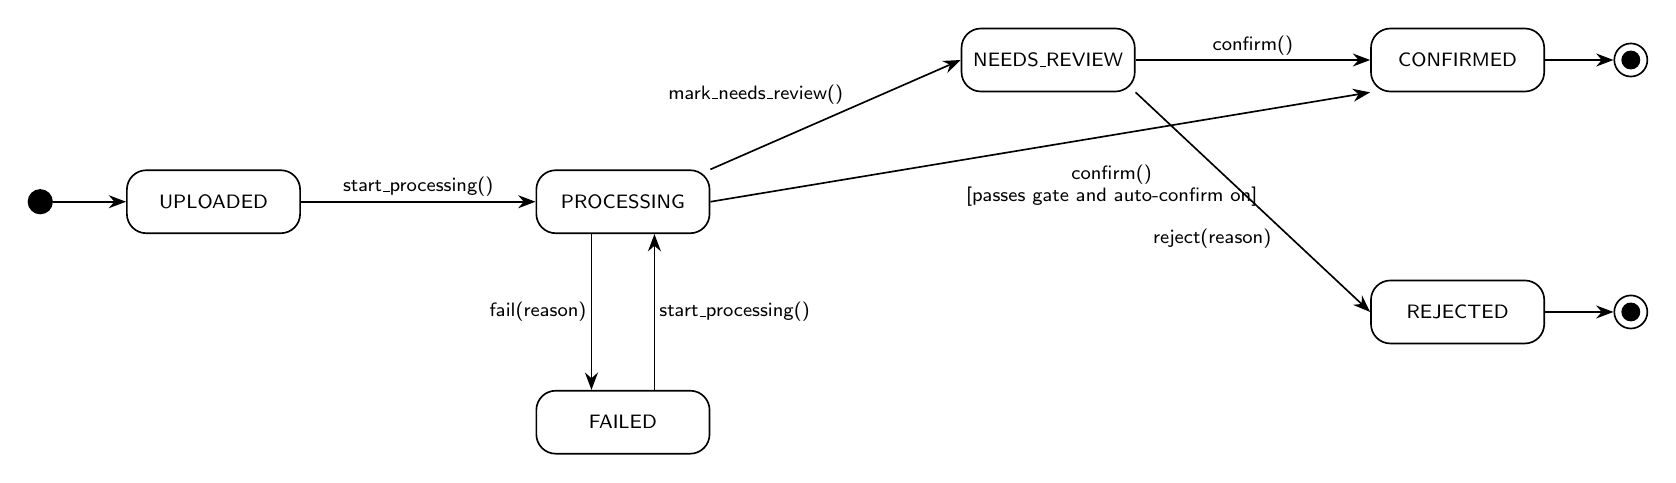
\begin{tikzpicture}
  \node[initial] (i) at (0,0) {};
  \node[state] (up) at (2.2,0) {UPLOADED};
  \node[state] (pr) at (7.4,0) {PROCESSING};
  \node[state] (nr) at (12.8,1.8) {NEEDS\_REVIEW};
  \node[state] (fa) at (7.4,-2.8) {FAILED};
  \node[state] (co) at (18.0,1.8) {CONFIRMED};
  \node[state] (re) at (18.0,-1.4) {REJECTED};
  \node[final] (f1) at (20.2,1.8) {};
  \node[final] (f2) at (20.2,-1.4) {};
  \draw[tr] (i) -- (up);
  \draw[tr] (up) -- node[slbl, above] {start\_processing()} (pr);
  \draw[tr] (pr.north east) -- node[slbl, above left, pos=0.55] {mark\_needs\_review()} (nr.west);
  \draw[tr] (pr.east) -- node[slbl, below right, pos=0.38] {confirm()\\ {[passes gate and auto-confirm on]}} (co.south west);
  \draw[tr] ([xshift=-4mm]pr.south) -- node[slbl, left] {fail(reason)} ([xshift=-4mm]fa.north);
  \draw[tr] ([xshift=4mm]fa.north) -- node[slbl, right] {start\_processing()} ([xshift=4mm]pr.south);
  \draw[tr] (nr) -- node[slbl, above] {confirm()} (co);
  \draw[tr] (nr.south east) -- node[slbl, below left, pos=0.6] {reject(reason)} (re.west);
  \draw[tr] (co) -- (f1);
  \draw[tr] (re) -- (f2);
\end{tikzpicture}}

\newcommand{\notificationstate}{%
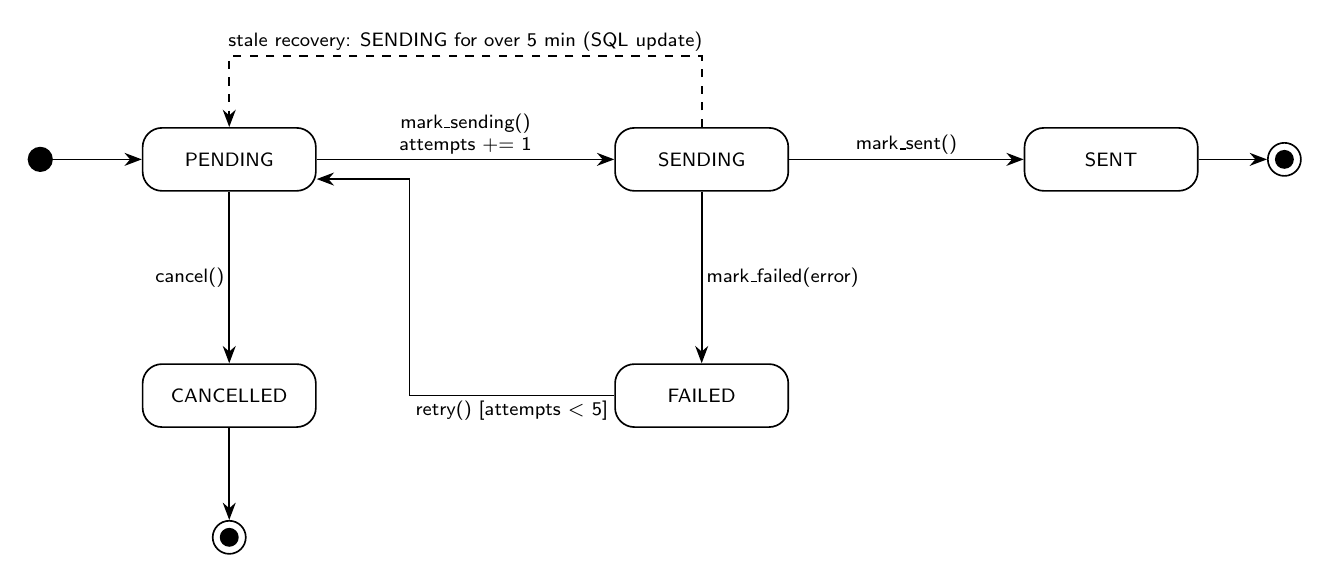
\begin{tikzpicture}
  \node[initial] (i) at (0,0) {};
  \node[state] (pe) at (2.4,0) {PENDING};
  \node[state] (se) at (8.4,0) {SENDING};
  \node[state] (sent) at (13.6,0) {SENT};
  \node[state] (fa) at (8.4,-3.0) {FAILED};
  \node[state] (ca) at (2.4,-3.0) {CANCELLED};
  \node[final] (f1) at (15.8,0) {};
  \node[final] (f2) at (2.4,-4.8) {};
  \draw[tr] (i) -- (pe);
  \draw[tr] (pe) -- node[slbl, above] {mark\_sending()\\attempts += 1} (se);
  \draw[tr] (se) -- node[slbl, above] {mark\_sent()} (sent);
  \draw[tr, dashed] (se.north) -- ++(0,0.9) -| node[slbl, pos=0.25, above] {stale recovery: SENDING for over 5 min (SQL update)} (pe.north);
  \draw[tr] (se) -- node[slbl, right] {mark\_failed(error)} (fa);
  \draw[tr] (fa.west) -- node[slbl, below] {retry() [attempts $<$ 5]} ++(-2.6,0) |- ([yshift=-2.5mm]pe.east);
  \draw[tr] (pe) -- node[slbl, left] {cancel()} (ca);
  \draw[tr] (sent) -- (f1);
  \draw[tr] (ca) -- (f2);
\end{tikzpicture}}

\newcommand{\uploadstate}{%
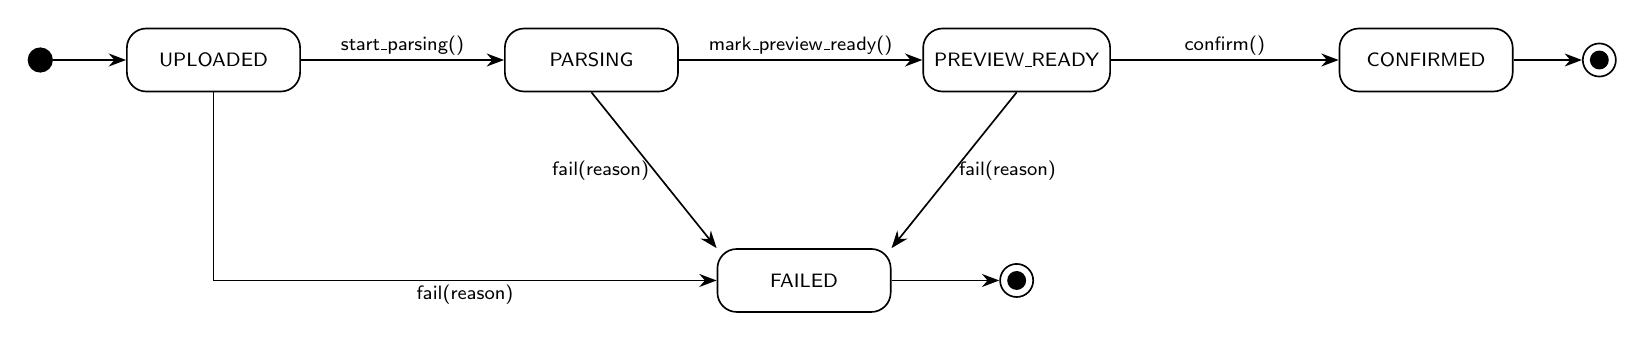
\begin{tikzpicture}
  \node[initial] (i) at (0,0) {};
  \node[state] (up) at (2.2,0) {UPLOADED};
  \node[state] (pa) at (7.0,0) {PARSING};
  \node[state] (pv) at (12.4,0) {PREVIEW\_READY};
  \node[state] (co) at (17.6,0) {CONFIRMED};
  \node[state] (fa) at (9.7,-2.8) {FAILED};
  \node[final] (f1) at (19.8,0) {};
  \node[final] (f2) at (12.4,-2.8) {};
  \draw[tr] (i) -- (up);
  \draw[tr] (up) -- node[slbl, above] {start\_parsing()} (pa);
  \draw[tr] (pa) -- node[slbl, above] {mark\_preview\_ready()} (pv);
  \draw[tr] (pv) -- node[slbl, above] {confirm()} (co);
  \draw[tr] (up.south) |- node[slbl, pos=0.75, below] {fail(reason)} (fa.west);
  \draw[tr] (pa.south) -- node[slbl, left, pos=0.5] {fail(reason)} (fa.north west);
  \draw[tr] (pv.south) -- node[slbl, right, pos=0.5] {fail(reason)} (fa.north east);
  \draw[tr] (fa) -- (f2);
  \draw[tr] (co) -- (f1);
\end{tikzpicture}}


\titleformat{\section}{\fontsize{16}{20}\selectfont\bfseries}{\thesection.}{0.5em}{}
\titleformat{\subsection}{\fontsize{14}{17}\selectfont\bfseries}{\thesubsection}{0.6em}{}
\titlespacing*{\section}{0pt}{0pt}{14pt}
\titlespacing*{\subsection}{0pt}{14pt}{8pt}
\newcommand{\theory}[1]{\par\medskip\needspace{4\baselineskip}\noindent\textbf{\textit{#1}}\par\smallskip}
\newcommand{\head}[1]{\par\medskip\needspace{4\baselineskip}\noindent\textbf{#1}\par\smallskip}
\setlength{\parskip}{6pt}
\setlength{\emergencystretch}{2.5em}
\setlength{\parindent}{0pt}
\linespread{1.12}
\captionsetup{labelsep=colon, font=normalsize}
\renewcommand{\arraystretch}{1.3}
\newcolumntype{Y}{>{\RaggedRight\arraybackslash}X}
\setlist{itemsep=2pt, topsep=4pt}

\renewcommand{\cftsecfont}{\bfseries}
\renewcommand{\cftsecpagefont}{\bfseries}
\renewcommand{\cftsecleader}{\hfill}
\renewcommand{\cftsubsecleader}{\cftdotfill{\cftdotsep}}
\setlength{\cftbeforesecskip}{10pt}
\setlength{\cftbeforesubsecskip}{4pt}
\renewcommand{\cfttoctitlefont}{\fontsize{16}{20}\selectfont\bfseries}
\renewcommand{\cftloftitlefont}{\fontsize{16}{20}\selectfont\bfseries}
\renewcommand{\cftlottitlefont}{\fontsize{16}{20}\selectfont\bfseries}
\renewcommand{\contentsname}{Table of Contents}
\renewcommand{\listfigurename}{List of Figures}
\renewcommand{\listtablename}{List of Tables}
\setcounter{tocdepth}{2}

\newcommand{\newsection}[2]{\clearpage\section{#1}\label{#2}}

\begin{document}
\justifying
\sloppy

\pagenumbering{arabic}
\begin{titlepage}
  \centering
  \vspace*{0.6cm}
  
\includegraphics[width=5.2cm]{figures/ramaiah-logo.png}\par
  \vspace{1.0cm}
  {\large\bfseries RAMAIAH INSTITUTE OF TECHNOLOGY, BANGALORE -- 560054\par}
  {\large\bfseries (Autonomous Institute, Affiliated to VTU)\par}
  {\large\bfseries Department of Computer Science \& Engineering\par}
  \vspace{0.2cm}
  {\Large\bfseries Practical Assignment Report\par}
  \vspace{1.1cm}
  {\fontsize{19}{24}\selectfont\bfseries FacultyDesk: A Scheduling, Reminder and\\[2pt] Task Management System for College Faculty\par}
  \vspace{0.9cm}
  {\fontsize{19}{24}\selectfont\itshape\bfseries CSE556: Object-Oriented Analysis and Design\par}
  \vspace{1.0cm}
  {\large\bfseries SUBMITTED BY:\par}
  \vspace{0.3cm}
  {\renewcommand{\arraystretch}{1.35}
  \begin{tabular}{|l|c|c|}
  \hline
  \textbf{Name} & \textbf{USN} & \textbf{Sec} \\ \hline
  Krish Kumar Sharma & 1MS25CS408 & 5 `C' \\ \hline
  Thanishq Vijaykumar & 1MS24CS202 & 5 `D' \\ \hline
  Santhosha Naik D K & 1MS25CS416 & 5 `D' \\ \hline
  \end{tabular}\par}
  \vspace{0.9cm}
  {\small\sffamily\bfseries SUPERVISED BY:\par}
  \vspace{0.15cm}
  {\bfseries Faculty\par}
  \vspace{0.1cm}
  {\bfseries DR. PARKAVI A\par}
  {\small PROFESSOR\par}
  {\small DEPARTMENT OF CSE\par}
  \vfill
  {\bfseries Sep -- Nov, 2026\par}
  \vspace{0.6cm}
\end{titlepage}
\setcounter{page}{2}

\begin{center}
  
\includegraphics[width=4.2cm]{figures/ramaiah-logo.png}\par
  \vspace{0.6cm}
  {\large\bfseries Department of Computer Science and Engineering\par}
  \vspace{0.15cm}
  {\large\bfseries M S Ramaiah Institute of Technology\par}
  {(Autonomous Institute, Affiliated to VTU)\par}
  {Bangalore -- 54\par}
  \vspace{1.2cm}
  {\fontsize{20}{24}\selectfont\bfseries CERTIFICATE\par}
\end{center}
\vspace{0.8cm}
{\linespread{1.6}\selectfont
This is to certify that \textbf{Krish Kumar Sharma (1MS25CS408)}, \textbf{Thanishq Vijaykumar (1MS24CS202)} and \textbf{Santhosha Naik D K (1MS25CS416)} have completed the ``\textbf{\projecttitle}'' as part of the Practical Assignment for the course \textbf{Object-Oriented Analysis and Design (CSE556)}. We declare that the entire content embodied in this B.E.\ CSE, 5th semester report is not copied.\par}

\vspace{1.6cm}
\noindent
\begin{tabular*}{\textwidth}{@{}l@{\extracolsep{\fill}}r@{}}
\textbf{Submitted by} & \textbf{Guided by} \\[1.2cm]
\rule{4.5cm}{0.4pt} & \rule{4.5cm}{0.4pt} \\
Krish Kumar Sharma (1MS25CS408) & Dr. Parkavi A \\[1.0cm]
\rule{4.5cm}{0.4pt} & Professor, Dept. of CSE \\
Thanishq Vijaykumar (1MS24CS202) & \\[1.0cm]
\rule{4.5cm}{0.4pt} & \\
Santhosha Naik D K (1MS25CS416) & \\
\end{tabular*}
\clearpage

\begin{center}
  
\includegraphics[width=4.2cm]{figures/ramaiah-logo.png}\par
  \vspace{0.6cm}
  {\large\bfseries Department of Computer Science and Engineering\par}
  \vspace{0.15cm}
  {\large\bfseries M S Ramaiah Institute of Technology\par}
  {(Autonomous Institute, Affiliated to VTU)\par}
  {Bangalore -- 54\par}
  \vspace{2cm}
  {\fontsize{20}{24}\selectfont\bfseries Evaluation Sheet\par}
\end{center}
\vspace{1.2cm}
{\renewcommand{\arraystretch}{2.6}
\noindent
\small\begin{tabularx}{\textwidth}{|>{\centering\arraybackslash}p{2.3cm}|Y|>{\centering\arraybackslash}p{3.3cm}|>{\centering\arraybackslash}p{2.7cm}|>{\centering\arraybackslash}p{1.7cm}|}
\hline
\textbf{USN} & \textbf{Name} & \makecell{\textbf{OOAD approach \&}\\\textbf{Explanation Skills}\\\textbf{(5)}} & \makecell{\textbf{Coding \&}\\\textbf{Documentation}\\\textbf{(5)}} & \makecell{\textbf{Total}\\\textbf{Marks}\\\textbf{(10)}} \\ \hline
1MS25CS408 & Krish Kumar Sharma & & & \\ \hline
1MS24CS202 & Thanishq Vijaykumar & & & \\ \hline
1MS25CS416 & Santhosha Naik D K & & & \\ \hline
\end{tabularx}}

\vspace{2cm}
\noindent\textbf{Evaluated By}\\[0.5cm]
{\renewcommand{\arraystretch}{1.6}
\begin{tabular}{@{}ll@{}}
Name: & Dr. Parkavi A \\
Designation: & Professor \\
Department: & Computer Science \& Engineering (AIML) \& CSE (CS), RIT \\
Signature: & \\
\end{tabular}}
\clearpage

\tableofcontents
\clearpage
\listoffigures
\clearpage
\listoftables


\newsection{Abstract}{sec:abstract}

Faculty members in an engineering department follow three separate sources of information: the department timetable for classes, paper circulars for meetings, and verbal or e-mail instructions for documentation work such as CO--PO mapping, internal assessment (IA) marks upload and lab manual updates. None of these sources reminds anyone, clashes between duties are found only when they happen, and the Head of the Department (HOD) has no single view of pending documentation.

\textbf{FacultyDesk} is a web application that brings all three sources into one personal calendar for every faculty member. The HOD uploads the timetable file the department already produces (Excel, CSV or PDF); the system reads every cell, matches teacher initials such as \texttt{CN (KKS)} to faculty accounts and generates each person's weekly classes for the term, skipping holidays. Any faculty member can photograph a meeting circular; optical character recognition (OCR) extracts the date, time, venue and the faculty named in it, and uncertain results go to a review queue where the HOD confirms them. Confirmed meetings appear on every attendee's calendar with clash detection. Reminders are sent by e-mail and web push at times each user chooses, respect quiet hours, and are sent at most once per reminder. A task tracker ranks documentation work by a priority score, alerts before each deadline and escalates overdue work to the HOD.

The system was designed using Object-Oriented Analysis and Design (OOAD). Twenty domain classes carry the business rules; three of them (\texttt{Circular}, \texttt{ScheduledNotification} and \texttt{TimetableUpload}) are explicit state machines. The code follows a four-layer architecture (domain, application, infrastructure, API) and applies the Repository, Unit of Work, Strategy, Factory, Composite and State design patterns. This report presents the business case, the object-oriented analysis, eleven kinds of UML and related diagrams with explanations and use case scenarios, the core algorithms in pseudo code, and the results.

On 13 November 2026, all 83 automated backend tests and all 4 browser end-to-end tests passed on the running system. The sweep-line clash detector gave exactly the same results as a brute-force check on up to 4{,}000 events and was 121 times faster at that size.

\vspace{0.5cm}
\noindent\textbf{Keywords:} Object-oriented analysis and design, UML, use case, class diagram, design patterns, clean architecture, OCR, scheduling, reminders, academic administration.

\newsection{Introduction}{sec:intro}

\subsection{Background}
A typical working week of a faculty member combines three kinds of commitments. \textbf{Classes} come from the department timetable, a spreadsheet grid in which each cell holds a course code, a section and the teacher's initials, for example \texttt{CN (KKS)}. \textbf{Meetings} are announced through paper circulars that are signed, scanned and pinned on the notice board or forwarded as a photo in a group chat. \textbf{Documentation work}, such as CO--PO (course outcome to programme outcome) mapping, IA marks upload, attendance shortage reports and lab manual updates, arrives as instructions with a deadline.

\subsection{Existing System and its Limitations}
In the current manual process each faculty member keeps track of these items personally.
\begin{itemize}
  \item \textbf{No single view.} Classes, meetings and deadlines live in three different places.
  \item \textbf{No reminders.} The timetable, the notice board and the e-mail do not remind anyone.
  \item \textbf{Clashes are found late.} A meeting called during a scheduled class is noticed only on the day.
  \item \textbf{Revisions are missed.} When the timetable changes, every teacher has to read the new sheet again.
  \item \textbf{No follow-up for documentation.} The HOD has to ask each person whether a task is done.
  \item \textbf{Retyping.} General calendar apps require every class and meeting to be entered by hand.
\end{itemize}

\subsection{Proposed System}
FacultyDesk reads the documents the department already produces instead of asking anyone to retype them.
\begin{enumerate}
  \item The HOD uploads the timetable file. The system parses it, matches initials to faculty accounts, shows a preview, and after confirmation generates every class of the term for every teacher.
  \item Anyone uploads a photo or scan of a circular. OCR reads it and proposes a meeting with date, time, venue and attendees. The HOD reviews uncertain results and confirms.
  \item Every faculty member sees classes, meetings and deadlines on one calendar with clash warnings, and can subscribe to it from Google Calendar or Apple Calendar through an iCalendar (ICS) feed [8].
  \item Reminders arrive on the phone (web push) and by e-mail at chosen lead times, outside the user's quiet hours.
  \item Documentation tasks are tracked with deadlines, a priority score, alerts and escalation to the HOD.
\end{enumerate}

\subsection{Technology Used}
\needspace{7\baselineskip}
\begin{xltabular}{\textwidth}{|p{4.2cm}|Y|}
\caption{Technology stack}\\
\hline
\textbf{Layer} & \textbf{Technology} \\ \hline
Backend & Python 3.12, FastAPI, Pydantic v2, SQLAlchemy 2 (async), Alembic migrations \\ \hline
Background jobs & Celery 5 with Redis 7 (worker and Celery Beat scheduler) \\ \hline
Database and files & PostgreSQL 16; MinIO (S3-compatible object storage) \\ \hline
OCR and parsing & Tesseract OCR [6], OpenCV, pdfplumber, openpyxl, rapidfuzz \\ \hline
Notifications & SMTP e-mail (aiosmtplib), Web Push with VAPID keys (pywebpush) \\ \hline
Frontend & Next.js (App Router), TypeScript, Tailwind CSS, FullCalendar, installable PWA \\ \hline
Security & Argon2id password hashing, JWT access tokens, rotating refresh cookies \\ \hline
Quality & ruff, mypy (strict), pytest, Playwright end-to-end tests \\ \hline
Deployment & Docker Compose, Caddy reverse proxy with HTTPS \\ \hline
\end{xltabular}

\subsection{Organisation of the Report}
Section~\ref{sec:objectives} states the problem, objectives and requirements. Section~\ref{sec:overview} explains the object-oriented basics used, the eight modules of the project and the business aspects. Section~\ref{sec:uml} presents the UML models, each with theory, diagram, explanation and tables. Section~\ref{sec:ooad} covers the object-oriented analysis, design and architecture. Section~\ref{sec:impl} gives the core algorithms in pseudo code. Sections~\ref{sec:results} and \ref{sec:discussion} present and discuss the results, and Section~\ref{sec:conclusion} concludes. Section~\ref{sec:literature} lists the 2026 papers surveyed, with proof.

\newsection{Objectives \& Problem Statement}{sec:objectives}

\subsection{Problem Statement}
A college department wants a system that turns its existing timetable files and paper meeting circulars into a personal, clash-aware calendar for every faculty member. The HOD uploads the department timetable; the system must identify each teacher from the initials written in the timetable cells and create that teacher's classes for the whole term, leaving out holidays. Any faculty member may upload a photo of a meeting circular; the system must read the date, time, venue and the names or initials of the invited faculty, and must not place a meeting on anyone's calendar until it is sure of the details or the HOD has confirmed them. Every faculty member must be reminded before each class, meeting and deadline by e-mail or phone notification, at times they choose, but not during their quiet hours, and never twice for the same reminder. The HOD must be able to assign documentation tasks to one teacher, a group or the whole department, see who has completed them, and be alerted when work is overdue.

\subsection{Objectives}
\begin{enumerate}
  \item \textbf{Timetable ingestion:} read Excel, CSV and text-layer PDF timetables, expand merged period cells, resolve initials to faculty accounts, and generate the term's weekly classes while skipping declared holidays.
  \item \textbf{Circular scanning:} accept photos, scans and PDFs of circulars, extract date, time, venue, agenda and attendees with OCR, and send uncertain extractions to an HOD review queue.
  \item \textbf{Personal calendar:} show classes, meetings and deadlines in one view, detect overlapping events, find common free slots for a group, and publish a private ICS feed.
  \item \textbf{Reminders:} deliver reminders by e-mail and web push at user-chosen lead times, honour quiet hours, retry failed sends and never send the same reminder twice.
  \item \textbf{Documentation tasks:} create and assign tasks, rank them by a transparent priority score, alert before the deadline and escalate overdue work.
  \item \textbf{Object-oriented design:} model the domain with classes that hold their own rules, keep business logic independent of frameworks, and document the design in UML.
\end{enumerate}

\subsection{Functional Requirements}
\begin{xltabular}{\textwidth}{|p{1.4cm}|Y|p{2.6cm}|}
\caption{Functional requirements}\\
\hline
\textbf{ID} & \textbf{Requirement} & \textbf{Actor} \\ \hline
FR-01 & Log in with e-mail and password; access depends on role (Admin, HOD, Faculty). & All \\ \hline
FR-02 & Manage departments, faculty accounts (with initials and aliases), terms and holidays; bulk import from CSV/XLSX. & Admin, HOD \\ \hline
FR-03 & Upload a timetable, preview parsed slots and unresolved initials, and confirm. & HOD, Admin \\ \hline
FR-04 & Generate weekly class events for the term, skipping holidays. & System \\ \hline
FR-05 & Upload a circular photo, scan or PDF and extract meeting details by OCR. & Faculty, HOD \\ \hline
FR-06 & Review, correct, confirm or reject extracted circulars. & HOD \\ \hline
FR-07 & View the personal calendar; create, move and cancel events with clash warnings. & Faculty, HOD \\ \hline
FR-08 & Find common free slots for a group of faculty. & HOD \\ \hline
FR-09 & Subscribe to a private ICS calendar feed and rotate its secret token. & Faculty \\ \hline
FR-10 & Set reminder lead times, channels and quiet hours; register for web push. & Faculty \\ \hline
FR-11 & Send due reminders exactly once by e-mail and web push. & Scheduler \\ \hline
FR-12 & Create personal tasks; assign tasks to a person, a group or the department from templates. & Faculty, HOD \\ \hline
FR-13 & Rank tasks by priority, alert before deadlines, send daily overdue alerts and HOD escalations. & System \\ \hline
FR-14 & Show the HOD a dashboard of completion rate and overdue tasks per faculty member. & HOD \\ \hline
\end{xltabular}

\subsection{Non-Functional Requirements}
\needspace{7\baselineskip}
\begin{xltabular}{\textwidth}{|p{3.2cm}|Y|}
\caption{Non-functional requirements}\\
\hline
\textbf{Quality} & \textbf{Requirement and how it is met} \\ \hline
Correctness & All times stored in UTC and shown in India Standard Time; business rules covered by automated tests. \\ \hline
Reliability & Reminders survive worker crashes (stale-send recovery) and are never duplicated (unique idempotency key). \\ \hline
Security & Argon2id password hashing, 15-minute access tokens, rotating refresh tokens with reuse detection, role checks, rate-limited log-in. \\ \hline
Safety of uploads & File type checked from its first bytes, 15 MB size limit, image pixel limit, PDF page limit. \\ \hline
Usability & Mobile-first web app that installs on a phone; works with existing calendar apps through ICS. \\ \hline
Maintainability & Four-layer architecture, one class per use case, strict type checking. \\ \hline
Deployability & Runs on one department server with Docker Compose; no paid service needed. \\ \hline
\end{xltabular}

\subsection{Scope and Constraints}
\begin{itemize}
  \item Three human roles: Admin, HOD and Faculty. A background scheduler acts as a fourth, non-human actor.
  \item Scanned timetable PDFs without a text layer are rejected with guidance; scanned circulars are read with OCR.
  \item The system does not create timetables; it reads timetables that the department has already prepared.
\end{itemize}

\newsection{Object Basics and Project Overview}{sec:overview}

\subsection{Object Basics}
Object-oriented analysis and design views a system as a set of objects that work together. Each object holds data and the operations that act on that data. The table below defines each basic concept and shows where it appears in FacultyDesk.

{\small
\needspace{7\baselineskip}
\begin{xltabular}{\textwidth}{|p{2.6cm}|Y|Y|}
\caption{Object basics with project examples}\\
\hline
\textbf{Concept} & \textbf{Meaning} & \textbf{Example in FacultyDesk} \\ \hline
Object & A thing with identity, state and behaviour. & One uploaded meeting circular, with its text, extracted fields and status. \\ \hline
Class & A template that defines the attributes and operations of similar objects. & \texttt{Circular} defines \texttt{ocr\_text}, \texttt{confidence}, \texttt{status} and \texttt{confirm()}, \texttt{reject()}. \\ \hline
Encapsulation & Data is changed only through the object's own operations. & A \texttt{ScheduledNotification} changes status only through \texttt{mark\_sending()}, \texttt{mark\_sent()}, \texttt{mark\_failed()}, \texttt{retry()} and \texttt{cancel()}; any illegal change raises an error. \\ \hline
Abstraction & Showing what an object does and hiding how. & \texttt{UnitOfWork} and the repository interfaces describe what storage must do, not how the database does it. \\ \hline
Inheritance & A class reuses and specialises another class. & \texttt{XlsxTimetableParser}, \texttt{CsvTimetableParser} and \texttt{PdfTimetableParser} inherit from \texttt{TimetableParser}. \\ \hline
Polymorphism & The same call behaves differently depending on the object. & \texttt{parser.parse(content)} reads Excel, CSV or PDF; \texttt{notifier.send(...)} sends an e-mail or a push message. \\ \hline
Value object & An immutable object defined only by its value. & \texttt{Initials} (2 to 5 capital letters), \texttt{TimeSlot}, \texttt{QuietHours}. \\ \hline
Association & A structural link between classes. & A \texttt{FacultyProfile} belongs to a \texttt{Department}. \\ \hline
Composition & A whole that owns its parts; parts cannot exist alone. & An \texttt{Event} owns its \texttt{EventAttendee} objects; an \texttt{AcademicTerm} owns its \texttt{Holiday} objects. \\ \hline
\end{xltabular}}

\subsection{System Overview}
Figure~\ref{fig:arch} shows the overall structure. Users work in a web application in the browser or on the phone. Requests reach the FastAPI server through a Caddy reverse proxy. Slow work (reading timetables, OCR, sending reminders) runs in Celery workers, and Celery Beat starts periodic jobs. Data lives in PostgreSQL; uploaded files and backups live in MinIO.

\begin{figure}[!htbp]
\centering
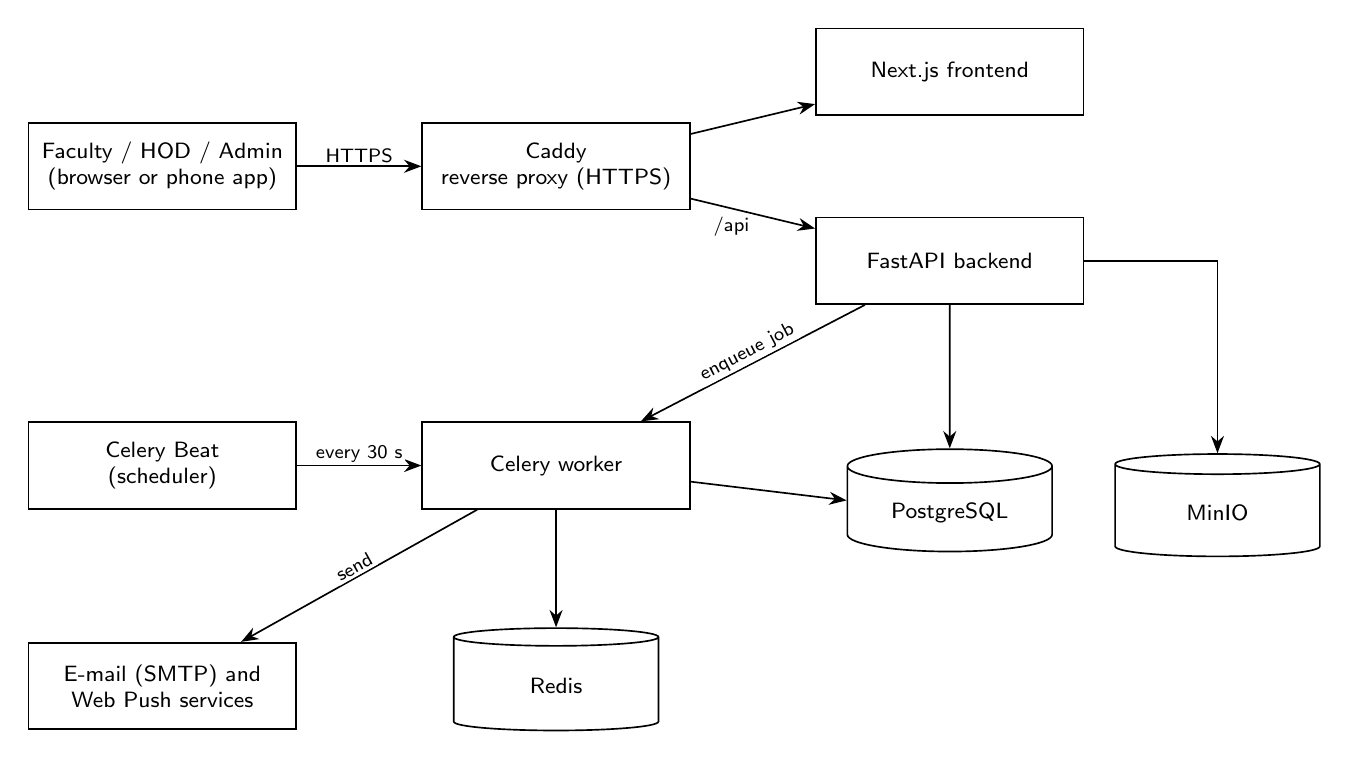
\begin{tikzpicture}[
  box/.style={rectangle, draw, semithick, align=center, font=\footnotesize, minimum width=3.4cm, minimum height=1.1cm},
  db/.style={cylinder, shape border rotate=90, aspect=0.25, draw, semithick, align=center, font=\footnotesize, minimum width=2.6cm, minimum height=1.3cm},
  ar/.style={semithick, -{Stealth[length=2.2mm]}},
  l/.style={font=\scriptsize, fill=white, inner sep=1pt}]
  \node[box] (user) at (0,0) {Faculty / HOD / Admin\\(browser or phone app)};
  \node[box] (caddy) at (5,0) {Caddy\\reverse proxy (HTTPS)};
  \node[box] (fe) at (10,1.2) {Next.js frontend};
  \node[box] (api) at (10,-1.2) {FastAPI backend};
  \node[box] (worker) at (5,-3.8) {Celery worker};
  \node[box] (beat) at (0,-3.8) {Celery Beat\\(scheduler)};
  \node[db] (pg) at (10,-4.4) {PostgreSQL};
  \node[db] (redis) at (5,-6.6) {Redis};
  \node[db] (minio) at (13.4,-4.4) {MinIO};
  \node[box] (mail) at (0,-6.6) {E-mail (SMTP) and\\Web Push services};
  \draw[ar] (user) -- node[l, above] {HTTPS} (caddy);
  \draw[ar] (caddy) -- (fe);
  \draw[ar] (caddy) -- node[l, below left] {/api} (api);
  \draw[ar] (api) -- (pg);
  \draw[ar] (api.east) -| (minio);
  \draw[ar] (api) -- node[l, sloped, above] {enqueue job} (worker);
  \draw[ar] (beat) -- node[l, above] {every 30 s} (worker);
  \draw[ar] (worker) -- (pg);
  \draw[ar] (worker) -- (redis);
  \draw[ar] (worker) -- node[l, sloped, above] {send} (mail);
\end{tikzpicture}
\caption{High-level architecture of FacultyDesk}
\label{fig:arch}
\end{figure}

\subsection{Project Modules}
The system is divided into eight modules. Each module has its own use-case classes, its own set of API endpoints and its own screens, and all modules share one domain model.

\head{Module 1: Identity and Access}
Handles log-in, log-out and password change. Passwords are hashed with Argon2id. A short-lived access token (15 minutes) is kept in memory, and a refresh token (7 days) is kept in an httpOnly cookie and replaced on every use; if an old refresh token is presented again, the whole token family is revoked. One \texttt{AuthorisationPolicy} class decides what each role may do. Log-in attempts are rate-limited per IP address and per account.\par\smallskip
{\RaggedRight\textit{Main classes:} \texttt{LoginUseCase}, \texttt{RefreshTokenUseCase}, \texttt{LogoutUseCase}, \texttt{AuthorisationPolicy}, \texttt{Principal}.\par}

\head{Module 2: Directory and Academic Calendar}
Maintains departments, faculty accounts with their initials and aliases, academic terms and holidays. Faculty can be imported in bulk from CSV or Excel with a row-by-row validation report.\par\smallskip
{\RaggedRight\textit{Main classes:} \texttt{CreateFacultyUseCase}, \texttt{UpdateFacultyUseCase}, \texttt{BulkImportFacultyUseCase}, \texttt{ManageTermsUseCase}.\par}

\head{Module 3: Timetable Ingestion}
Accepts the department timetable, chooses a parser from the file's first bytes, expands merged period cells, splits co-teacher cells such as \texttt{KKS/RNS}, and resolves each initials token in three tiers (exact initials, alias, fuzzy match). The HOD sees a preview and the unresolved tokens before confirming.\par\smallskip
{\RaggedRight\textit{Main classes:} \texttt{UploadTimetableUseCase}, \texttt{ParseTimetableUseCase}, \texttt{ConfirmTimetableUseCase}, \texttt{TimetableParserFactory}, \texttt{InitialsResolver}.\par}

\head{Module 4: Circular Scanning}
Reads meeting circulars. Images are cleaned (grey scale, noise removal, thresholding, deskewing) and read by Tesseract. The extractor finds date, time, venue, title, agenda and attendees, and a review gate decides whether the circular may be confirmed automatically or needs the HOD.\par\smallskip
{\RaggedRight\textit{Main classes:} \texttt{UploadCircularUseCase}, \texttt{ProcessCircularUseCase}, \texttt{ConfirmCircularUseCase}, \texttt{RejectCircularUseCase}, \texttt{OcrEngine}, \texttt{CircularExtractor}.\par}

\head{Module 5: Calendar}
Keeps every class, meeting and deadline as an \texttt{Event} with attendees. It detects clashes with a sweep-line algorithm, finds common free slots, publishes the ICS feed, and every night extends class events 21 days ahead.\par\smallskip
{\RaggedRight\textit{Main classes:} \texttt{CreateEventUseCase}, \texttt{UpdateEventUseCase}, \texttt{SweepLineClashDetector}, \texttt{FreeSlotFinder}, \texttt{GenerateIcsFeedUseCase}, \texttt{MaterialiseTimetableEventsUseCase}.\par}

\head{Module 6: Reminders and Notifications}
Plans one \texttt{ScheduledNotification} per attendee, lead time and channel, shifts reminders out of quiet hours, and sends due reminders every 30 seconds by e-mail and web push.\par\smallskip
{\RaggedRight\textit{Main classes:} \texttt{ReminderPlanner}, \texttt{ReminderDispatcher}, \texttt{CompositeNotifier}, \texttt{EmailNotifier}, \texttt{WebPushNotifier}.\par}

\head{Module 7: Tasks and Escalation}
Manages personal and assigned documentation tasks with templates (CO--PO mapping, IA marks upload, attendance shortage report, lab manual update, course file submission). Tasks are ranked by a priority score; alerts go out 72 hours, 24 hours and 2 hours before the deadline and daily after it, and overdue work is escalated to the HOD.\par\smallskip
{\RaggedRight\textit{Main classes:} \texttt{CreateTaskUseCase}, \texttt{AssignTaskUseCase}, \texttt{CompleteTaskUseCase}, \texttt{ReopenTaskUseCase}, \texttt{GetHodDashboardUseCase}.\par}

\head{Module 8: Operations}
Checks every upload for type, size and decompression attacks, backs up the database every night to object storage with 14-day retention, and reports reminder delivery metrics to the Admin.\par\smallskip
{\RaggedRight\textit{Main classes:} \texttt{BackupService}, upload guard, metrics endpoints.\par}

\subsection{Business Aspects}

\head{Stakeholders and Benefits}
\needspace{7\baselineskip}
{\small\begin{xltabular}{\textwidth}{|p{3.2cm}|Y|Y|}
\caption{Stakeholders and benefits}\\
\hline
\textbf{Stakeholder} & \textbf{Need} & \textbf{Benefit from FacultyDesk} \\ \hline
Faculty member & Know every class, meeting and deadline on time. & One calendar, reminders on phone and e-mail, clash warnings. \\ \hline
HOD & Distribute the timetable and meetings; track documentation. & Upload once for everyone; dashboard of completion and overdue work. \\ \hline
Department office & Avoid retyping schedules and chasing people. & Works directly from the existing timetable file and circular. \\ \hline
College management & Accreditation work (NBA, NAAC) done on time. & Record of assigned and completed documentation tasks. \\ \hline
\end{xltabular}}

\head{Business Process: Before and After}
\needspace{7\baselineskip}
{\small\begin{xltabular}{\textwidth}{|p{3.0cm}|Y|Y|}
\caption{Business process comparison}\\
\hline
\textbf{Activity} & \textbf{Before (manual)} & \textbf{With FacultyDesk} \\ \hline
Timetable revision & New sheet circulated; each teacher re-reads it. & HOD uploads the file once; everyone's classes regenerate. \\ \hline
Meeting circular & Paper notice or chat photo. & Photo uploaded, OCR proposes the meeting, HOD confirms, attendees are reminded. \\ \hline
Documentation deadline & Verbal or e-mail reminder. & Task with priority, alerts at 72 h, 24 h and 2 h, daily overdue alerts, HOD escalation. \\ \hline
Clash between duties & Found on the day. & Shown when the event is created; free-slot finder suggests another time. \\ \hline
\end{xltabular}}

\head{Feasibility}
\begin{itemize}
  \item \textbf{Technical:} built entirely with mature open-source components; runs on one server with Docker Compose.
  \item \textbf{Economic:} no licence cost. Running cost is one server (a department machine or a cloud virtual machine) and an SMTP relay for e-mail; web push uses the browser vendors' free push services. Hardware cost and time saved were not measured; they need a pilot in a department.
  \item \textbf{Operational:} faculty keep using the documents they already produce; the app installs on phones and exports to existing calendar apps.
\end{itemize}

\head{Risks and Controls}
\needspace{7\baselineskip}
{\small\begin{xltabular}{\textwidth}{|p{4.0cm}|Y|}
\caption{Risks and controls}\\
\hline
\textbf{Risk} & \textbf{Control in the design} \\ \hline
Wrong meeting from a bad OCR read & Review gate: document confidence $\ge 70$, date and time confidence $\ge 0.85$, every attendee resolved, no duplicate; otherwise the HOD reviews. \\ \hline
Class assigned to the wrong teacher & Exact initials first, then alias, then fuzzy match only above similarity 0.85 with a 0.10 margin; ambiguous tokens are reported, never guessed. \\ \hline
Duplicate or lost reminders & Unique idempotency key per (target, user, offset, channel); row locking with \texttt{SKIP LOCKED}; recovery of stuck sends. \\ \hline
Exposure of personal data & Hashed passwords, short-lived tokens, role checks, private ICS links that can be rotated. \\ \hline
Data loss & Nightly compressed database backup with 14-day retention and a tested restore. \\ \hline
\end{xltabular}}

\newcommand{\symactor}{\tikz[baseline=-0.1cm, scale=0.55, every node/.style={font=\tiny}]{\pic{actor={}};}}
\newcommand{\symuc}{\tikz[baseline=-0.1cm]\node[ellipse, draw, font=\scriptsize, inner sep=1.5pt]{Use Case};}
\newcommand{\symsys}{\tikz[baseline=-0.1cm]{\draw (0,0.3) rectangle (2,-0.3); \node[font=\tiny] at (1,0.15) {System};}}
\newcommand{\symline}{\tikz[baseline=-0.1cm]\draw (0,0) -- (2,0);}
\newcommand{\symarrow}[1]{\tikz[baseline=-0.1cm]{\draw[dashed, -{Stealth[length=1.6mm]}] (0,0) -- (2,0); \node[font=\tiny, above] at (1,0) {#1};}}
\newcommand{\symgen}{\tikz[baseline=-0.1cm]\draw[-{Triangle[open, length=2.2mm, width=2.2mm]}] (0,0) -- (2,0);}
\newcommand{\symreal}{\tikz[baseline=-0.1cm]\draw[dashed, -{Triangle[open, length=2.2mm, width=2.2mm]}] (0,0) -- (2,0);}
\newcommand{\symdep}{\tikz[baseline=-0.1cm]\draw[dashed, -{Stealth[length=1.6mm]}] (0,0) -- (2,0);}
\newcommand{\symagg}{\tikz[baseline=-0.1cm]\draw[{Diamond[open, length=2.6mm, width=1.8mm]}-] (0,0) -- (2,0);}
\newcommand{\symcomp}{\tikz[baseline=-0.1cm]\draw[{Diamond[length=2.6mm, width=1.8mm]}-] (0,0) -- (2,0);}
\newcommand{\symsync}{\tikz[baseline=-0.1cm]\draw[-{Triangle[length=2mm, width=2mm]}] (0,0) -- (2,0);}
\newcommand{\symasync}{\tikz[baseline=-0.1cm]\draw[-{Stealth[open, length=2mm]}] (0,0) -- (2,0);}
\newcommand{\symreply}{\tikz[baseline=-0.1cm]\draw[dashed, -{Stealth[open, length=2mm]}] (2,0) -- (0,0);}
\newcommand{\symlifeline}{\tikz[baseline=-0.25cm]{\node[draw, font=\tiny, inner sep=2pt] (o) at (0,0) {:Object}; \draw[dashed] (o.south) -- ++(0,-0.4);}}
\newcommand{\syminit}{\tikz[baseline=-0.1cm]\fill (0,0) circle (1.4mm);}
\newcommand{\symfinal}{\tikz[baseline=-0.1cm]{\draw (0,0) circle (1.8mm); \fill (0,0) circle (1.1mm);}}
\newcommand{\symstate}[1]{\tikz[baseline=-0.1cm]\node[draw, rounded corners=4pt, font=\scriptsize, minimum width=1.8cm]{#1};}
\newcommand{\symtrans}{\tikz[baseline=-0.1cm]{\draw[-{Stealth[length=1.6mm]}] (0,0) -- (2,0); \node[font=\tiny, above] at (1,0) {event [guard] / action};}}
\newcommand{\symdecision}{\tikz[baseline=-0.1cm]\node[diamond, draw, minimum size=4mm, inner sep=0pt]{};}
\newcommand{\symfork}{\tikz[baseline=-0.1cm]\fill (0,-0.05) rectangle (2,0.05);}
\newcommand{\symflow}{\tikz[baseline=-0.1cm]\draw[-{Stealth[length=1.6mm]}] (0,0) -- (2,0);}
\newcommand{\sympkg}{\tikz[baseline=-0.1cm]{\draw (0,0.25) rectangle (0.6,0.4); \draw (0,0.25) rectangle (1.6,-0.3); \node[font=\tiny] at (0.8,-0.03) {package};}}
\newcommand{\symcompnt}{\tikz[baseline=-0.1cm]{\node[draw, font=\tiny, align=center, inner sep=2pt] {<{}<component>{}>\\Name};}}
\newcommand{\symball}{\tikz[baseline=-0.1cm]{\draw (0,0) -- (0.9,0); \draw[fill=white] (1.05,0) circle (1.5mm);}}
\newcommand{\symnode}{\tikz[baseline=-0.1cm]{\draw (0,0.25) rectangle (1.4,-0.35); \draw (0,0.25) -- (0.2,0.42) -- (1.6,0.42) -- (1.6,-0.18) -- (1.4,-0.35); \draw (1.4,0.25) -- (1.6,0.42); \node[font=\tiny] at (0.7,-0.05) {Node};}}

\newcommand{\ucscenario}[7]{%
\needspace{7\baselineskip}
\begin{xltabular}{\textwidth}{|p{3.4cm}|Y|}
\caption{Use case scenario: #2}\\
\hline
\textbf{Use Case ID} & #1 \\ \hline
\textbf{Use Case Name} & #2 \\ \hline
\textbf{Actors} & #3 \\ \hline
\textbf{Precondition} & #4 \\ \hline
\textbf{Main Flow} & #5 \\ \hline
\textbf{Alternative Flow} & #6 \\ \hline
\textbf{Postcondition} & #7 \\ \hline
\end{xltabular}}

\newsection{UML Modelling}{sec:uml}

The Unified Modeling Language (UML) is the standard visual language for specifying, constructing and documenting the parts of an object-oriented system [1], [2]. This section models FacultyDesk with the main UML diagrams. For each diagram it gives the theory and notation, the diagram for the project, an explanation, supporting tables and a short conclusion. All class, method, state and attribute names in the diagrams are taken from the project's source code.

\needspace{7\baselineskip}
\begin{xltabular}{\textwidth}{|p{4.6cm}|p{3cm}|Y|}
\caption{UML diagrams presented in this report}\\
\hline
\textbf{Diagram} & \textbf{Kind} & \textbf{What it shows for FacultyDesk} \\ \hline
Use case diagram & Behavioural & Actors and the services the system gives them \\ \hline
Class diagram & Structural & Domain classes, attributes, operations and relations \\ \hline
Sequence diagram & Interaction & Time order of messages in three key flows \\ \hline
Collaboration diagram & Interaction & Objects and numbered messages when a circular is confirmed \\ \hline
Statechart diagram & Behavioural & Life cycles of Circular, ScheduledNotification and TimetableUpload \\ \hline
Activity diagram & Behavioural & Workflow of timetable ingestion across three swimlanes \\ \hline
Package diagram & Structural & Code packages and their dependencies \\ \hline
Component diagram & Structural & Runtime components and the interfaces between them \\ \hline
Deployment diagram & Structural & Containers on the department server and the network links \\ \hline
Entity--relationship diagram & Data model & Database tables, keys and relations \\ \hline
\end{xltabular}

\subsection{Use Case Diagram}

\theory{Theory}
A use case diagram is a behavioural UML diagram that gives a high-level picture of \emph{what} a system offers to its users, without describing \emph{how} each function is built. It contains the system boundary, the actors outside it, the use cases inside it, and the relationships among them.
\begin{itemize}
  \item \textbf{Actor:} an external role that interacts with the system to reach a goal. A \emph{primary actor} starts the use case; a \emph{supporting actor} helps the system deliver it. An actor may be a person or another system, such as a scheduler.
  \item \textbf{Use case:} a unit of functionality that gives an observable result of value to an actor, named with a verb phrase such as ``Upload timetable''.
  \item \textbf{System boundary:} a rectangle that encloses the use cases and defines the scope.
\end{itemize}

\theory{Use Case Notation}
\needspace{7\baselineskip}
\begin{xltabular}{\textwidth}{|p{3cm}|>{\centering\arraybackslash}p{3.3cm}|Y|}
\caption{Use case diagram notation}\\
\hline
\textbf{Element} & \textbf{Symbol} & \textbf{Meaning} \\ \hline
Actor & \symactor & A role played by a user or an external system. \\ \hline
Use case & \symuc & A function the system performs for an actor. \\ \hline
System boundary & \symsys & Encloses the use cases and defines the scope. \\ \hline
Association & \symline & The actor takes part in the use case. \\ \hline
Include & \symarrow{<{}<include>{}>} & The base use case always uses the included one. \\ \hline
Extend & \symarrow{<{}<extend>{}>} & Optional behaviour added to a base use case under a condition. \\ \hline
Generalization & \symgen & The child is a specialised form of the parent. \\ \hline
\end{xltabular}

\begin{figure}[!htbp]
  \centering
  \resizebox{\textwidth}{!}{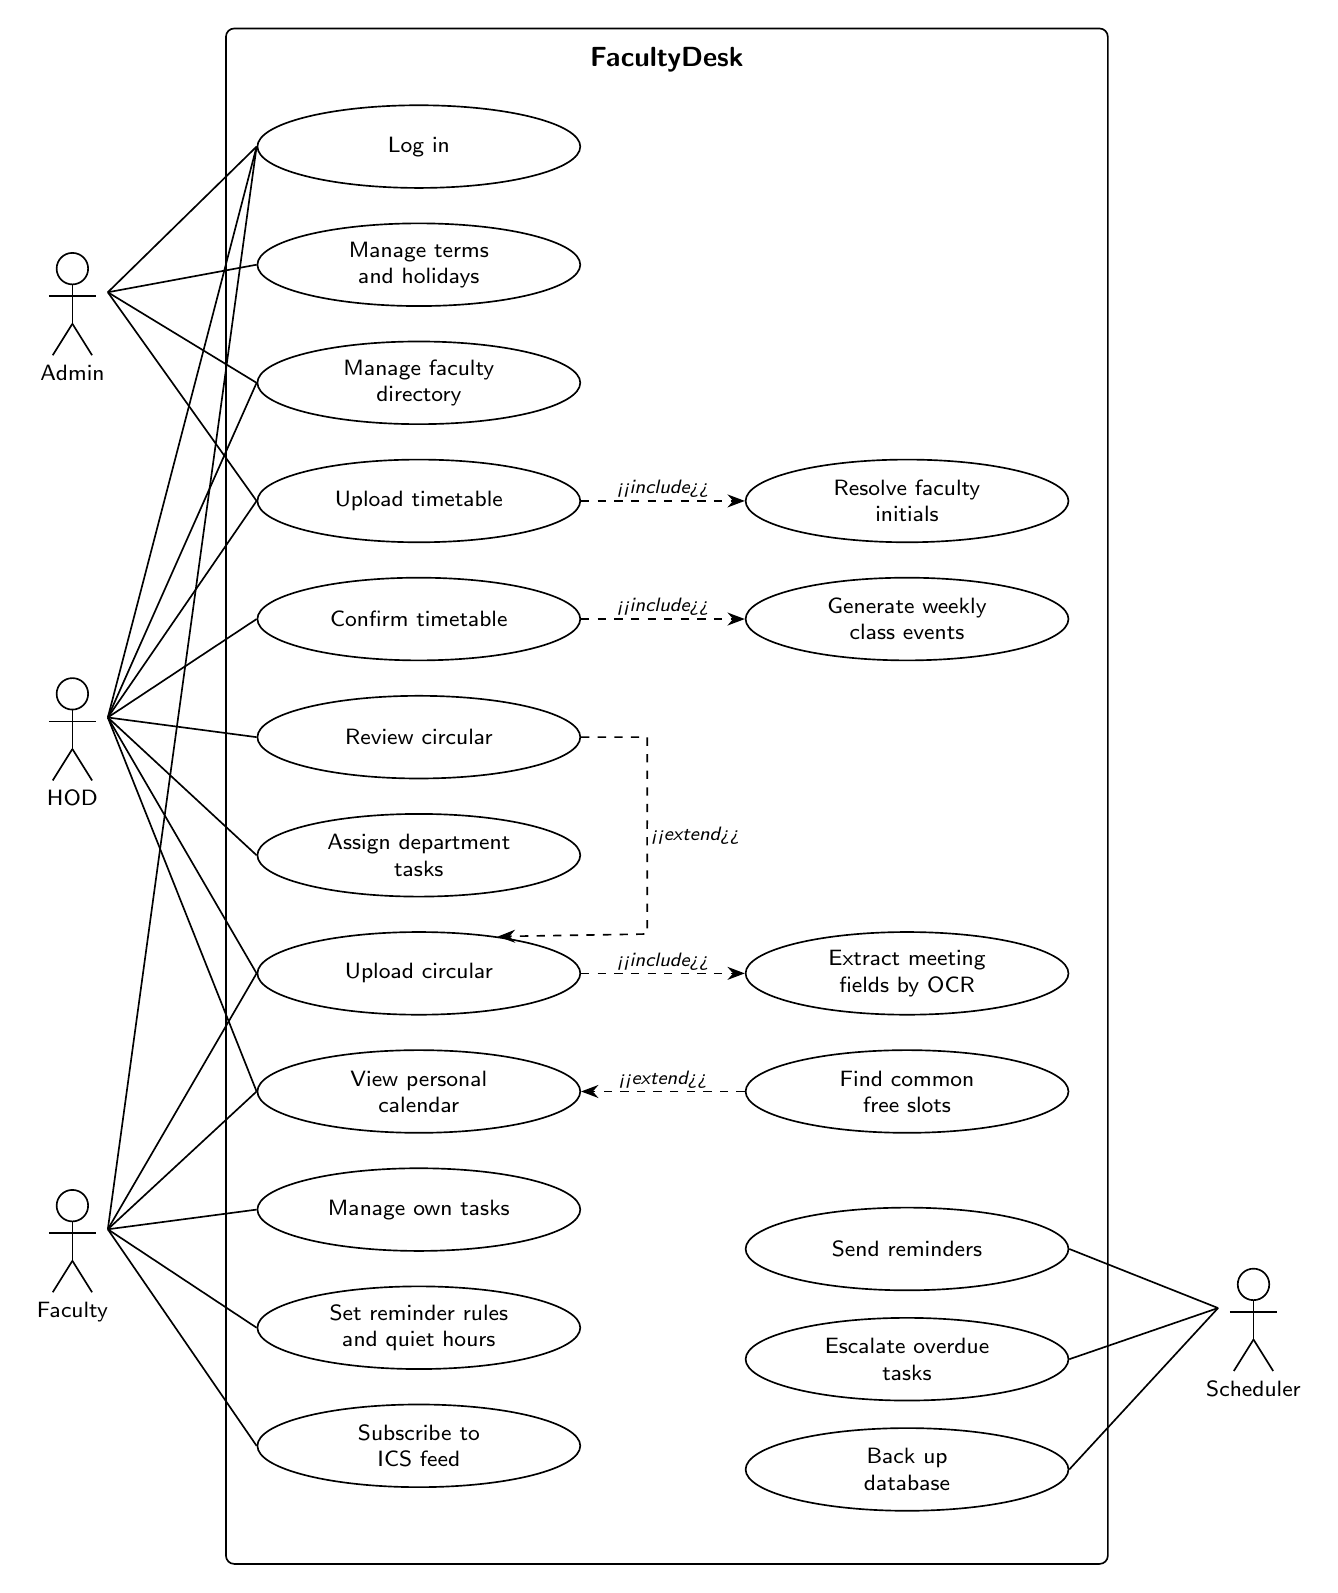
\begin{tikzpicture}[
    uc/.style={ellipse, draw, semithick, fill=ucfill, minimum width=4.1cm, minimum height=1.05cm, align=center, font=\footnotesize, inner sep=1pt},
    assoc/.style={semithick},
    rel/.style={-{Stealth[length=2.2mm]}, dashed, semithick},
    lbl/.style={font=\scriptsize\itshape, fill=white, inner sep=1pt}
  ]
  \draw[semithick, rounded corners=3pt, fill=sysfill] (2.55,-0.4) rectangle (13.75,19.1);
  \node[font=\bfseries] at (8.15,18.7) {FacultyDesk};

  \node[uc] (login) at (5.0,17.6) {Log in};
  \node[uc] (terms) at (5.0,16.1) {Manage terms\\and holidays};
  \node[uc] (dir) at (5.0,14.6) {Manage faculty\\directory};
  \node[uc] (uptt) at (5.0,13.1) {Upload timetable};
  \node[uc] (conftt) at (5.0,11.6) {Confirm timetable};
  \node[uc] (review) at (5.0,10.1) {Review circular};
  \node[uc] (assign) at (5.0,8.6) {Assign department\\tasks};
  \node[uc] (upcirc) at (5.0,7.1) {Upload circular};
  \node[uc] (cal) at (5.0,5.6) {View personal\\calendar};
  \node[uc] (tasks) at (5.0,4.1) {Manage own tasks};
  \node[uc] (prefs) at (5.0,2.6) {Set reminder rules\\and quiet hours};
  \node[uc] (ics) at (5.0,1.1) {Subscribe to\\ICS feed};

  \node[uc] (resolve) at (11.2,13.1) {Resolve faculty\\initials};
  \node[uc] (gen) at (11.2,11.6) {Generate weekly\\class events};
  \node[uc] (ocr) at (11.2,7.1) {Extract meeting\\fields by OCR};
  \node[uc] (free) at (11.2,5.6) {Find common\\free slots};
  \node[uc] (send) at (11.2,3.6) {Send reminders};
  \node[uc] (esc) at (11.2,2.2) {Escalate overdue\\tasks};
  \node[uc] (backup) at (11.2,0.8) {Back up\\database};

  \pic at (0.6,15.3) {actor={Admin}};
  \pic at (0.6,9.9) {actor={HOD}};
  \pic at (0.6,3.4) {actor={Faculty}};
  \pic at (15.6,2.4) {actor={Scheduler}};

  \coordinate (adm) at (1.05,15.75);
  \coordinate (hod) at (1.05,10.35);
  \coordinate (fac) at (1.05,3.85);
  \coordinate (sch) at (15.15,2.85);

  \foreach \u in {login,terms,dir,uptt} \draw[assoc] (adm) -- (\u.west);
  \foreach \u in {login,dir,uptt,conftt,review,assign,upcirc,cal} \draw[assoc] (hod) -- (\u.west);
  \foreach \u in {login,upcirc,cal,tasks,prefs,ics} \draw[assoc] (fac) -- (\u.west);
  \foreach \u in {send,esc,backup} \draw[assoc] (sch) -- (\u.east);

  \draw[rel] (uptt) -- node[lbl, above] {\guill{include}} (resolve);
  \draw[rel] (conftt) -- node[lbl, above] {\guill{include}} (gen);
  \draw[rel] (upcirc) -- node[lbl, above] {\guill{include}} (ocr);
  \draw[rel] (review.east) -- (7.9,10.1) -- node[lbl, right] {\guill{extend}} (7.9,7.6) -- (upcirc.25);
  \draw[rel] (free) -- node[lbl, above] {\guill{extend}} (cal);
\end{tikzpicture}
}
  \caption{FacultyDesk use case diagram}
  \label{fig:usecase}
\end{figure}

\head{Explanation}
\begin{itemize}
  \item \textbf{Actors:} \emph{Admin} manages terms, holidays and the faculty directory. \emph{HOD} uploads and confirms timetables, reviews circulars and assigns tasks. \emph{Faculty} upload circulars, view their calendar, manage tasks, set reminder preferences and subscribe to the ICS feed. \emph{Scheduler} is the background job runner (Celery Beat), a non-human actor.
  \item \textbf{Upload timetable} \guill{include} \textbf{Resolve faculty initials}, because a timetable can never be stored without knowing which teacher each cell refers to.
  \item \textbf{Confirm timetable} \guill{include} \textbf{Generate weekly class events}, because confirmation always creates the classes.
  \item \textbf{Upload circular} \guill{include} \textbf{Extract meeting fields by OCR}, because every uploaded circular is read.
  \item \textbf{Review circular} \guill{extend} \textbf{Upload circular}: review is needed only when the extraction fails the confidence gate.
  \item \textbf{Find common free slots} \guill{extend} \textbf{View personal calendar}: it is an optional step when planning a meeting.
  \item The Scheduler sends reminders, escalates overdue tasks and backs up the database without any human action.
\end{itemize}

\head{Actors and Use Cases Identified}
\needspace{7\baselineskip}
\begin{xltabular}{\textwidth}{|p{2.4cm}|p{2.6cm}|Y|}
\caption{Actors and use cases}\\
\hline
\textbf{Actor} & \textbf{Type} & \textbf{Use cases} \\ \hline
Admin & Primary & Log in, Manage terms and holidays, Manage faculty directory, Upload timetable \\ \hline
HOD & Primary & Log in, Manage faculty directory, Upload timetable, Confirm timetable, Review circular, Assign department tasks, Upload circular, View personal calendar \\ \hline
Faculty & Primary & Log in, Upload circular, View personal calendar, Manage own tasks, Set reminder rules and quiet hours, Subscribe to ICS feed \\ \hline
Scheduler & Supporting (system) & Send reminders, Escalate overdue tasks, Back up database \\ \hline
\end{xltabular}

\ucscenario{UC-01}{Upload and Confirm Timetable}{HOD (primary)}{HOD is logged in; the academic term exists; faculty profiles with initials exist in the department.}{1. HOD selects the term and uploads the timetable file (xlsx, csv or pdf, at most 15 MB).\newline 2. System checks the file type from its first bytes, stores it and starts parsing.\newline 3. System parses the grid, expands merged period cells and resolves each initials token (\emph{include: Resolve faculty initials}).\newline 4. System shows the preview slots and any unresolved tokens.\newline 5. HOD confirms the preview.\newline 6. System saves courses, sections, rooms and slots, and generates the weekly class events (\emph{include: Generate weekly class events}).}{2a. Unsupported file or scanned PDF without text: the upload is rejected with guidance.\newline 4a. Some initials are unresolved or ambiguous: HOD adds an alias in the directory and uploads again.}{Every teacher named in the timetable sees the term's classes on the calendar, without holidays, with reminders planned.}

\ucscenario{UC-02}{Upload and Confirm Meeting Circular}{Faculty or HOD (upload), HOD (review)}{User is logged in; department faculty have initials and aliases.}{1. User uploads a photo, scan or PDF of the circular.\newline 2. System stores it and replies at once; a worker processes it.\newline 3. System reads the text (PDF text layer, or image clean-up and Tesseract OCR) (\emph{include: Extract meeting fields by OCR}).\newline 4. System extracts date, time, venue, title, agenda and attendees.\newline 5. The circular fails the gate and enters the review queue (\emph{extend: Review circular}).\newline 6. HOD corrects any field and confirms.\newline 7. System creates a MEETING event for every attendee and plans their reminders.}{3a. File or OCR error: circular becomes FAILED and can be processed again.\newline 5a. All fields pass the gate and the department allows automatic confirmation: the meeting is created without review.\newline 6a. HOD rejects the circular: it becomes REJECTED and no event is created.}{Each named attendee sees the meeting and receives reminders at their chosen lead times.}

\ucscenario{UC-03}{Send Reminders}{Scheduler (primary), Faculty (receiver)}{Pending reminders exist with a fire time in the past; the user has an e-mail address or a push subscription.}{1. Every 30 seconds the Scheduler starts the dispatch job.\newline 2. System claims up to 100 due reminders, locking them so no other worker takes them.\newline 3. For each reminder, the system builds the message from the event or task.\newline 4. The reminder is sent by e-mail or web push and marked SENT.}{3a. The task is already completed: the reminder is cancelled.\newline 4a. Sending fails: the reminder is retried later, up to five attempts, then marked FAILED.}{Each reminder is delivered at most once; the Admin can see delivery counts and failures.}

\ucscenario{UC-04}{Assign and Complete Documentation Task}{HOD (assign), Faculty (complete)}{HOD and faculty accounts exist; task templates are seeded.}{1. HOD picks a template (for example IA marks upload) or writes a task, sets a deadline and importance.\newline 2. HOD assigns it to one teacher, a group or the whole department.\newline 3. System creates one task per assignee, a DEADLINE event on each calendar, and alerts at 72 h, 24 h and 2 h before the deadline.\newline 4. Faculty see the task ranked by priority and mark it complete.\newline 5. System cancels the remaining alerts and updates the HOD dashboard.}{4a. Deadline passes: daily overdue alerts start and the HOD receives an escalation summary.\newline 5a. Faculty reopen the task: future alerts are scheduled again.}{The HOD dashboard shows the completion rate and overdue count per teacher.}

\head{Conclusion}
The use case diagram captures every service of FacultyDesk and who uses it. The \guill{include} relation models mandatory steps such as initials resolution and OCR, and \guill{extend} models optional steps such as review and free-slot finding.

\subsection{Class Diagram}

\theory{Theory}
A class diagram is a structural UML diagram that shows the classes of a system, their attributes and operations, and the relationships between them. It is the main diagram of object-oriented design and maps directly to code. A class is drawn as a rectangle with three compartments: name, attributes and operations. Visibility is shown with \textbf{+} public, \textbf{--} private, \textbf{\#} protected and \textbf{\textasciitilde} package.

\theory{Relationships Between Classes}
\needspace{7\baselineskip}
\begin{xltabular}{\textwidth}{|p{3cm}|>{\centering\arraybackslash}p{3cm}|Y|}
\caption{Class relationship notation}\\
\hline
\textbf{Relationship} & \textbf{Symbol} & \textbf{Example in FacultyDesk} \\ \hline
Association & \symline & FacultyProfile belongs to a Department. \\ \hline
Aggregation & \symagg & CompositeNotifier has an EmailNotifier and a WebPushNotifier. \\ \hline
Composition & \symcomp & Event owns its EventAttendees; AcademicTerm owns its Holidays. \\ \hline
Generalization & \symgen & XlsxTimetableParser is a TimetableParser. \\ \hline
Realization & \symreal & SystemClock implements the Clock protocol. \\ \hline
Dependency & \symdep & A Circular creates an Event when confirmed. \\ \hline
\end{xltabular}

\theory{Multiplicity}
\begin{table}[H]
\centering
\begin{tabular}{|p{2.6cm}|p{6.6cm}|}
\hline
\textbf{Notation} & \textbf{Meaning} \\ \hline
1 & Exactly one \\ \hline
0..1 & Zero or one \\ \hline
* or 0..* & Zero or more \\ \hline
1..* & One or more \\ \hline
\end{tabular}
\caption{Multiplicity notation}
\end{table}

\begin{figure}[!htbp]
  \centering
  \resizebox{\textwidth}{!}{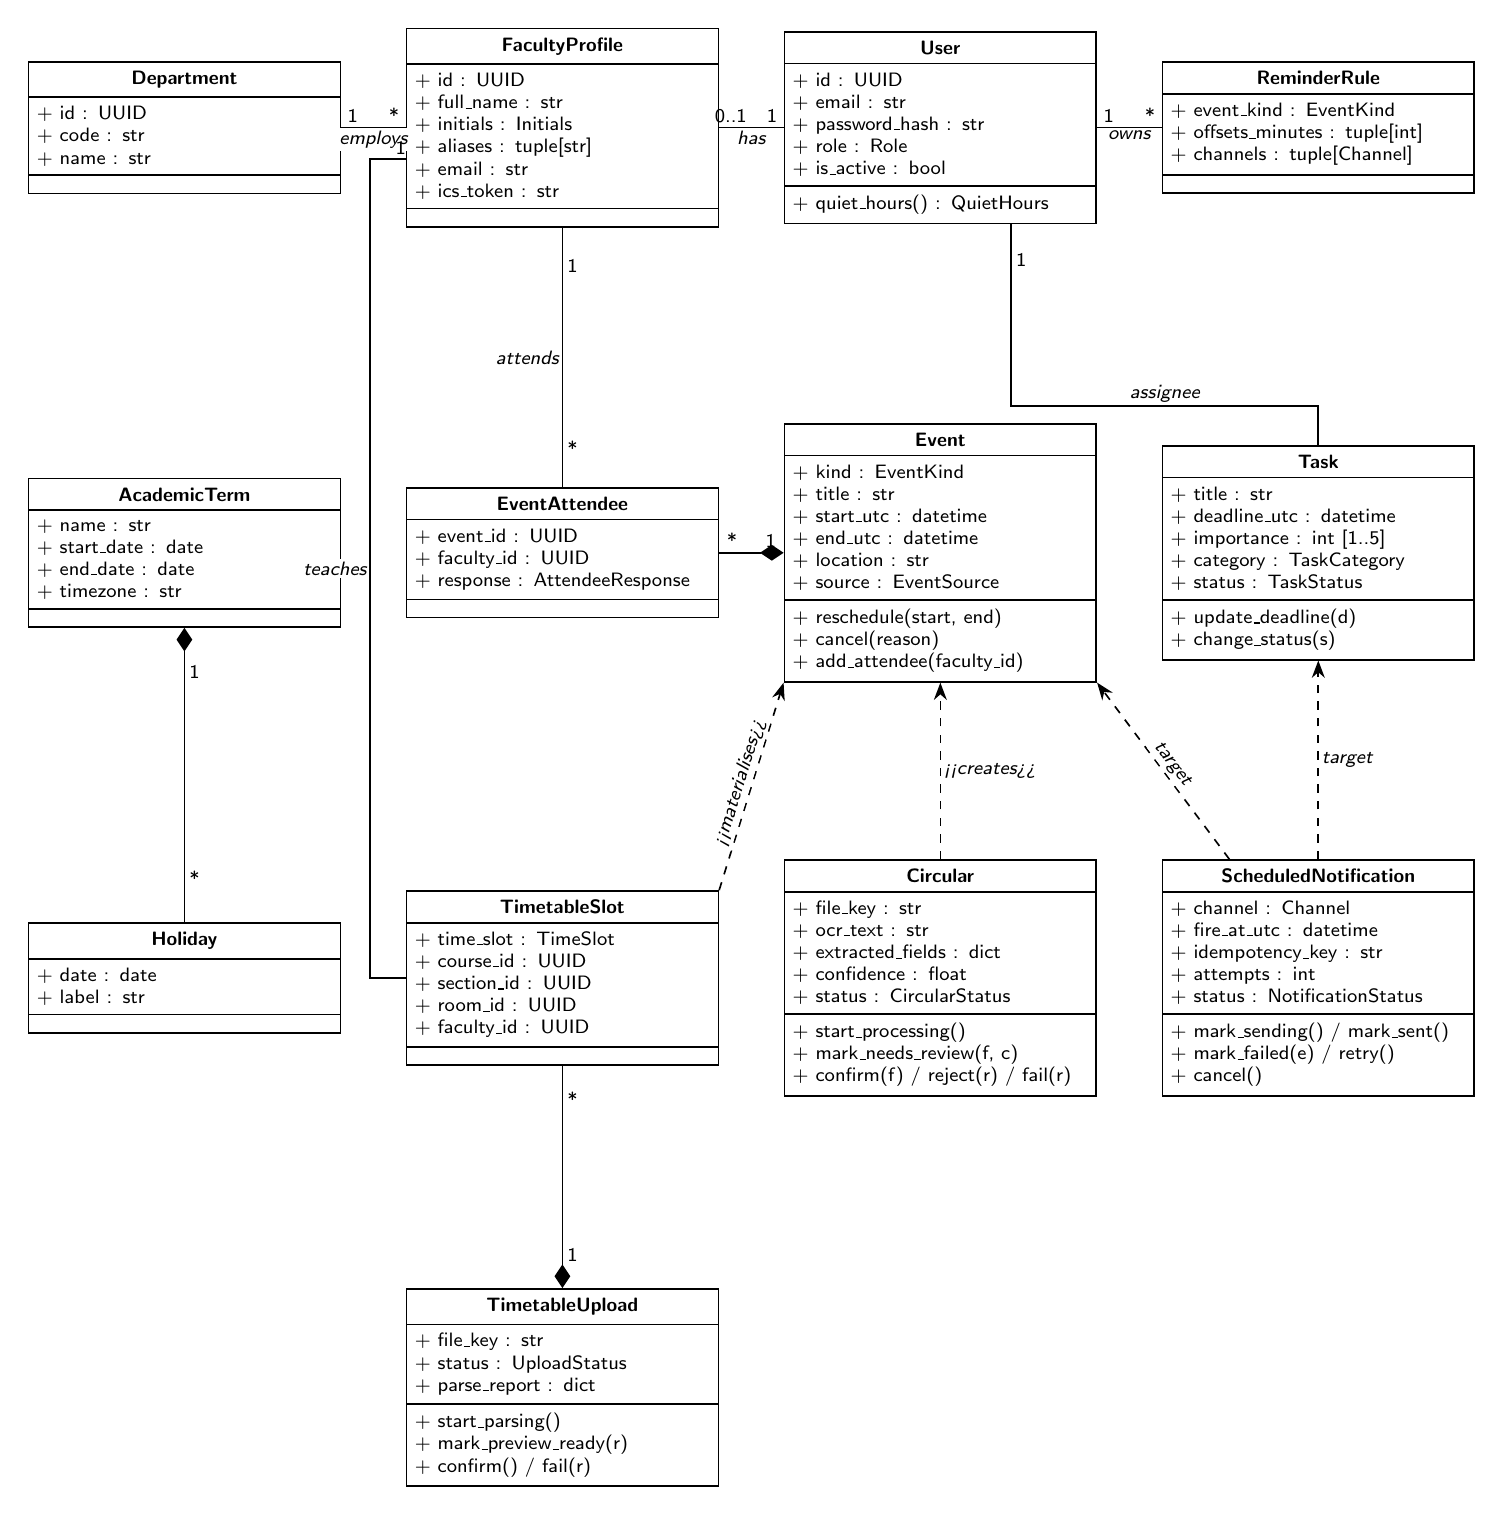
\begin{tikzpicture}[
    assoc/.style={semithick},
    comp/.style={semithick, {Diamond[length=3mm, width=2mm, fill=black]}-},
    dep/.style={semithick, dashed, -{Stealth[length=2.2mm]}},
    m/.style={font=\scriptsize, inner sep=1.5pt},
    lbl/.style={font=\scriptsize\itshape, fill=white, inner sep=1pt}
  ]
  \umlclass{dept}{0,0}{Department}{
    + id : UUID\\
    + code : str\\
    + name : str}{}
  \umlclass{fp}{4.8,0}{FacultyProfile}{
    + id : UUID\\
    + full\_name : str\\
    + initials : Initials\\
    + aliases : tuple[str]\\
    + email : str\\
    + ics\_token : str}{}
  \umlclass{user}{9.6,0}{User}{
    + id : UUID\\
    + email : str\\
    + password\_hash : str\\
    + role : Role\\
    + is\_active : bool}{
    + quiet\_hours() : QuietHours}
  \umlclass{rule}{14.4,0}{ReminderRule}{
    + event\_kind : EventKind\\
    + offsets\_minutes : tuple[int]\\
    + channels : tuple[Channel]}{}

  \umlclass{term}{0,-5.4}{AcademicTerm}{
    + name : str\\
    + start\_date : date\\
    + end\_date : date\\
    + timezone : str}{}
  \umlclass{att}{4.8,-5.4}{EventAttendee}{
    + event\_id : UUID\\
    + faculty\_id : UUID\\
    + response : AttendeeResponse}{}
  \umlclass{event}{9.6,-5.4}{Event}{
    + kind : EventKind\\
    + title : str\\
    + start\_utc : datetime\\
    + end\_utc : datetime\\
    + location : str\\
    + source : EventSource}{
    + reschedule(start, end)\\
    + cancel(reason)\\
    + add\_attendee(faculty\_id)}
  \umlclass{task}{14.4,-5.4}{Task}{
    + title : str\\
    + deadline\_utc : datetime\\
    + importance : int [1..5]\\
    + category : TaskCategory\\
    + status : TaskStatus}{
    + update\_deadline(d)\\
    + change\_status(s)}

  \umlclass{hol}{0,-10.8}{Holiday}{
    + date : date\\
    + label : str}{}
  \umlclass{slot}{4.8,-10.8}{TimetableSlot}{
    + time\_slot : TimeSlot\\
    + course\_id : UUID\\
    + section\_id : UUID\\
    + room\_id : UUID\\
    + faculty\_id : UUID}{}
  \umlclass{circ}{9.6,-10.8}{Circular}{
    + file\_key : str\\
    + ocr\_text : str\\
    + extracted\_fields : dict\\
    + confidence : float\\
    + status : CircularStatus}{
    + start\_processing()\\
    + mark\_needs\_review(f, c)\\
    + confirm(f) / reject(r) / fail(r)}
  \umlclass{notif}{14.4,-10.8}{ScheduledNotification}{
    + channel : Channel\\
    + fire\_at\_utc : datetime\\
    + idempotency\_key : str\\
    + attempts : int\\
    + status : NotificationStatus}{
    + mark\_sending() / mark\_sent()\\
    + mark\_failed(e) / retry()\\
    + cancel()}

  \umlclass{upload}{4.8,-16.0}{TimetableUpload}{
    + file\_key : str\\
    + status : UploadStatus\\
    + parse\_report : dict}{
    + start\_parsing()\\
    + mark\_preview\_ready(r)\\
    + confirm() / fail(r)}

  \draw[assoc] (dept) -- node[m, above, pos=0.18] {1} node[m, above, pos=0.82] {*} node[lbl, below] {employs} (fp);
  \draw[assoc] (user) -- node[m, above, pos=0.18] {1} node[m, above, pos=0.82] {0..1} node[lbl, below] {has} (fp);
  \draw[assoc] (user) -- node[m, above, pos=0.18] {1} node[m, above, pos=0.82] {*} node[lbl, below] {owns} (rule);
  \draw[comp] (term) -- node[m, right, pos=0.15] {1} node[m, right, pos=0.85] {*} (hol);
  \draw[assoc] (fp) -- node[m, right, pos=0.15] {1} node[m, right, pos=0.85] {*} node[lbl, left] {attends} (att);
  \draw[comp] (event) -- node[m, above, pos=0.2] {1} node[m, above, pos=0.8] {*} (att);
  \draw[comp] (upload) -- node[m, right, pos=0.15] {1} node[m, right, pos=0.85] {*} (slot);
  \draw[assoc] (slot.west) -- ++(-0.45,0) |- node[lbl, pos=0.25, left] {teaches} node[m, above, pos=0.93] {1} ([yshift=-4mm]fp.west);
  \draw[dep] (slot.north east) -- node[lbl, sloped, above] {\guill{materialises}} (event.south west);
  \draw[dep] (circ) -- node[lbl, right] {\guill{creates}} (event);
  \draw[dep] (notif) -- node[lbl, sloped, above] {target} (event.south east);
  \draw[dep] (notif) -- node[lbl, right] {target} (task);
  \draw[assoc] (task.north) -- ++(0,0.5) -| node[m, right, pos=0.9] {1} node[lbl, pos=0.25, above] {assignee} ([xshift=9mm]user.south);
\end{tikzpicture}
}
  \caption{FacultyDesk domain class diagram}
  \label{fig:classdomain}
\end{figure}

\head{Classes Identified}
{\small
\begin{xltabular}{\textwidth}{|p{3.3cm}|Y|Y|}
\caption{Domain classes with attributes and operations}\\
\hline
\textbf{Class} & \textbf{Attributes} & \textbf{Operations / rules} \\ \hline
User & email, password\_hash, role, is\_active, quiet hours & quiet\_hours() \\ \hline
FacultyProfile & full\_name, initials, aliases, email, phone, ics\_token & initials must be 2--5 capital letters \\ \hline
Department & code, name & -- \\ \hline
AcademicTerm & name, start\_date, end\_date, timezone & owns Holidays \\ \hline
Holiday & date, label & -- \\ \hline
TimetableUpload & file\_key, status, parse\_report & start\_parsing(), mark\_preview\_ready(), confirm(), fail() \\ \hline
TimetableSlot & time\_slot, course, section, room, faculty & -- \\ \hline
Event & kind, title, start\_utc, end\_utc, location, source & reschedule(), cancel(), add\_attendee() \\ \hline
EventAttendee & event\_id, faculty\_id, response & -- \\ \hline
Circular & file\_key, ocr\_text, extracted\_fields, confidence, status & start\_processing(), mark\_needs\_review(), confirm(), reject(), fail() \\ \hline
ScheduledNotification & channel, fire\_at\_utc, idempotency\_key, attempts, status & mark\_sending(), mark\_sent(), mark\_failed(), retry(), cancel() \\ \hline
ReminderRule & event\_kind, offsets\_minutes, channels & offsets cannot be negative \\ \hline
Task & title, deadline\_utc, importance (1--5), category, status & update\_deadline(), change\_status() \\ \hline
\end{xltabular}}

\head{Relationships}
\begin{itemize}
  \item \textbf{FacultyProfile} is the central class: it belongs to a \textbf{Department}, is linked to one \textbf{User} account, teaches \textbf{TimetableSlot}s and attends \textbf{Event}s through \textbf{EventAttendee}.
  \item \textbf{Composition:} a \textbf{TimetableUpload} owns its slots, an \textbf{Event} owns its attendees, and an \textbf{AcademicTerm} owns its holidays; the parts have no meaning without the whole.
  \item \textbf{Event} is one class for classes, meetings and deadlines; its \texttt{kind} attribute tells them apart, so clash detection, reminders and the ICS feed treat them the same way.
  \item A confirmed \textbf{TimetableSlot} is \emph{materialised} into weekly CLASS events, and a confirmed \textbf{Circular} \emph{creates} one MEETING event.
  \item A \textbf{ScheduledNotification} targets an \textbf{Event} or a \textbf{Task}; a \textbf{Task} has one assignee \textbf{User}.
\end{itemize}

\head{Conclusion}
The class diagram shows that the business rules live in the classes themselves: each class validates its own data and controls its own status changes, which is the basis of the object-oriented design.

\subsection{Sequence Diagrams}

\theory{Theory}
A sequence diagram is an interaction diagram that shows how objects communicate by exchanging messages in time order. Time flows from top to bottom. Each participant has a lifeline; messages are arrows between lifelines; combined fragments such as \texttt{alt} (alternatives) and \texttt{loop} (repetition) group messages.

\theory{Sequence Diagram Notation}
\needspace{7\baselineskip}
\begin{xltabular}{\textwidth}{|p{3.2cm}|>{\centering\arraybackslash}p{3cm}|Y|}
\caption{Sequence diagram notation}\\
\hline
\textbf{Element} & \textbf{Symbol} & \textbf{Meaning} \\ \hline
Lifeline & \symlifeline & An object taking part in the interaction. \\ \hline
Synchronous message & \symsync & The sender waits for the reply. \\ \hline
Asynchronous message & \symasync & The sender continues without waiting. \\ \hline
Reply message & \symreply & Return of control or a value. \\ \hline
Self message & -- & A message an object sends to itself. \\ \hline
alt / loop fragment & -- & Alternative paths with guards / repeated messages. \\ \hline
\end{xltabular}

\begin{figure}[!htbp]
  \centering
  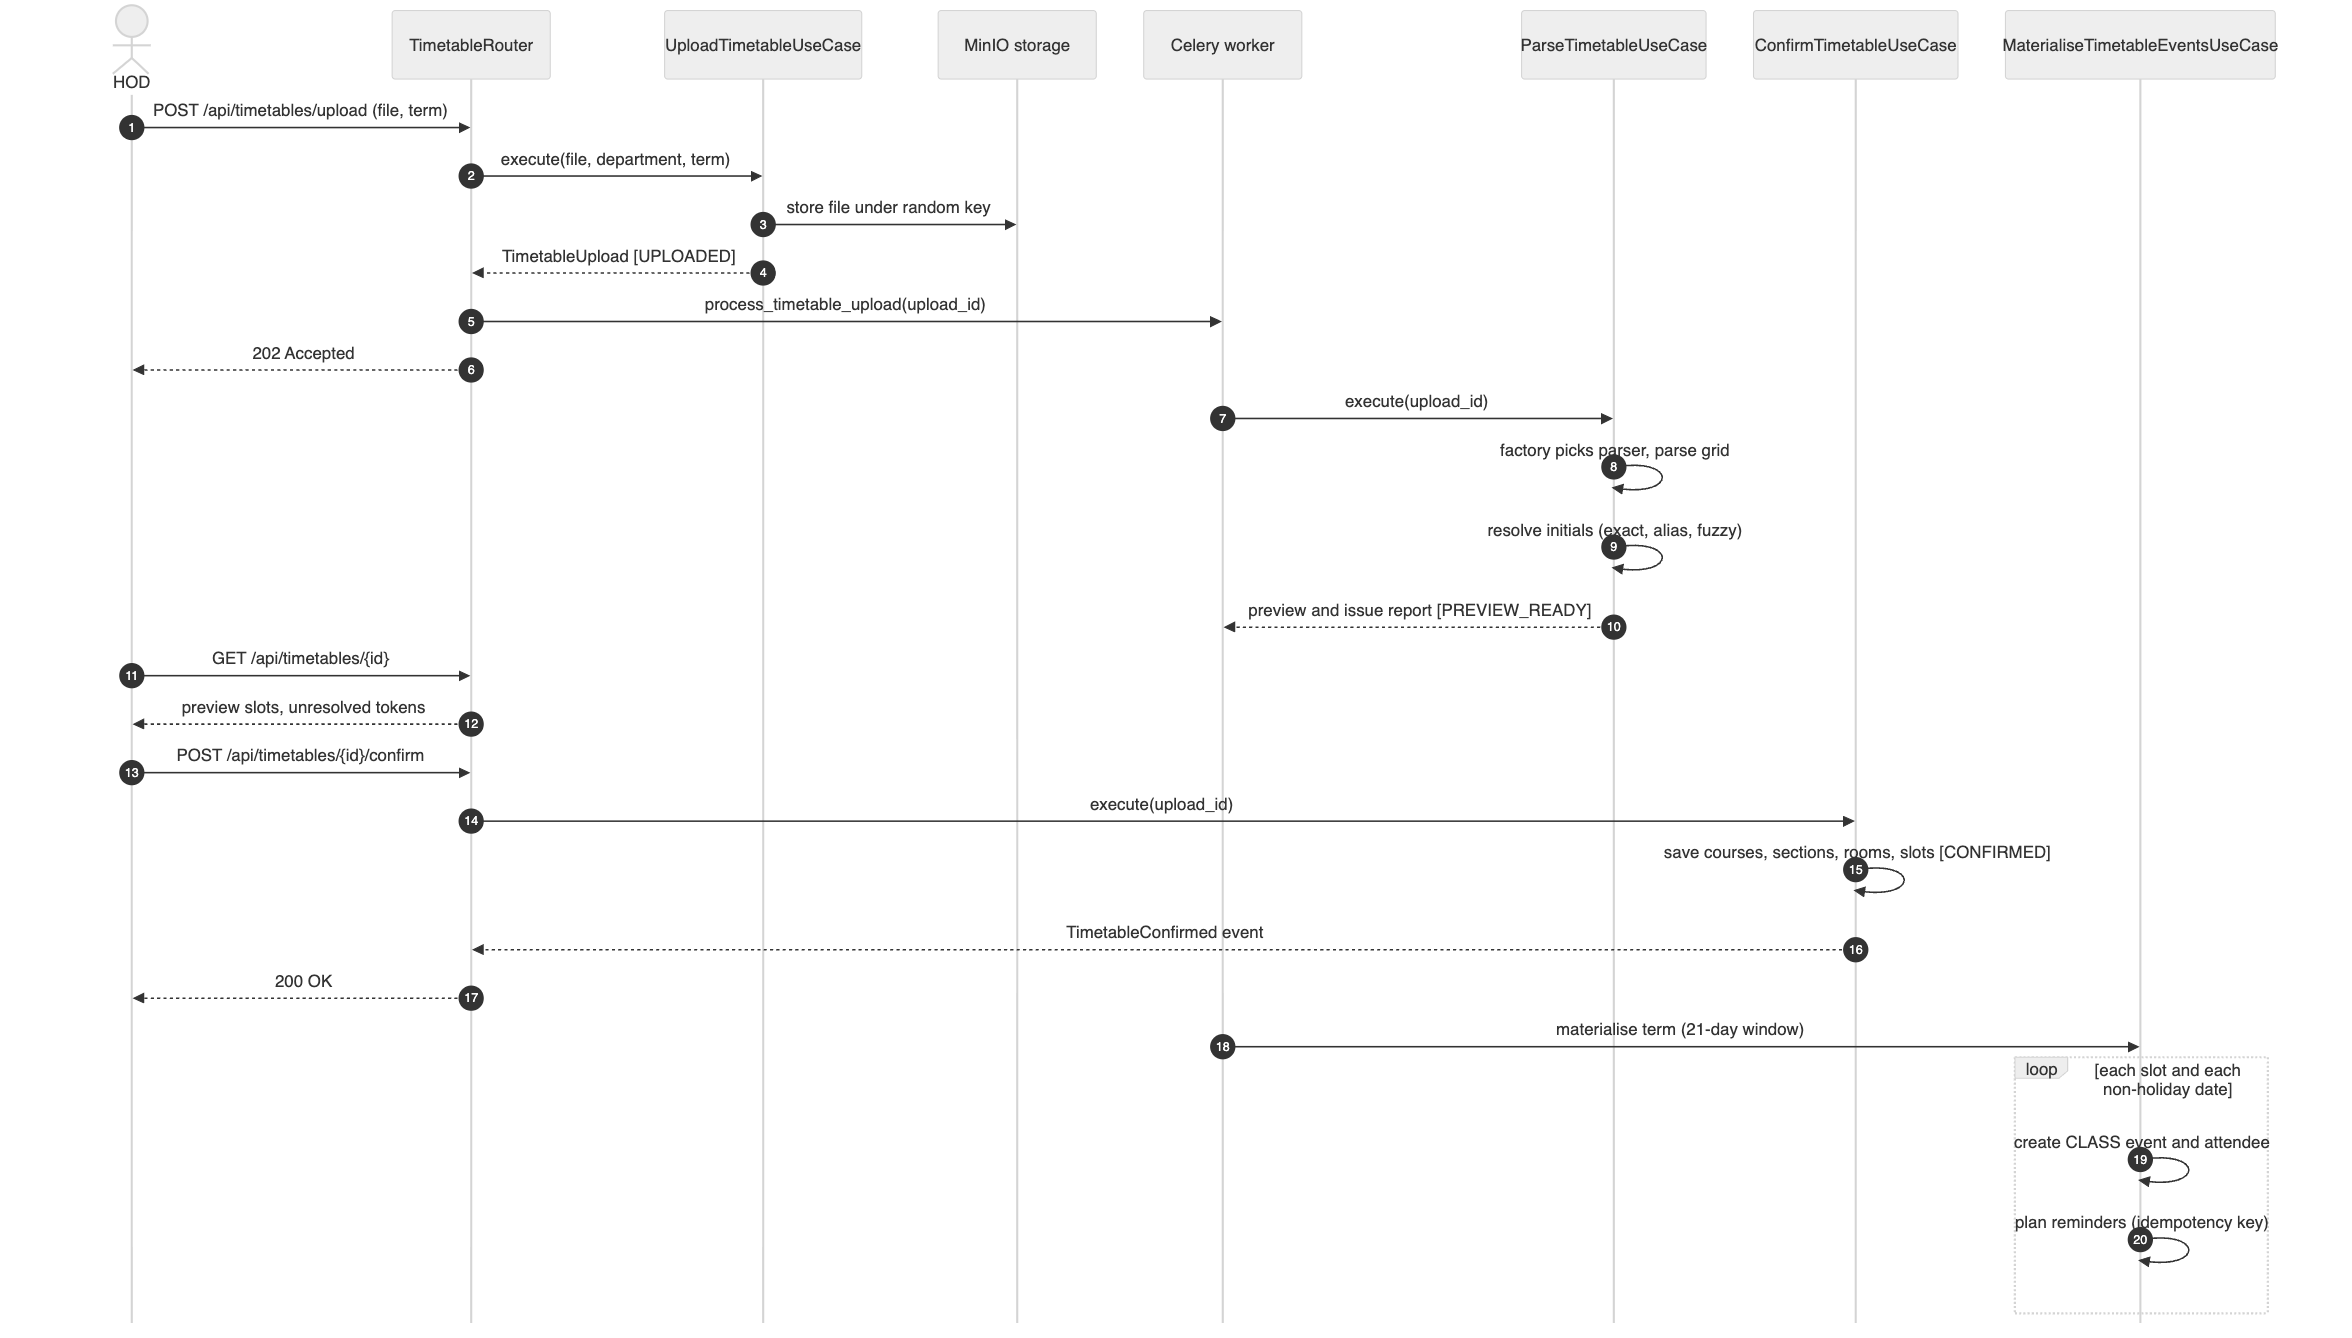
\includegraphics[width=\textwidth]{figures/seq_timetable.png}
  \caption{Sequence diagram: timetable upload and class generation}
  \label{fig:seqtt}
\end{figure}

\head{Explanation}
\begin{enumerate}
  \item The HOD uploads the file (1). The router passes it to \texttt{UploadTimetableUseCase}, which stores it and returns a \texttt{TimetableUpload} in state UPLOADED (2--4).
  \item The router hands parsing to a Celery worker and replies \texttt{202 Accepted} at once (5--6), so the web request stays short.
  \item The worker runs \texttt{ParseTimetableUseCase}: the factory picks the parser and the initials are resolved (7--10).
  \item The HOD reads the preview (11--12) and confirms (13). \texttt{ConfirmTimetableUseCase} saves the slots and raises a \texttt{TimetableConfirmed} event (14--17).
  \item The worker then expands each slot over the term in a \texttt{loop}, creating CLASS events and planning reminders (18--20).
\end{enumerate}

\begin{figure}[!htbp]
  \centering
  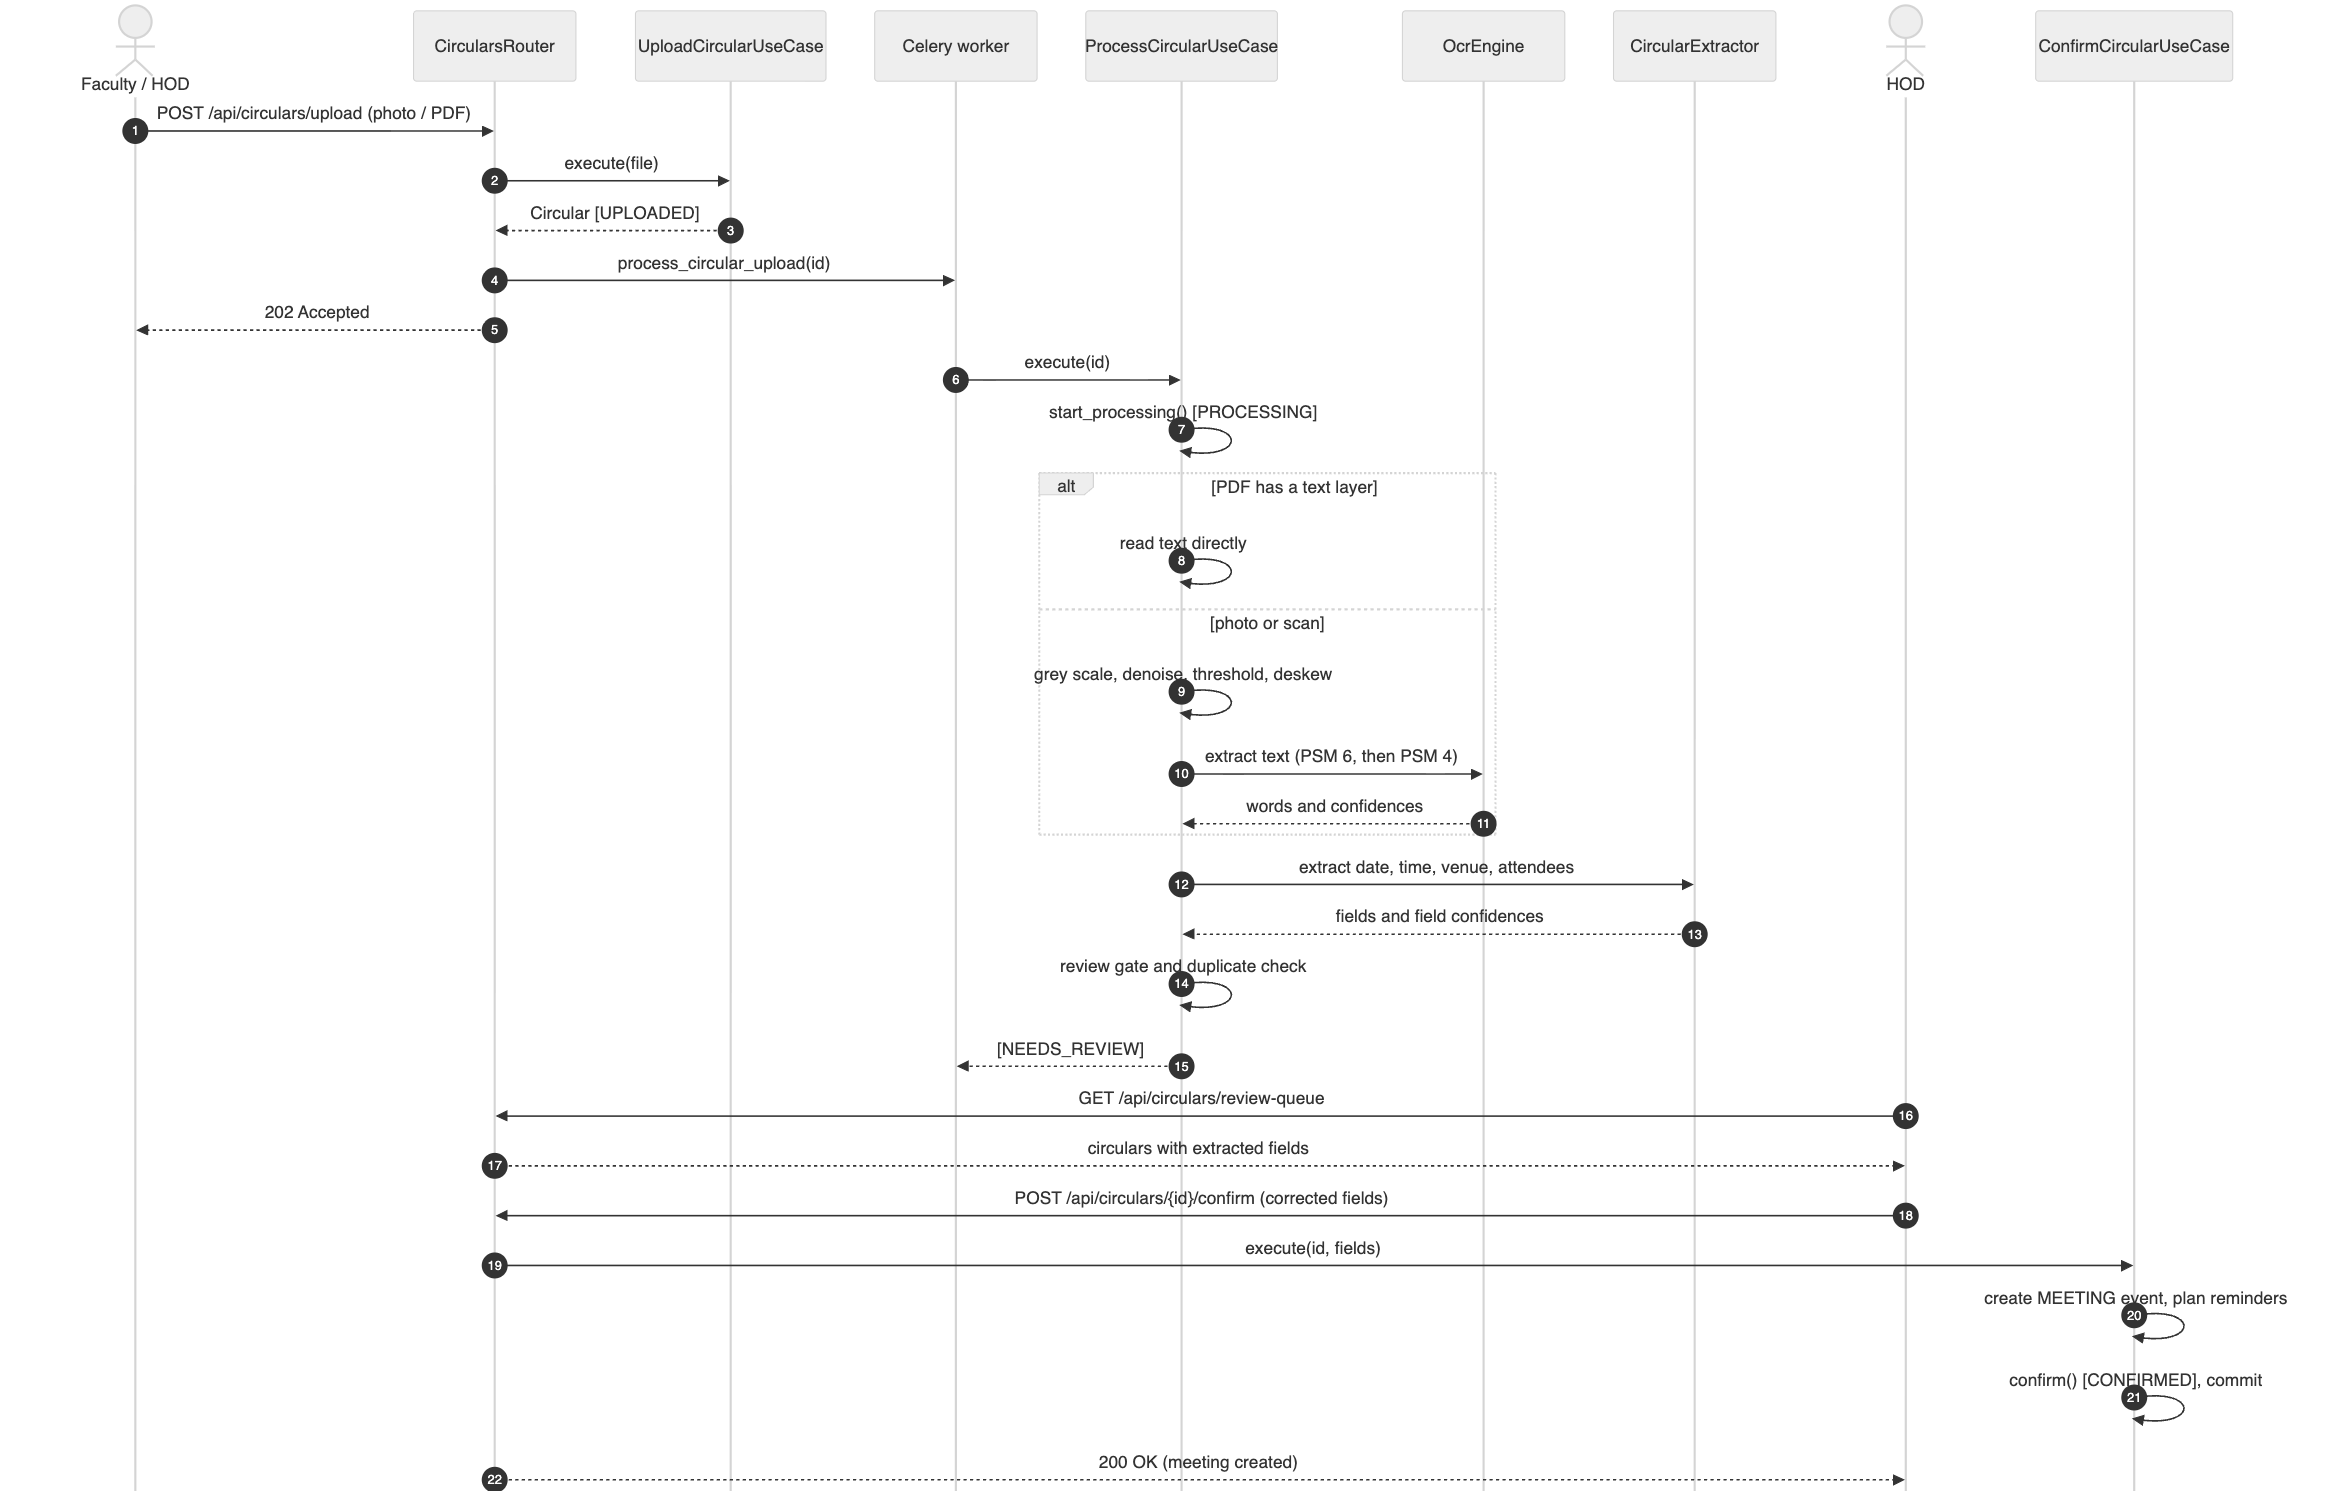
\includegraphics[width=\textwidth]{figures/seq_circular.png}
  \caption{Sequence diagram: circular upload, OCR, review and confirmation}
  \label{fig:seqcirc}
\end{figure}

\head{Explanation}
\begin{enumerate}
  \item Upload is answered immediately (1--5); processing runs in a worker (6--7).
  \item The \texttt{alt} fragment shows the two reading paths: a PDF with a text layer is read directly (8); a photo or scan is cleaned and read by \texttt{OcrEngine} with two page-segmentation modes (9--11).
  \item \texttt{CircularExtractor} returns the fields with a confidence for each (12--13), and the review gate puts the circular in NEEDS\_REVIEW (14--15).
  \item The HOD opens the review queue, corrects the fields and confirms (16--19); \texttt{ConfirmCircularUseCase} creates the meeting, plans reminders and commits (20--22).
\end{enumerate}

\begin{figure}[!htbp]
  \centering
  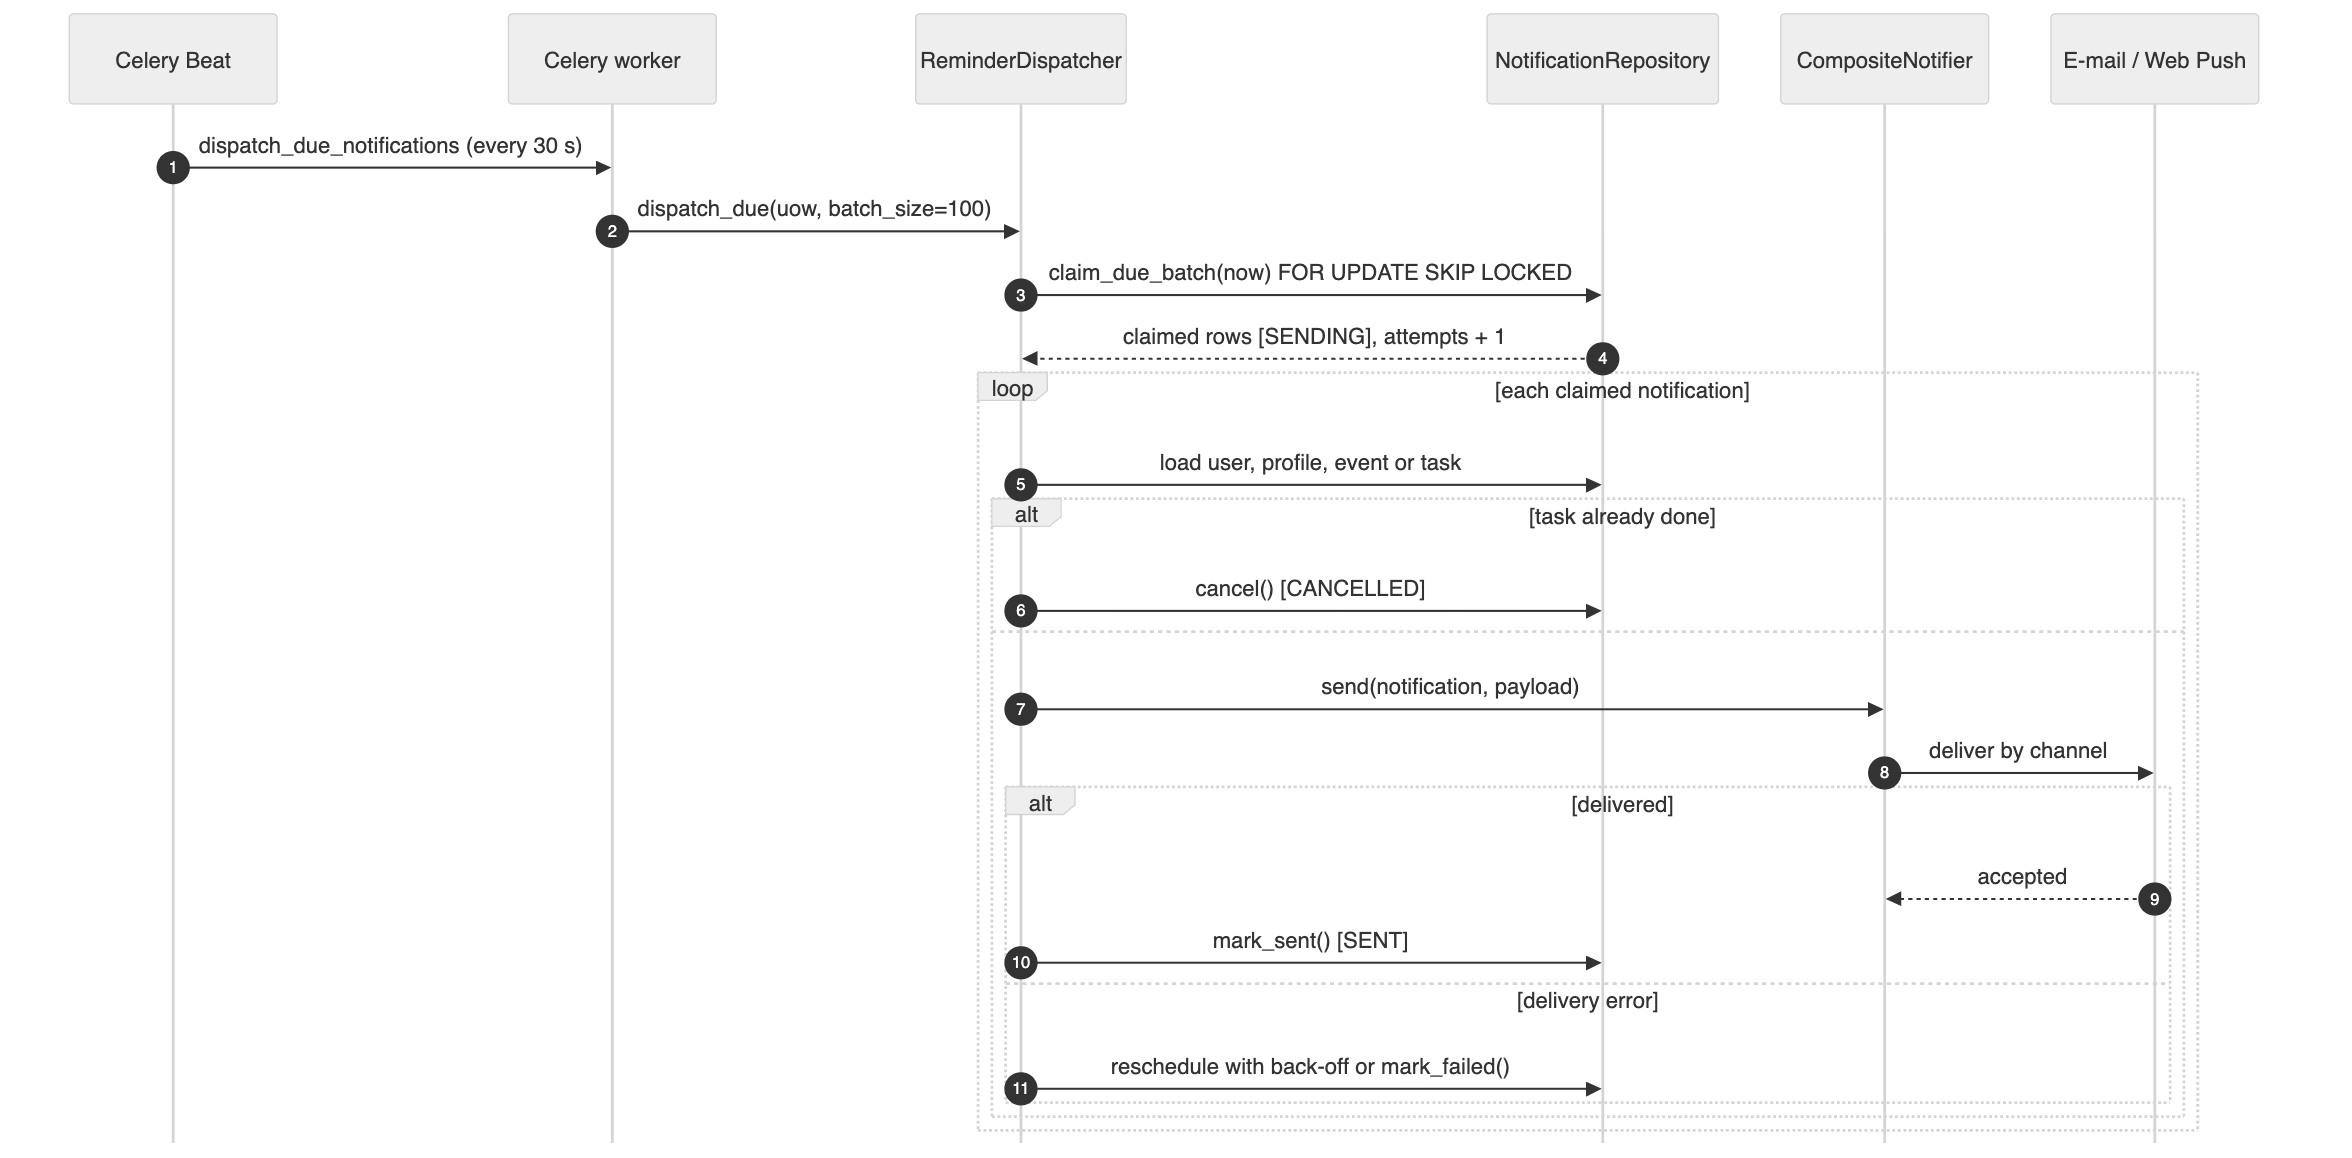
\includegraphics[width=0.95\textwidth]{figures/seq_dispatch.png}
  \caption{Sequence diagram: periodic reminder dispatch}
  \label{fig:seqdisp}
\end{figure}

\head{Explanation}
\begin{enumerate}
  \item Every 30 seconds Celery Beat starts the dispatch job (1--2).
  \item The dispatcher claims up to 100 due reminders with \texttt{SELECT ... FOR UPDATE SKIP LOCKED}, so two workers can never claim the same row, and marks them SENDING (3--4).
  \item For each reminder it loads the user and the event or task (5). If the task is already done, the reminder is cancelled; otherwise it is sent through \texttt{CompositeNotifier}, which chooses e-mail or web push (6--8).
  \item A successful send is marked SENT; a failed one is rescheduled with back-off or marked FAILED after five attempts (9--11).
\end{enumerate}

\head{Conclusion}
The three sequence diagrams show the time order of the main flows and the design decision behind them: slow work is moved to workers so that users always get an immediate answer.

\subsection{Collaboration (Communication) Diagram}

\theory{Theory}
A collaboration diagram, called a communication diagram in UML 2, shows the same interaction as a sequence diagram but arranges the objects by their links instead of by time. Messages are written along the links and numbered in nested decimal form (1, 1.1, 1.1.1), so the order and the call nesting are still visible.

\needspace{7\baselineskip}
\begin{xltabular}{\textwidth}{|p{3.2cm}|Y|Y|}
\caption{Sequence versus collaboration diagram}\\
\hline
\textbf{Point} & \textbf{Sequence diagram} & \textbf{Collaboration diagram} \\ \hline
Emphasis & Time order of messages & Structural links between objects \\ \hline
Layout & Lifelines from left to right, time downwards & Objects placed freely, joined by links \\ \hline
Message order & Vertical position & Decimal numbers (1, 1.1, 1.1.1) \\ \hline
Best for & Long flows with many steps & Seeing which objects work together \\ \hline
\end{xltabular}

\begin{figure}[!htbp]
  \centering
  \resizebox{\textwidth}{!}{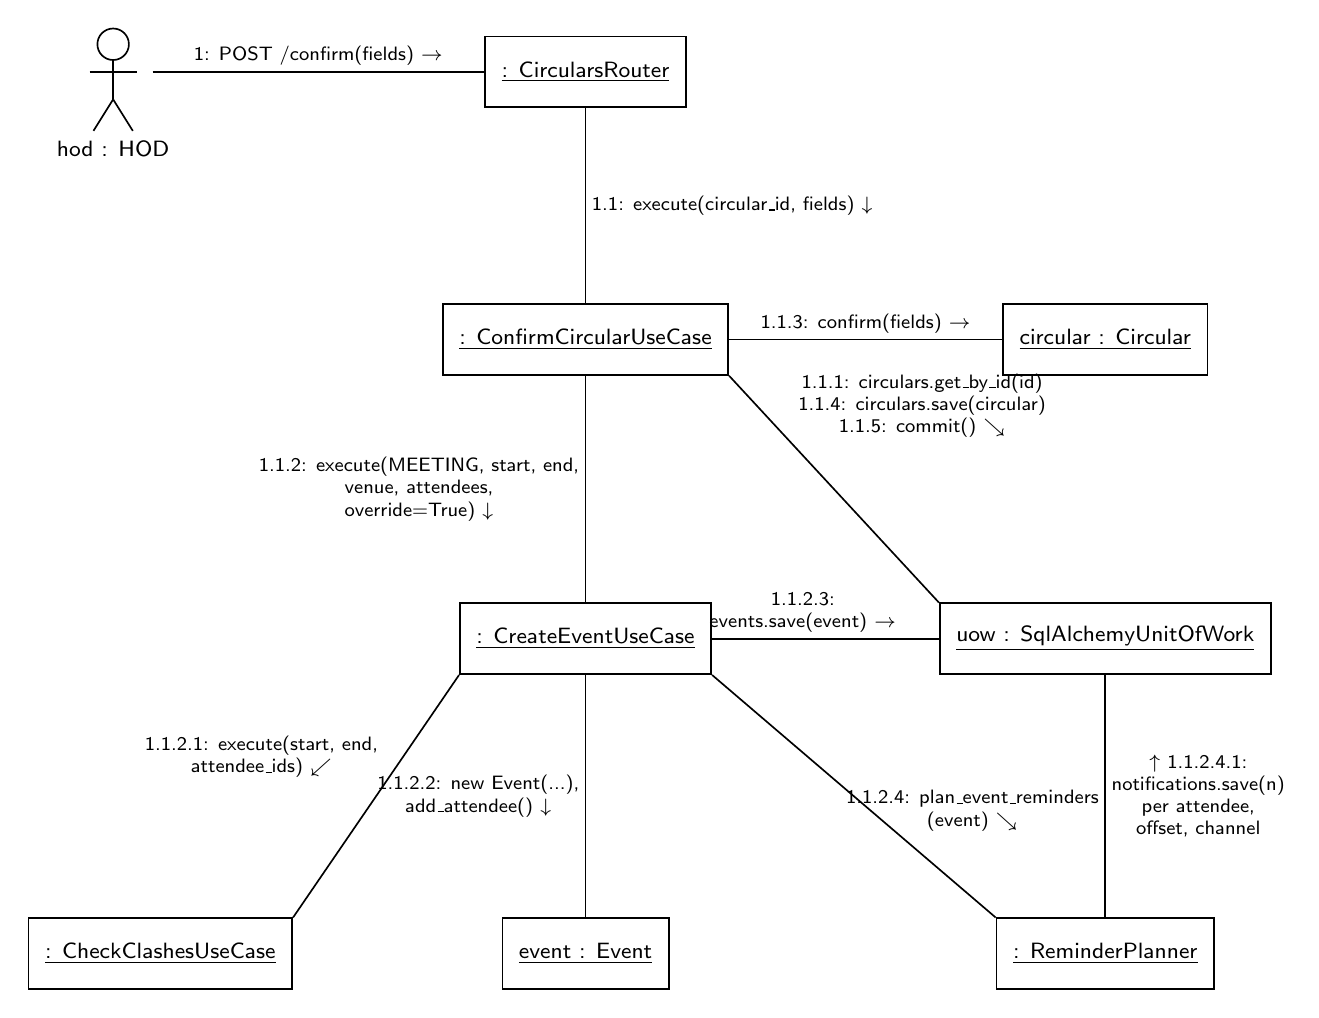
\begin{tikzpicture}[
    obj/.style={rectangle, draw, semithick, fill=white, font=\footnotesize, minimum height=0.9cm, inner xsep=6pt, align=center},
    link/.style={semithick},
    msg/.style={font=\scriptsize, inner sep=2pt, align=center}
  ]
  \pic at (0,-0.4) {actor={hod : HOD}};
  \node[obj] (router) at (6.0,0) {\underline{: CircularsRouter}};
  \node[obj] (confirm) at (6.0,-3.4) {\underline{: ConfirmCircularUseCase}};
  \node[obj] (circ) at (12.6,-3.4) {\underline{circular : Circular}};
  \node[obj] (create) at (6.0,-7.2) {\underline{: CreateEventUseCase}};
  \node[obj] (uow) at (12.6,-7.2) {\underline{uow : SqlAlchemyUnitOfWork}};
  \node[obj] (clash) at (0.6,-11.2) {\underline{: CheckClashesUseCase}};
  \node[obj] (event) at (6.0,-11.2) {\underline{event : Event}};
  \node[obj] (planner) at (12.6,-11.2) {\underline{: ReminderPlanner}};

  \draw[link] (0.5,0) -- node[msg, above] {1: POST /confirm(fields) $\rightarrow$} (router);
  \draw[link] (router) -- node[msg, right] {1.1: execute(circular\_id, fields) $\downarrow$} (confirm);
  \draw[link] (confirm) -- node[msg, above] {1.1.3: confirm(fields) $\rightarrow$} (circ);
  \draw[link] (confirm.south east) -- node[msg, above right, pos=0.3] {1.1.1: circulars.get\_by\_id(id)\\1.1.4: circulars.save(circular)\\1.1.5: commit() $\searrow$} (uow.north west);
  \draw[link] (confirm) -- node[msg, left] {1.1.2: execute(MEETING, start, end,\\venue, attendees,\\override=True) $\downarrow$} (create);
  \draw[link] (create) -- node[msg, above, pos=0.4] {1.1.2.3:\\events.save(event) $\rightarrow$} (uow);
  \draw[link] (create.south west) -- node[msg, above left, pos=0.45] {1.1.2.1: execute(start, end,\\attendee\_ids) $\swarrow$} (clash.north east);
  \draw[link] (create) -- node[msg, left] {1.1.2.2: new Event(...),\\add\_attendee() $\downarrow$} (event);
  \draw[link] (create.south east) -- node[msg, below right, pos=0.45] {1.1.2.4: plan\_event\_reminders\\(event) $\searrow$} (planner.north west);
  \draw[link] (planner) -- node[msg, right] {$\uparrow$ 1.1.2.4.1:\\notifications.save(n)\\per attendee,\\offset, channel} (uow);
\end{tikzpicture}
}
  \caption{Collaboration diagram: HOD confirms a meeting circular}
  \label{fig:collab}
\end{figure}

\head{Messages}
{\small
\needspace{7\baselineskip}
\begin{xltabular}{\textwidth}{|p{1.3cm}|p{3.6cm}|p{3.6cm}|Y|}
\caption{Messages in the collaboration diagram}\\
\hline
\textbf{No.} & \textbf{From} & \textbf{To} & \textbf{Message and purpose} \\ \hline
1 & HOD & CircularsRouter & POST /confirm with the corrected fields \\ \hline
1.1 & CircularsRouter & ConfirmCircularUseCase & execute(circular\_id, fields) \\ \hline
1.1.1 & ConfirmCircularUseCase & uow (circulars) & load the circular \\ \hline
1.1.2 & ConfirmCircularUseCase & CreateEventUseCase & create a MEETING with clash override \\ \hline
1.1.2.1 & CreateEventUseCase & CheckClashesUseCase & find clashes for all attendees \\ \hline
1.1.2.2 & CreateEventUseCase & event : Event & build the event and add attendees \\ \hline
1.1.2.3 & CreateEventUseCase & uow (events) & save the event \\ \hline
1.1.2.4 & CreateEventUseCase & ReminderPlanner & plan reminders for every attendee \\ \hline
1.1.2.4.1 & ReminderPlanner & uow (notifications) & save one notification per attendee, offset, channel \\ \hline
1.1.3 & ConfirmCircularUseCase & circular : Circular & confirm(fields): status becomes CONFIRMED \\ \hline
1.1.4--1.1.5 & ConfirmCircularUseCase & uow & save the circular and commit once \\ \hline
\end{xltabular}}

\head{Conclusion}
The collaboration diagram shows that one confirmation touches eight objects, and that every write goes through the same unit of work, so the circular, the meeting, its attendees and its reminders are stored together or not at all. The clash check runs but is overridden, because the HOD has already reviewed the meeting.

\subsection{Statechart Diagrams}

\theory{Theory}
A statechart (state machine) diagram describes the states an object passes through during its life and the events that move it from one state to another. It is most useful for objects whose behaviour depends on their current state. In FacultyDesk three classes keep their allowed transitions in a table in the code and raise \texttt{InvalidTransition} for any other move.

\theory{Statechart Notation}
\needspace{7\baselineskip}
\begin{xltabular}{\textwidth}{|p{3cm}|>{\centering\arraybackslash}p{3.4cm}|Y|}
\caption{Statechart notation}\\
\hline
\textbf{Element} & \textbf{Symbol} & \textbf{Meaning} \\ \hline
Initial state & \syminit & Starting point of the object's life. \\ \hline
State & \symstate{State} & A condition in which the object waits or does work. \\ \hline
Transition & \symtrans & Change of state caused by an event. \\ \hline
Final state & \symfinal & End of the object's life. \\ \hline
\end{xltabular}

\begin{figure}[!htbp]
  \centering
  \resizebox{\textwidth}{!}{\circularstate}
  \caption{Statechart diagram of Circular}
  \label{fig:states}
\end{figure}
\needspace{7\baselineskip}
\begin{xltabular}{\textwidth}{|p{3cm}|Y|p{3.2cm}|}
\caption{State transition table: Circular}\\
\hline
\textbf{Current state} & \textbf{Event} & \textbf{Next state} \\ \hline
Initial & File stored & UPLOADED \\ \hline
UPLOADED & start\_processing() & PROCESSING \\ \hline
PROCESSING & mark\_needs\_review() (gate failed) & NEEDS\_REVIEW \\ \hline
PROCESSING & confirm() (gate passed, auto-confirm on) & CONFIRMED \\ \hline
PROCESSING & fail(reason) (file or OCR error) & FAILED \\ \hline
FAILED & start\_processing() (retry) & PROCESSING \\ \hline
NEEDS\_REVIEW & confirm() by HOD & CONFIRMED \\ \hline
NEEDS\_REVIEW & reject(reason) by HOD & REJECTED \\ \hline
\end{xltabular}

\begin{figure}[!htbp]
  \centering
  \resizebox{0.9\textwidth}{!}{\notificationstate}
  \caption{Statechart diagram of ScheduledNotification}
\end{figure}
\needspace{7\baselineskip}
\begin{xltabular}{\textwidth}{|p{3cm}|Y|p{3.2cm}|}
\caption{State transition table: ScheduledNotification}\\
\hline
\textbf{Current state} & \textbf{Event} & \textbf{Next state} \\ \hline
Initial & Reminder planned & PENDING \\ \hline
PENDING & mark\_sending() (claimed by dispatcher; attempts + 1) & SENDING \\ \hline
PENDING & cancel() (event cancelled or task done) & CANCELLED \\ \hline
SENDING & mark\_sent() & SENT \\ \hline
SENDING & mark\_failed(error) & FAILED \\ \hline
SENDING & stale recovery (more than 5 minutes) & PENDING \\ \hline
FAILED & retry() while attempts $< 5$ & PENDING \\ \hline
\end{xltabular}

\begin{figure}[!htbp]
  \centering
  \resizebox{\textwidth}{!}{\uploadstate}
  \caption{Statechart diagram of TimetableUpload}
\end{figure}
\needspace{7\baselineskip}
\begin{xltabular}{\textwidth}{|p{3.4cm}|Y|p{3.2cm}|}
\caption{State transition table: TimetableUpload}\\
\hline
\textbf{Current state} & \textbf{Event} & \textbf{Next state} \\ \hline
UPLOADED & start\_parsing() & PARSING \\ \hline
PARSING & mark\_preview\_ready(report) & PREVIEW\_READY \\ \hline
PREVIEW\_READY & confirm() by HOD & CONFIRMED \\ \hline
any non-final state & fail(reason) & FAILED \\ \hline
\end{xltabular}

\head{Conclusion}
The statecharts make the life cycle of each important object explicit. Because the same tables are enforced in code, a circular can never be confirmed twice and a reminder can never be sent from the wrong state.

\subsection{Activity Diagram}

\theory{Theory}
An activity diagram shows the flow of control from one action to the next, similar to a flowchart, with support for decisions, parallel work and swimlanes that show who performs each action. It is used to model business processes and workflows.

\theory{Activity Diagram Notation}
\needspace{7\baselineskip}
\begin{xltabular}{\textwidth}{|p{3cm}|>{\centering\arraybackslash}p{3cm}|Y|}
\caption{Activity diagram notation}\\
\hline
\textbf{Element} & \textbf{Symbol} & \textbf{Meaning} \\ \hline
Initial node & \syminit & Start of the activity. \\ \hline
Action & \symstate{Action} & A single step of work. \\ \hline
Decision / merge & \symdecision & Choose one path based on a guard, or merge paths. \\ \hline
Fork / join & \symfork & Split into, or synchronise, parallel flows. \\ \hline
Control flow & \symflow & Order in which actions execute. \\ \hline
Swimlane & -- & Partition showing who performs the actions. \\ \hline
Final node & \symfinal & End of the activity. \\ \hline
\end{xltabular}

\begin{figure}[!htbp]
  \centering
  \resizebox{!}{0.72\textheight}{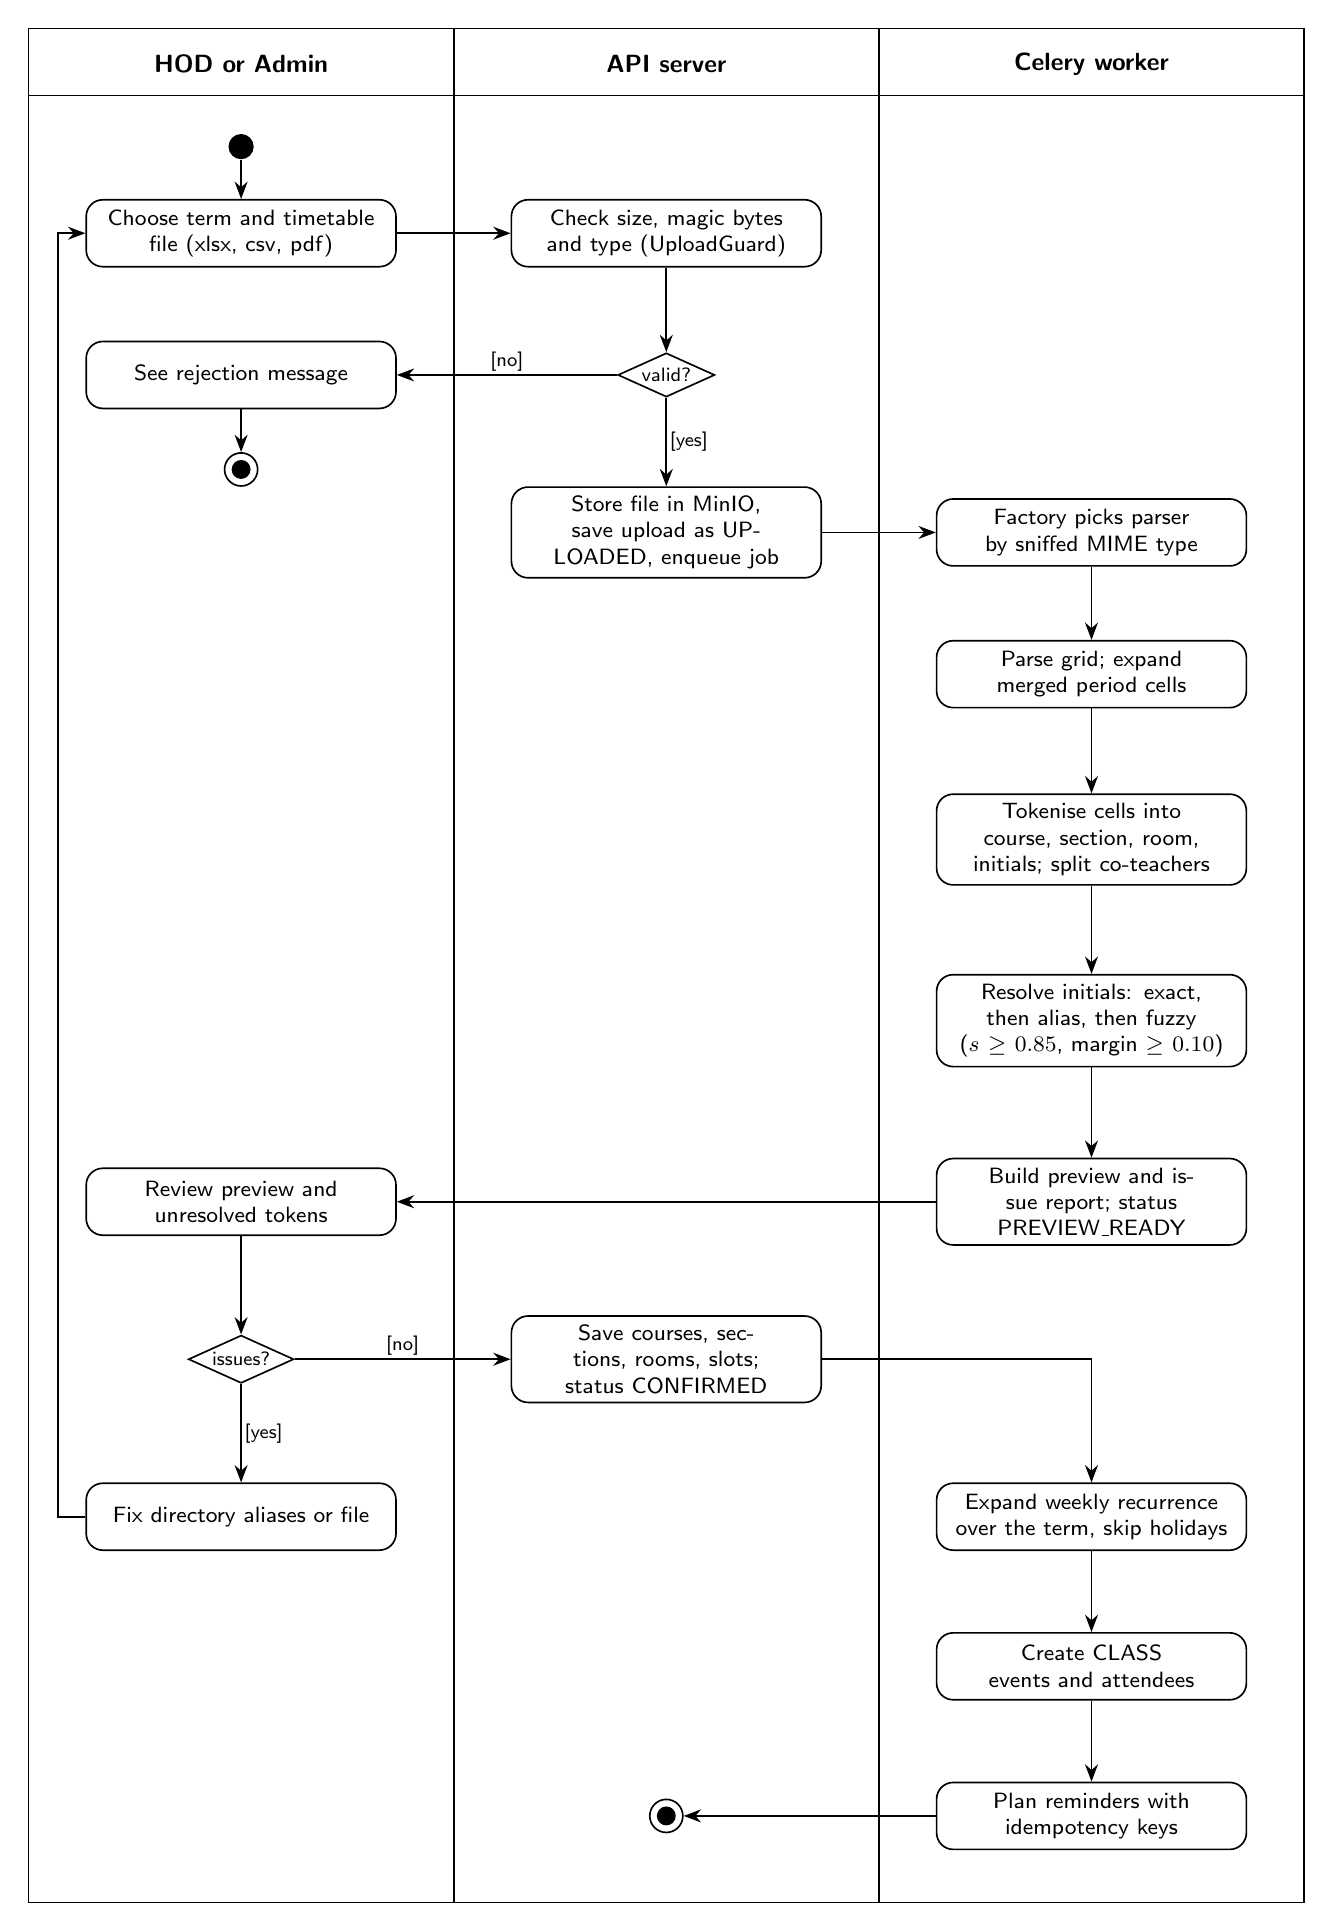
\begin{tikzpicture}[
    act/.style={rectangle, rounded corners=6pt, draw, semithick, fill=actfill, text width=3.7cm, align=center, font=\footnotesize, minimum height=0.85cm},
    dec/.style={diamond, draw, semithick, fill=decfill, aspect=2.2, font=\scriptsize, inner sep=1pt, align=center},
    fl/.style={semithick, -{Stealth[length=2.2mm]}},
    g/.style={font=\scriptsize, fill=white, inner sep=1pt}
  ]
  \def\lanew{5.4}
  \foreach \i/\name in {0/HOD or Admin, 1/API server, 2/Celery worker} {
    \draw[semithick] (\i*\lanew,0.6) rectangle ++(\lanew,-23.8);
    \node[font=\bfseries\small] at (\i*\lanew+\lanew/2,0.15) {\name};
  }
  \draw[semithick] (0,-0.25) -- (3*\lanew,-0.25);

  \node[initial] (s) at (2.7,-0.9) {};
  \node[act] (sel) at (2.7,-2.0) {Choose term and timetable file (xlsx, csv, pdf)};
  \node[act] (val) at (8.1,-2.0) {Check size, magic bytes and type (UploadGuard)};
  \node[dec] (ok) at (8.1,-3.8) {valid?};
  \node[act] (rej) at (2.7,-3.8) {See rejection message};
  \node[final] (e0) at (2.7,-5.0) {};
  \node[act] (store) at (8.1,-5.8) {Store file in MinIO, save upload as UPLOADED, enqueue job};

  \node[act] (fac) at (13.5,-5.8) {Factory picks parser by sniffed MIME type};
  \node[act] (parse) at (13.5,-7.6) {Parse grid; expand merged period cells};
  \node[act] (tok) at (13.5,-9.7) {Tokenise cells into course, section, room, initials; split co-teachers};
  \node[act] (res) at (13.5,-12.0) {Resolve initials: exact, then alias, then fuzzy ($s\ge0.85$, margin $\ge0.10$)};
  \node[act] (prev) at (13.5,-14.3) {Build preview and issue report; status PREVIEW\_READY};

  \node[act] (look) at (2.7,-14.3) {Review preview and unresolved tokens};
  \node[dec] (good) at (2.7,-16.3) {issues?};
  \node[act] (fix) at (2.7,-18.3) {Fix directory aliases or file};
  \node[act] (conf) at (8.1,-16.3) {Save courses, sections, rooms, slots; status CONFIRMED};

  \node[act] (exp) at (13.5,-18.3) {Expand weekly recurrence over the term, skip holidays};
  \node[act] (ev) at (13.5,-20.2) {Create CLASS events and attendees};
  \node[act] (rem) at (13.5,-22.1) {Plan reminders with idempotency keys};
  \node[final] (e1) at (8.1,-22.1) {};

  \draw[fl] (s) -- (sel);
  \draw[fl] (sel) -- (val);
  \draw[fl] (val) -- (ok);
  \draw[fl] (ok) -- node[g, above] {[no]} (rej);
  \draw[fl] (rej) -- (e0);
  \draw[fl] (ok) -- node[g, right] {[yes]} (store);
  \draw[fl] (store) -- (fac);
  \draw[fl] (fac) -- (parse);
  \draw[fl] (parse) -- (tok);
  \draw[fl] (tok) -- (res);
  \draw[fl] (res) -- (prev);
  \draw[fl] (prev) -- (look);
  \draw[fl] (look) -- (good);
  \draw[fl] (good) -- node[g, right] {[yes]} (fix);
  \draw[fl] (fix.west) -- ++(-0.35,0) |- (sel.west);
  \draw[fl] (good) -- node[g, above] {[no]} (conf);
  \draw[fl] (conf.east) -| (exp.north);
  \draw[fl] (exp) -- (ev);
  \draw[fl] (ev) -- (rem);
  \draw[fl] (rem) -- (e1);
\end{tikzpicture}
}
  \caption{Activity diagram: timetable ingestion and initials resolution}
  \label{fig:activity}
\end{figure}

\head{Explanation}
\begin{itemize}
  \item \textbf{Swimlanes:} the HOD, the API server and the Celery worker each perform their own actions.
  \item \textbf{First decision:} an invalid file is rejected before anything is stored.
  \item \textbf{Worker steps:} the factory chooses the parser; cells are split into course, section, room and initials; co-teacher cells are split; initials are resolved in three tiers.
  \item \textbf{Second decision and loop:} if the preview shows issues, the HOD fixes aliases or the file and uploads again; only a clean preview is confirmed.
  \item \textbf{After confirmation:} weekly recurrence is expanded over the term, holidays are skipped, CLASS events are created and reminders are planned.
\end{itemize}

\head{Activities Identified}
\needspace{7\baselineskip}
\begin{xltabular}{\textwidth}{|p{1cm}|Y|p{2.6cm}|p{3cm}|}
\caption{Activities in timetable ingestion}\\
\hline
\textbf{No.} & \textbf{Activity} & \textbf{Swimlane} & \textbf{Type} \\ \hline
1 & Choose term and timetable file & HOD & Action \\ \hline
2 & Check size, file type and content & API server & Action + decision \\ \hline
3 & Store file and enqueue the job & API server & Action \\ \hline
4 & Pick parser and parse the grid & Worker & Action \\ \hline
5 & Tokenise cells and split co-teachers & Worker & Action \\ \hline
6 & Resolve initials (exact, alias, fuzzy) & Worker & Action \\ \hline
7 & Build preview and issue report & Worker & Action \\ \hline
8 & Review preview; fix issues if any & HOD & Decision (loop to 1) \\ \hline
9 & Save courses, sections, rooms, slots & API server & Action \\ \hline
10 & Expand recurrence, create events, plan reminders & Worker & Action \\ \hline
\end{xltabular}

\head{Conclusion}
The activity diagram models the complete ingestion workflow, including the validation stop, the fix-and-retry loop and the division of work between the HOD, the API and the background worker.

\subsection{Package Diagram}

\theory{Theory}
A package diagram groups model elements or code into packages and shows the dependencies between them. A package is drawn as a folder (\sympkg); a dependency is a dashed arrow, often labelled \guill{import} or \guill{use}. It is used to check that the layering of a system is respected.

\begin{figure}[!htbp]
  \centering
  \resizebox{0.95\textwidth}{!}{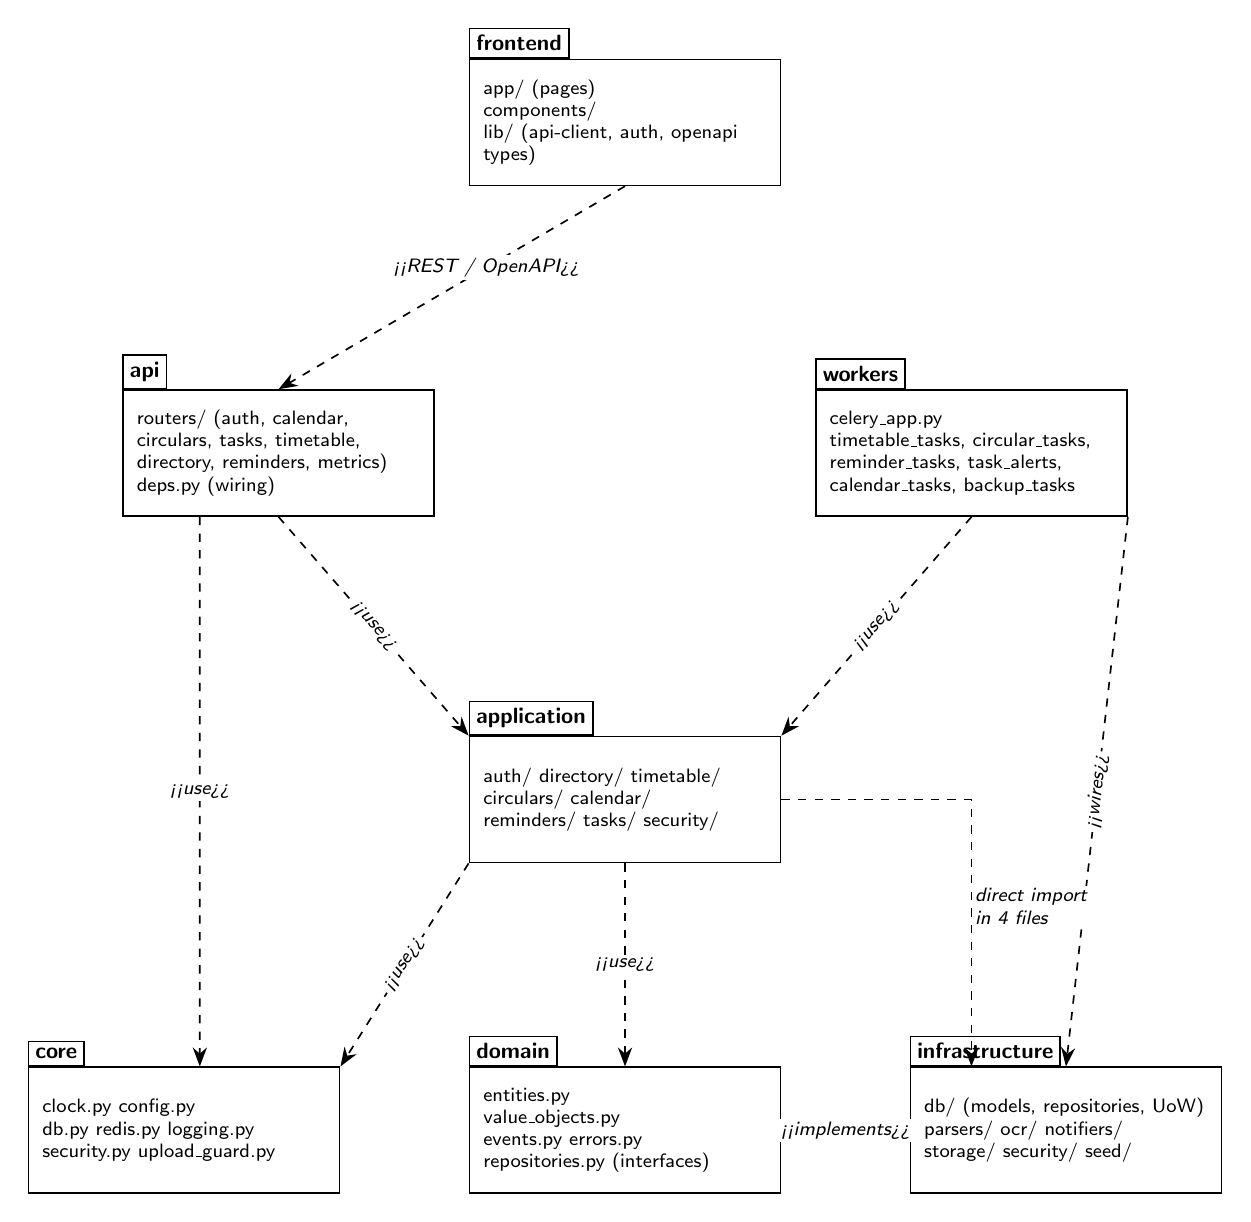
\begin{tikzpicture}[
    pkg/.style={rectangle, draw, semithick, fill=#1, align=left, font=\scriptsize\sffamily, inner sep=5pt, text width=3.6cm, minimum height=1.6cm},
    pkg/.default=white,
    tab/.style={draw, semithick, fill=white, font=\footnotesize\bfseries, inner sep=2.5pt, anchor=south west},
    imp/.style={semithick, dashed, -{Stealth[length=2.4mm]}},
    bad/.style={semithick, dashed, black, -{Stealth[length=2.4mm]}},
    lbl/.style={font=\scriptsize\itshape, fill=white, inner sep=1pt}
  ]
  \newcommand{\pkgnode}[5]{\node[pkg=#4] (#1) at (#2) {#5}; \node[tab] at (#1.north west) {#3};}

  \pkgnode{fe}{7.0,4.2}{frontend}{white}{app/ (pages)\\components/\\lib/ (api-client, auth, openapi types)}

  \pkgnode{api}{2.6,0}{api}{white}{routers/ (auth, calendar,\\ circulars, tasks, timetable,\\ directory, reminders, metrics)\\deps.py (wiring)}
  \pkgnode{workers}{11.4,0}{workers}{white}{celery\_app.py\\timetable\_tasks, circular\_tasks,\\reminder\_tasks, task\_alerts,\\calendar\_tasks, backup\_tasks}

  \pkgnode{app}{7.0,-4.4}{application}{white}{auth/ directory/ timetable/\\circulars/ calendar/\\reminders/ tasks/ security/}

  \pkgnode{infra}{12.6,-8.6}{infrastructure}{white}{db/ (models, repositories, UoW)\\parsers/ ocr/ notifiers/\\storage/ security/ seed/}

  \pkgnode{dom}{7.0,-8.6}{domain}{white}{entities.py\\value\_objects.py\\events.py  errors.py\\repositories.py (interfaces)}

  \pkgnode{core}{1.4,-8.6}{core}{white}{clock.py  config.py\\db.py  redis.py  logging.py\\security.py  upload\_guard.py}

  \draw[imp] (fe.south) -- node[lbl, pos=0.4] {\guill{REST / OpenAPI}} (api.north);
  \draw[imp] (api.south) -- node[lbl, sloped] {\guill{use}} (app.north west);
  \draw[imp] (workers.south) -- node[lbl, sloped] {\guill{use}} (app.north east);
  \draw[imp] (app) -- node[lbl] {\guill{use}} (dom);
  \draw[imp] (infra) -- node[lbl] {\guill{implements}} (dom);
  \draw[imp] (workers.south east) -- node[lbl, sloped] {\guill{wires}} (infra.north);
  \draw[imp] (app.south west) -- node[lbl, sloped] {\guill{use}} (core.north east);
  \draw[imp] (api.south) ++(-1.0,0) -- node[lbl] {\guill{use}} ([xshift=0.2cm]core.north);
  \draw[bad] (app.east) -| node[lbl, pos=0.7, right, text=black, align=left] {direct import\\in 4 files} ([xshift=-1.2cm]infra.north);
\end{tikzpicture}
}
  \caption{Package diagram with import dependencies}
  \label{fig:package}
\end{figure}

\head{Explanation}
\begin{itemize}
  \item The \textbf{frontend} calls the backend only through the REST API described by an OpenAPI contract.
  \item \textbf{api} and \textbf{workers} call \textbf{application}; \textbf{workers} (and \texttt{api/deps.py}) wire the concrete adapters from \textbf{infrastructure}.
  \item \textbf{infrastructure} implements the repository interfaces declared in \textbf{domain}.
  \item \textbf{domain} imports nothing outside itself; we checked this by scanning every import in the backend.
  \item The arrow labelled \emph{direct import} marks four application files that import infrastructure classes (OCR engine and extractor, parser factory and initials resolver, notifier base class, MinIO storage). Moving these behind domain interfaces would complete the layering.
\end{itemize}

\head{Conclusion}
The package diagram confirms that the business core (\texttt{domain}) is independent of frameworks and shows the one place where the layering is not yet complete.

\subsection{Component Diagram}

\theory{Theory}
A component diagram shows the replaceable parts of a running system and the interfaces through which they connect. A component (\symcompnt) provides interfaces, drawn as a ball (\symball), and requires interfaces from other components.

\begin{figure}[!htbp]
  \centering
  \resizebox{\textwidth}{!}{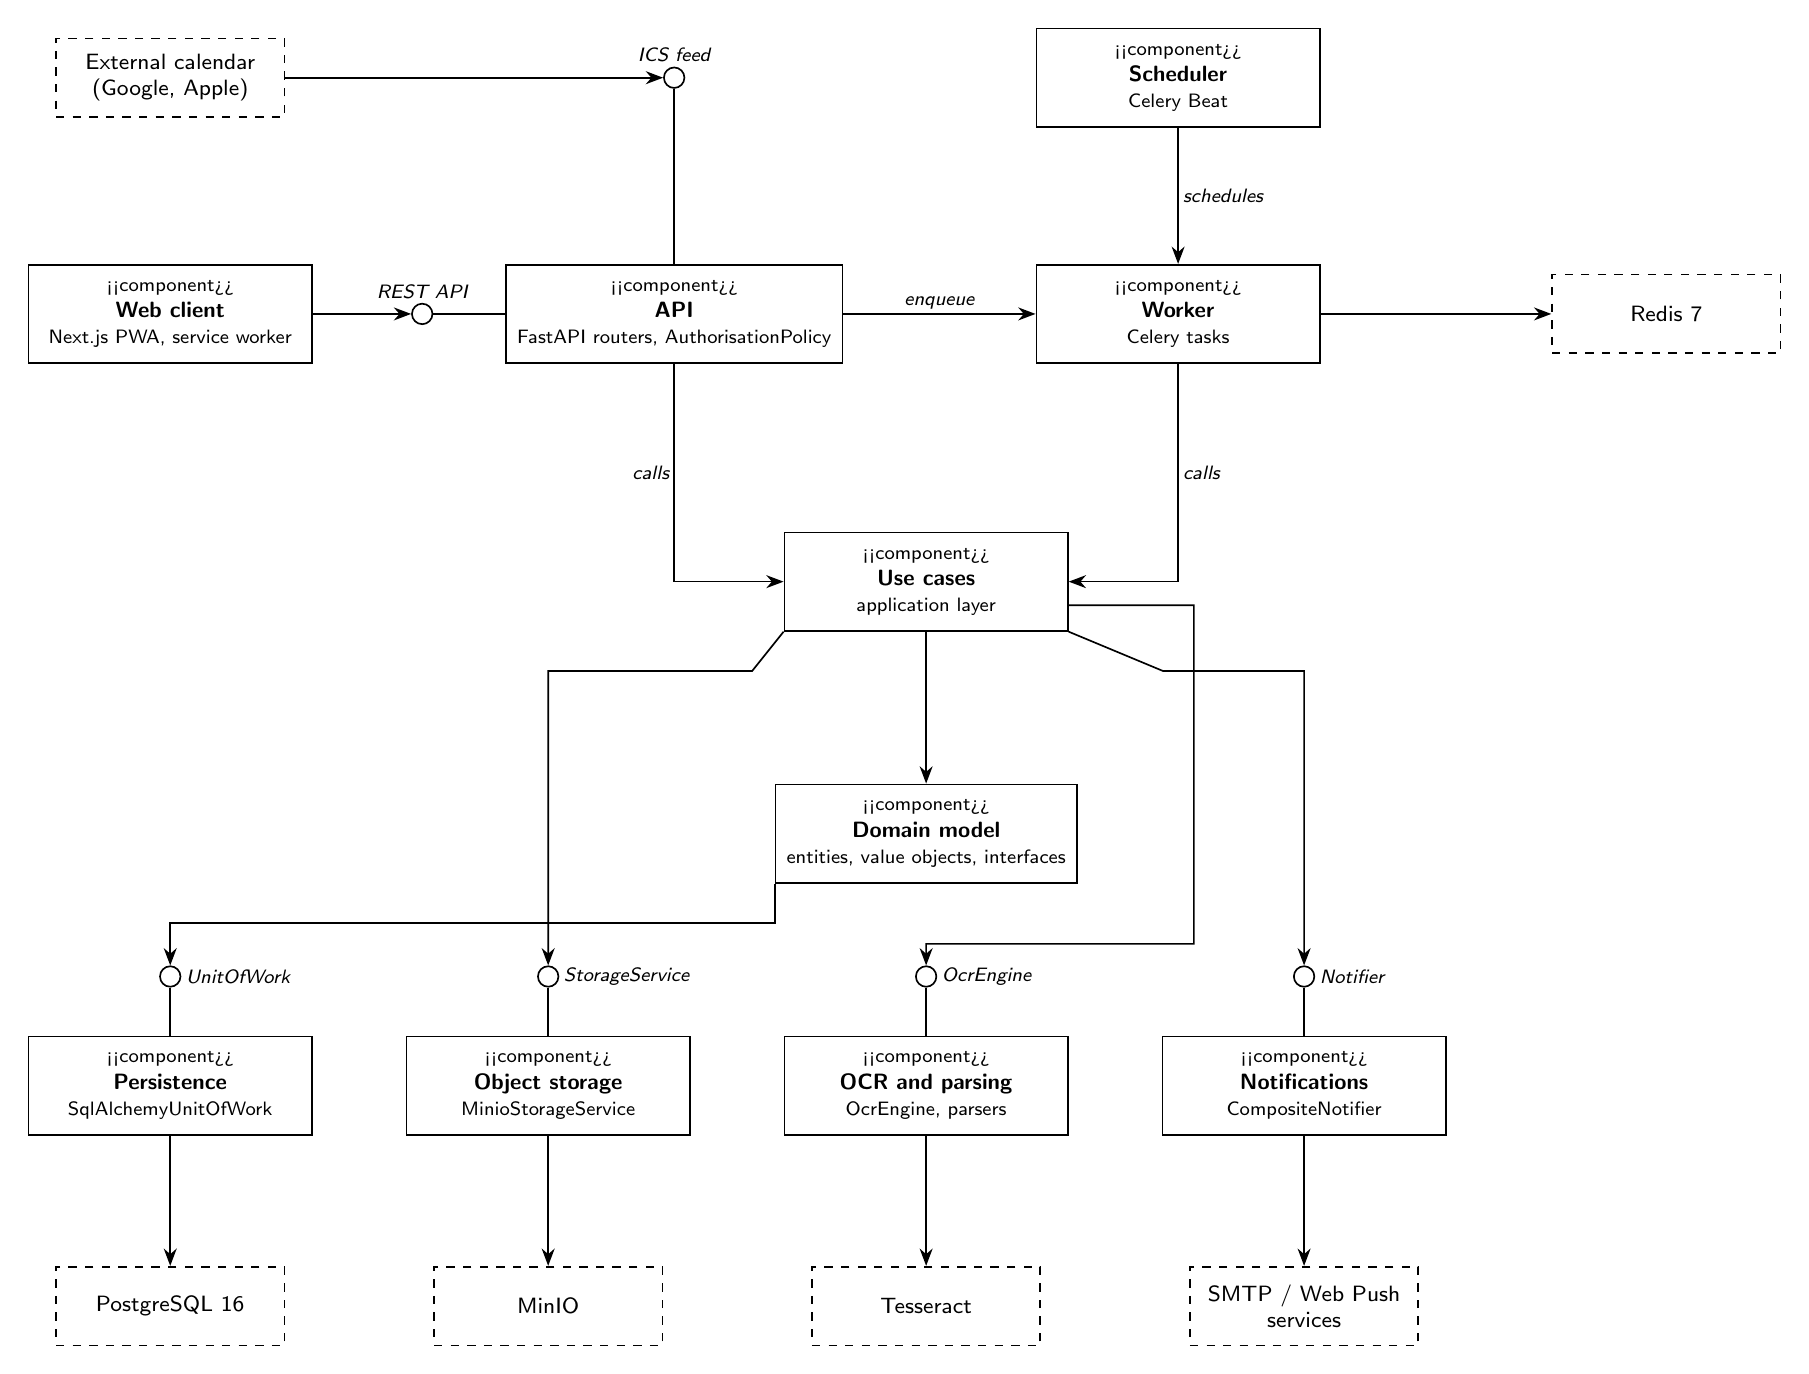
\begin{tikzpicture}[
    comp/.style={rectangle, draw, semithick, fill=#1, align=center, font=\footnotesize, minimum width=3.6cm, minimum height=1.25cm, inner sep=4pt},
    comp/.default=white,
    ext/.style={rectangle, draw, semithick, dashed, fill=white, align=center, font=\footnotesize, minimum width=2.9cm, minimum height=1.0cm},
    con/.style={semithick, -{Stealth[length=2.2mm]}},
    ball/.style={circle, draw, semithick, fill=white, minimum size=2.6mm, inner sep=0pt},
    ilbl/.style={font=\scriptsize\itshape, inner sep=1.5pt, align=center}
  ]
  \newcommand{\cname}[2]{{\scriptsize\guill{component}}\\\textbf{#1}\\{\scriptsize #2}}

  \node[comp=white] (fe) at (0,0) {\cname{Web client}{Next.js PWA, service worker}};
  \node[comp=white] (api) at (6.4,0) {\cname{API}{FastAPI routers, AuthorisationPolicy}};
  \node[comp=white] (worker) at (12.8,0) {\cname{Worker}{Celery tasks}};
  \node[comp=white] (beat) at (12.8,3.0) {\cname{Scheduler}{Celery Beat}};
  \node[comp=white] (uc) at (9.6,-3.4) {\cname{Use cases}{application layer}};
  \node[comp=white] (dom) at (9.6,-6.6) {\cname{Domain model}{entities, value objects, interfaces}};

  \node[comp=white] (persist) at (0,-9.8) {\cname{Persistence}{SqlAlchemyUnitOfWork}};
  \node[comp=white] (store) at (4.8,-9.8) {\cname{Object storage}{MinioStorageService}};
  \node[comp=white] (ocr) at (9.6,-9.8) {\cname{OCR and parsing}{OcrEngine, parsers}};
  \node[comp=white] (notify) at (14.4,-9.8) {\cname{Notifications}{CompositeNotifier}};

  \node[ext] (pg) at (0,-12.6) {PostgreSQL 16};
  \node[ext] (minio) at (4.8,-12.6) {MinIO};
  \node[ext] (tess) at (9.6,-12.6) {Tesseract};
  \node[ext] (smtp) at (14.4,-12.6) {SMTP / Web Push\\services};
  \node[ext] (redis) at (19.0,0) {Redis 7};
  \node[ext] (cal) at (0,3.0) {External calendar\\(Google, Apple)};

  \node[ball] (restball) at (3.2,0) {};
  \node[ilbl, above] at (restball.north) {REST API};
  \draw[semithick] (api.west) -- (restball);
  \draw[con] (fe.east) -- (restball.west);
  \node[ball] (icsball) at (6.4,3.0) {};
  \node[ilbl, above] at (icsball.north) {ICS feed};
  \draw[semithick] (api.north) -- (icsball);
  \draw[con] (cal.east) -- (icsball.west);

  \draw[con] (api.south) |- node[ilbl, pos=0.25, left] {calls} (uc.west);
  \draw[con] (worker.south) |- node[ilbl, pos=0.25, right] {calls} (uc.east);
  \draw[con] (beat) -- node[ilbl, right] {schedules} (worker);
  \draw[con] (api.east) -- node[ilbl, above] {enqueue} (worker.west);
  \draw[con] (worker.east) -- (redis.west);
  \draw[con] (uc) -- (dom);

  \foreach \c/\i in {persist/UnitOfWork, store/StorageService, ocr/OcrEngine, notify/Notifier} {
    \node[ball] (\c b) at ($(\c.north)+(0,0.75)$) {};
    \node[ilbl, right] at (\c b.east) {\i};
    \draw[semithick] (\c.north) -- (\c b);
  }
  \draw[con] (dom.south west) -- ++(0,-0.5) -| (persistb.north);
  \draw[con] (uc.south west) -- ++(-0.4,-0.5) -| (storeb.north);
  \draw[con] (uc.south east) -- ++(1.2,-0.5) -| (notifyb.north);
  \draw[con] ([yshift=-3mm]uc.east) -- (13.0,-3.7) -- (13.0,-8.0) -| (ocrb.north);

  \draw[con] (persist) -- (pg);
  \draw[con] (store) -- (minio);
  \draw[con] (ocr) -- (tess);
  \draw[con] (notify) -- (smtp);
\end{tikzpicture}
}
  \caption{Component diagram with provided interfaces}
  \label{fig:component}
\end{figure}

\head{Components Identified}
{\small
\needspace{7\baselineskip}
\begin{xltabular}{\textwidth}{|p{3.2cm}|Y|p{4.2cm}|}
\caption{Components and interfaces}\\
\hline
\textbf{Component} & \textbf{Responsibility} & \textbf{Interface} \\ \hline
Web client & Screens for all roles; offline cache and push handler & requires REST API \\ \hline
API & Routers, validation, role checks & provides REST API, ICS feed \\ \hline
Worker / Scheduler & Background jobs and periodic schedule & uses Redis queue \\ \hline
Use cases & One class per user goal & requires UnitOfWork, StorageService, OcrEngine, Notifier \\ \hline
Domain model & Entities, value objects, interfaces & declares repository interfaces \\ \hline
Persistence & SQLAlchemy repositories and unit of work & provides UnitOfWork \\ \hline
Object storage & File upload and download in MinIO & provides StorageService \\ \hline
OCR and parsing & Tesseract OCR, timetable parsers & provides OcrEngine \\ \hline
Notifications & E-mail and web push & provides Notifier \\ \hline
\end{xltabular}}

\head{Conclusion}
The component diagram shows that the API and the worker share the same use-case component, and that every external service is reached through one adapter, so it can be replaced without changing the use cases. \texttt{UnitOfWork} and \texttt{Notifier} are abstract types in the code; \texttt{OcrEngine} and \texttt{StorageService} are concrete classes today.

\subsection{Deployment Diagram}

\theory{Theory}
A deployment diagram shows the physical nodes (devices and execution environments, drawn as 3-D boxes \symnode), the artifacts deployed on them, and the communication paths between nodes.

\begin{figure}[!htbp]
  \centering
  \resizebox{\textwidth}{!}{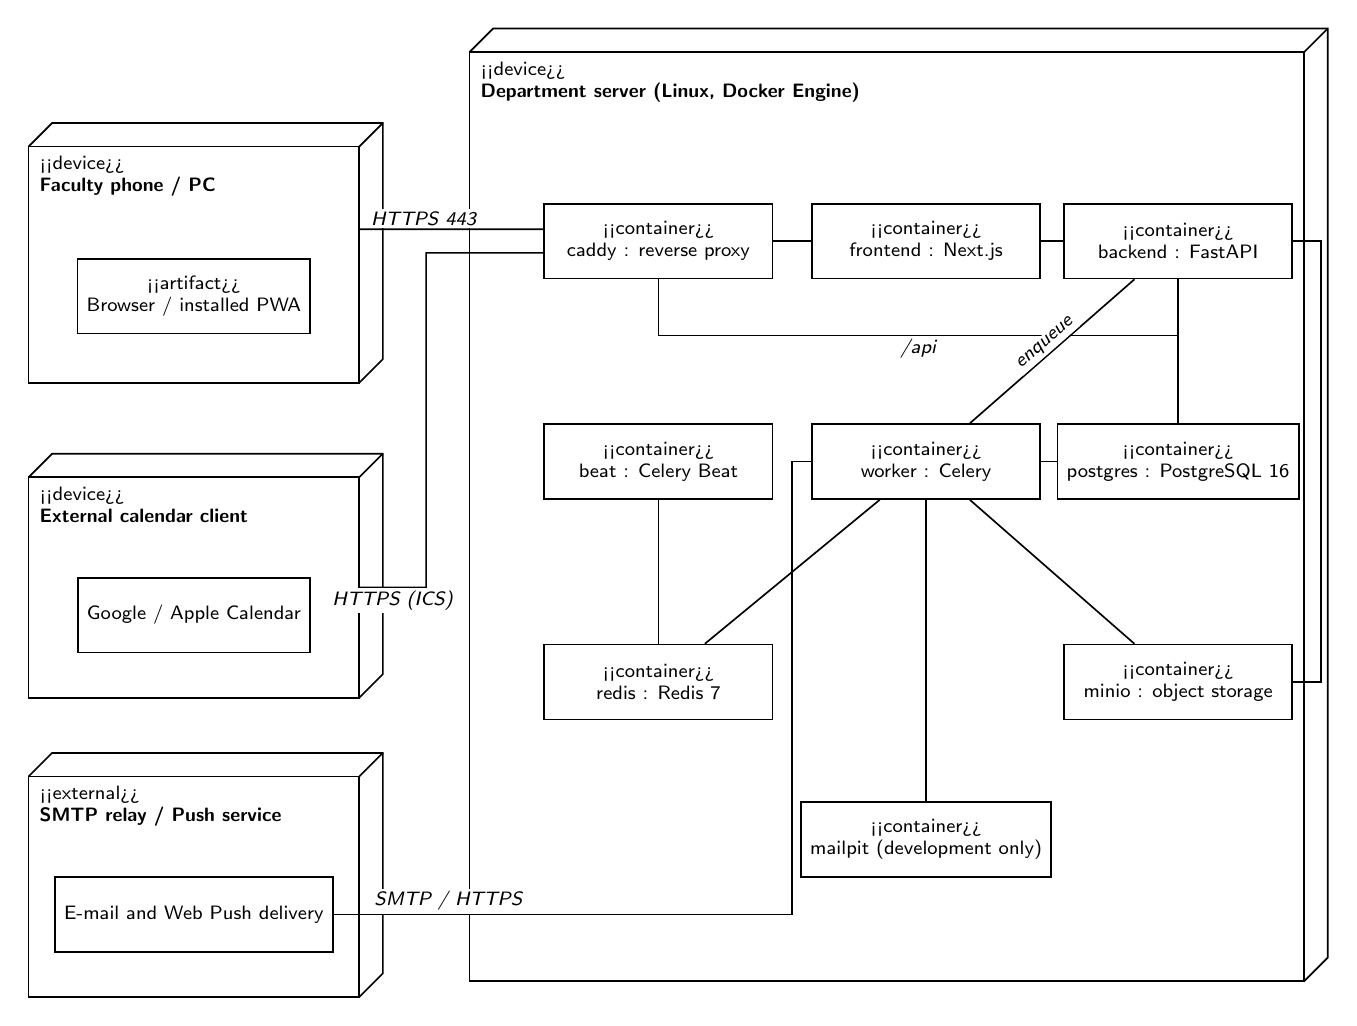
\begin{tikzpicture}[
    art/.style={rectangle, draw, semithick, fill=white, font=\scriptsize, align=center, minimum width=2.9cm, minimum height=0.95cm},
    path/.style={semithick},
    l/.style={font=\scriptsize\itshape, fill=white, inner sep=1pt, align=center}
  ]
  \newcommand{\umlnode}[5]{%
    \draw[semithick, fill=white] (#1) rectangle ++(#2,-#3);
    \draw[semithick] (#1) -- ++(0.3,0.3) -- ++(#2,0) -- ++(0,-#3) -- ++(-0.3,-0.3);
    \draw[semithick] ($(#1)+(#2,0)$) -- ++(0.3,0.3);
    \node[anchor=north west, font=\scriptsize, align=left, fill=white, inner sep=1pt] at ($(#1)+(0.1,-0.08)$) {\guill{#4}\\\textbf{#5}};}

  \umlnode{0,0}{4.2}{3.0}{device}{Faculty phone / PC}
  \node[art] at (2.1,-1.9) {\guill{artifact}\\Browser / installed PWA};

  \umlnode{0,-4.2}{4.2}{2.8}{device}{External calendar client}
  \node[art] at (2.1,-5.95) {Google / Apple Calendar};

  \umlnode{5.6,1.2}{10.6}{11.8}{device}{Department server (Linux, Docker Engine)}
  \node[art] (caddy) at (8.0,-1.2) {\guill{container}\\caddy : reverse proxy};
  \node[art] (fe) at (11.4,-1.2) {\guill{container}\\frontend : Next.js};
  \node[art] (be) at (14.6,-1.2) {\guill{container}\\backend : FastAPI};
  \node[art] (wk) at (11.4,-4.0) {\guill{container}\\worker : Celery};
  \node[art] (bt) at (8.0,-4.0) {\guill{container}\\beat : Celery Beat};
  \node[art] (pg) at (14.6,-4.0) {\guill{container}\\postgres : PostgreSQL 16};
  \node[art] (rd) at (8.0,-6.8) {\guill{container}\\redis : Redis 7};
  \node[art] (mn) at (14.6,-6.8) {\guill{container}\\minio : object storage};
  \node[art] (mp) at (11.4,-8.8) {\guill{container}\\mailpit (development only)};

  \umlnode{0,-8.0}{4.2}{2.8}{external}{SMTP relay / Push service}
  \node[art] (ext) at (2.1,-9.75) {E-mail and Web Push delivery};

  \draw[path] (4.2,-1.05) -- node[l, above, pos=0.35] {HTTPS 443} ([yshift=1.5mm]caddy.west);
  \draw[path] (4.2,-5.6) -- node[l, below, pos=0.5] {HTTPS (ICS)} (5.05,-5.6) -- (5.05,-1.35) -- ([yshift=-1.5mm]caddy.west);
  \draw[path] (caddy) -- (fe);
  \draw[path] (fe) -- (be);
  \draw[path] (caddy.south) -- (8.0,-2.4) -| node[l, pos=0.25, below] {/api} (be.south);
  \draw[path] (be) -- (pg);
  \draw[path] (be.east) -- ++(0.35,0) |- (mn.east);
  \draw[path] (wk) -- (pg);
  \draw[path] (wk) -- (rd);
  \draw[path] (wk) -- (mn);
  \draw[path] (bt) -- (rd);
  \draw[path] (be) -- node[l, sloped, above] {enqueue} (wk);
  \draw[path] (wk) -- (mp);
  \draw[path] (ext.east) -- node[l, above, pos=0.25] {SMTP / HTTPS} (9.7,-9.75) -- (9.7,-4.0) -- (wk.west);
\end{tikzpicture}
}
  \caption{Deployment diagram (production on a department server)}
  \label{fig:deployment}
\end{figure}

\head{Explanation}
\begin{itemize}
  \item All server parts run as containers on one machine under Docker Compose; application containers run as a non-root user.
  \item Browsers, the installed phone app and external calendar apps reach only the Caddy container over HTTPS. Caddy sends \texttt{/api} requests to the backend and all other requests to the frontend.
  \item The worker and the scheduler share PostgreSQL, Redis and MinIO with the backend; the worker delivers e-mail and web push to outside services.
  \item In \emph{college-LAN mode} Caddy uses an internal certificate, so the system can run inside the campus network without a public domain.
\end{itemize}

\head{Conclusion}
The deployment diagram shows that the complete system fits on one department server and needs no paid service.

\subsection{Entity--Relationship Diagram}
The ER diagram in Figure~\ref{fig:er} is generated by a script directly from the database model definitions, so its 20 tables, columns and keys match the database exactly. All timestamps are stored as \texttt{timestamptz} in UTC. Unique keys enforce business rules in the database itself, for example one \texttt{idempotency\_key} per reminder and one \texttt{ics\_token} per faculty member. Because the schema is wide, the diagram is rotated on the page.

\begin{figure}[H]
  \centering
  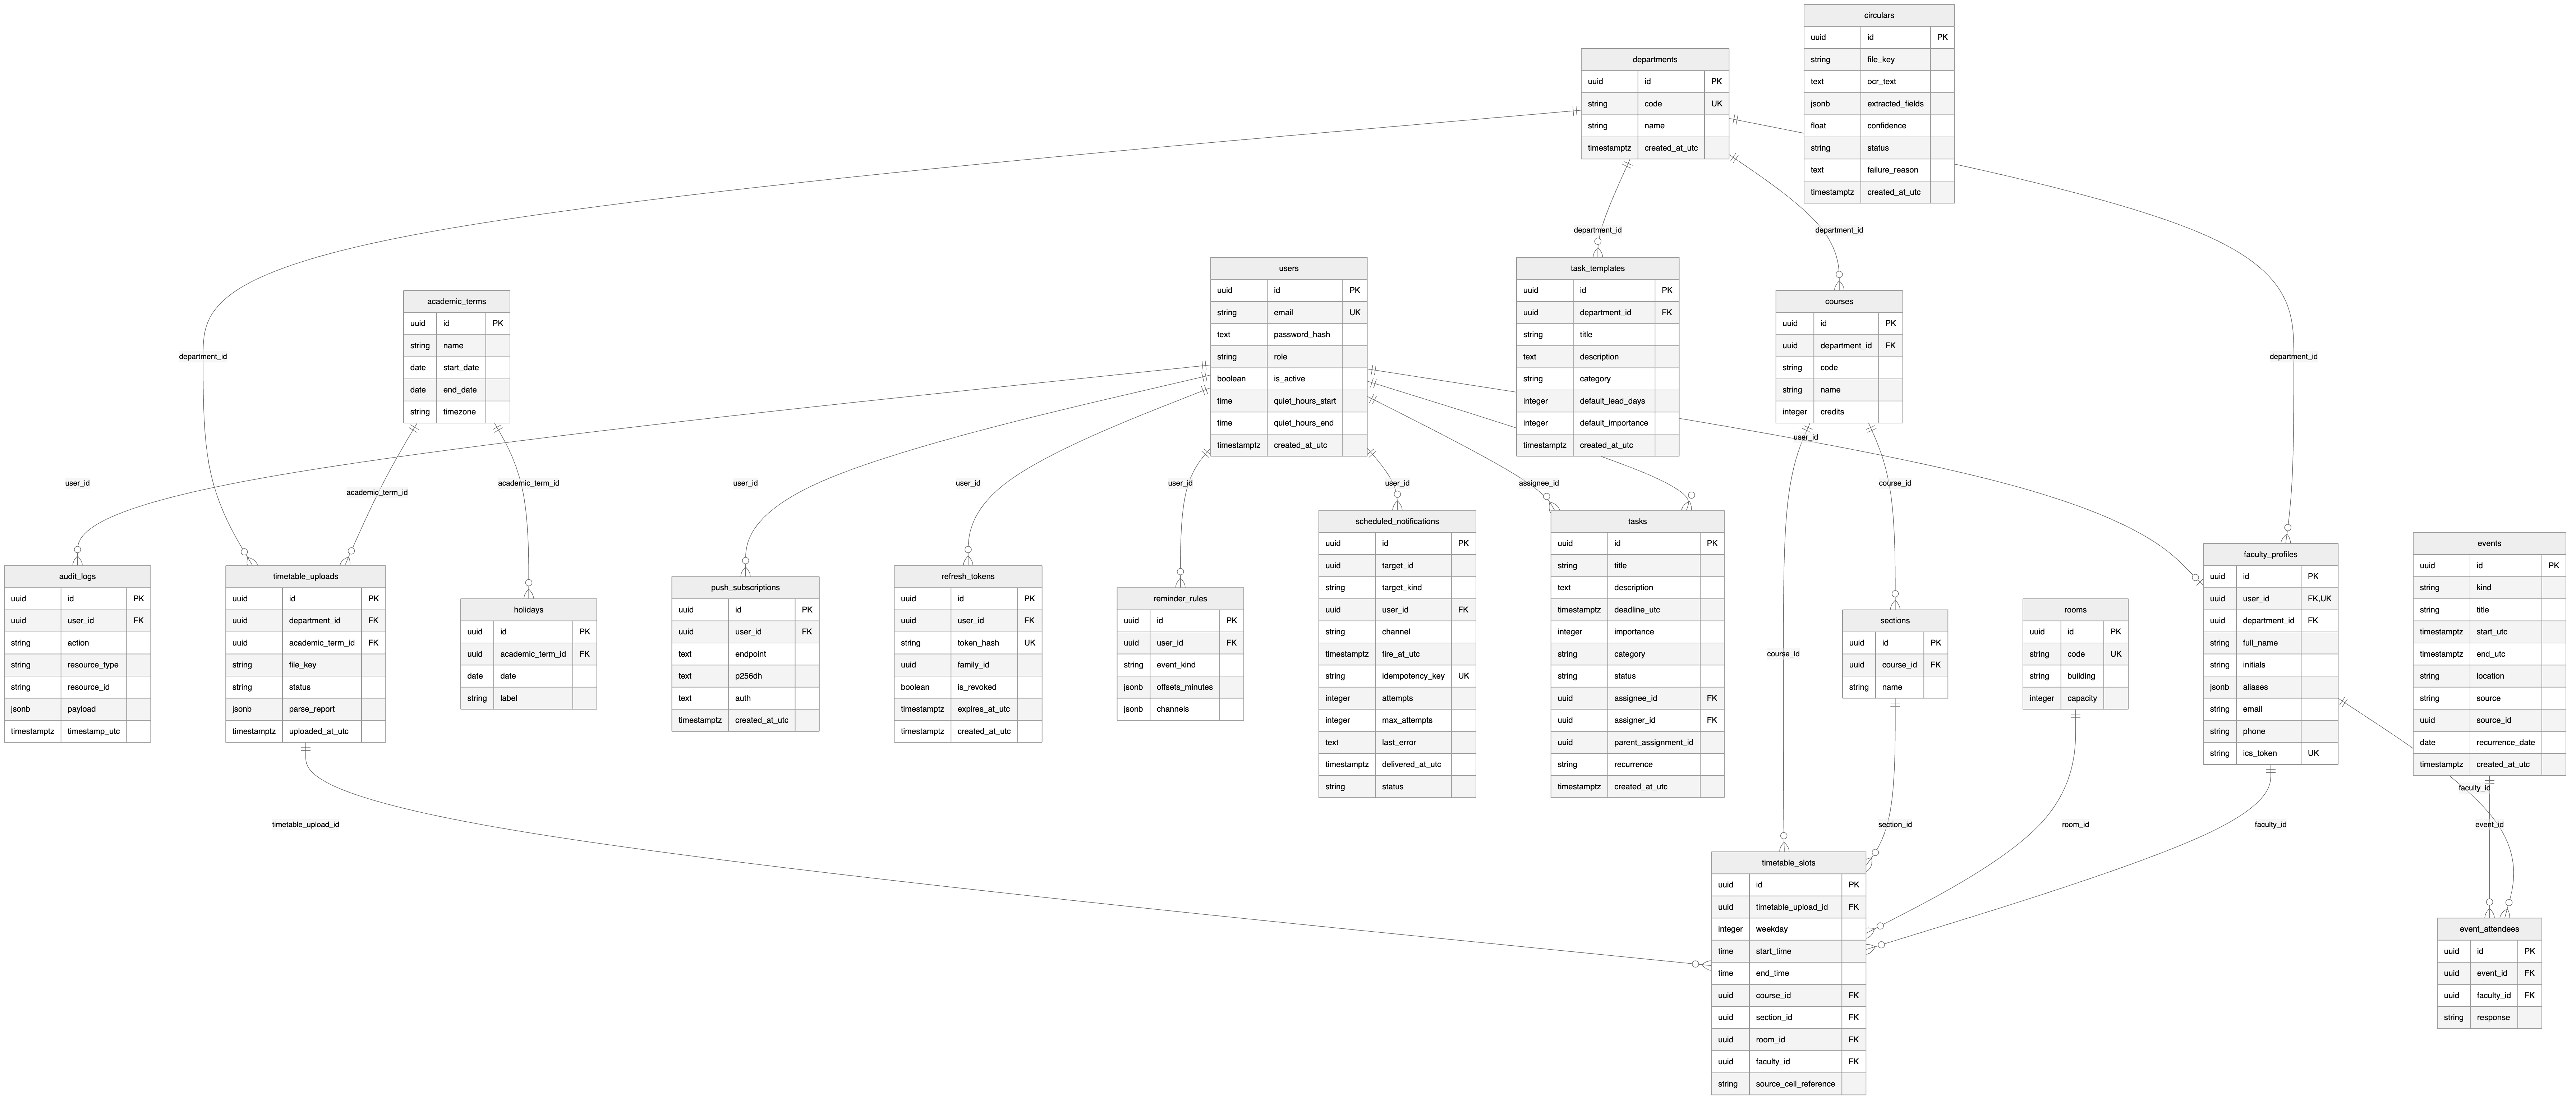
\includegraphics[angle=90, height=0.74\textheight, width=\textwidth, keepaspectratio]{figures/er-generated.png}
  \caption{Entity--relationship diagram of the PostgreSQL schema}
  \label{fig:er}
\end{figure}

\newsection{Object-Oriented Analysis, Design \& Architecture}{sec:ooad}

\subsection{Object-Oriented Analysis}
Object-oriented analysis finds the classes of the problem domain before any design decision is made. We used the noun analysis method [2]: mark the nouns of the problem statement, classify them, filter out the ones that are not classes, and add classes that domain knowledge requires.

\head{Step 1: Potential Objects (Nouns and Noun Phrases)}
From the problem statement in Section~\ref{sec:objectives}: department, system, calendar, faculty member, HOD, timetable, timetable file, cell, initials, teacher, class, term, holiday, photo, meeting circular, date, time, venue, name, meeting, details, reminder, e-mail, phone notification, quiet hours, documentation task, group, deadline, work, alert.

\head{Step 2: Classification}
\needspace{7\baselineskip}
\begin{xltabular}{\textwidth}{|p{3.2cm}|Y|}
\caption{Classification of candidate objects}\\
\hline
\textbf{Category} & \textbf{Candidates} \\ \hline
People and roles & faculty member, teacher, HOD, group \\ \hline
Organisations & department \\ \hline
Things and documents & timetable file, cell, photo, meeting circular, e-mail, phone notification \\ \hline
Concepts & calendar, initials, quiet hours, details, term \\ \hline
Events & class, meeting, holiday, deadline, reminder, alert, documentation task \\ \hline
Attributes & date, time, venue, name \\ \hline
\end{xltabular}

\head{Step 3: Filtering}
\needspace{7\baselineskip}
\begin{xltabular}{\textwidth}{|p{3.6cm}|p{3.4cm}|Y|}
\caption{Filtering of candidates}\\
\hline
\textbf{Candidate} & \textbf{Decision} & \textbf{Reason} \\ \hline
system & Removed & It is the system itself, not a domain object. \\ \hline
teacher, faculty member & Merged $\rightarrow$ FacultyProfile & Same person; profile holds initials and aliases. \\ \hline
HOD, Admin & Role of User & They differ only in permissions (\texttt{Role} value). \\ \hline
class, meeting, deadline & Merged $\rightarrow$ Event & One interval type with a \texttt{kind}; clash checks and reminders treat them alike. \\ \hline
reminder, alert & Merged $\rightarrow$ ScheduledNotification & One planned send with its own life cycle. \\ \hline
date, time, venue, name & Attributes & Properties of Event or FacultyProfile. \\ \hline
initials, quiet hours & Value objects & Defined only by their value; must validate themselves. \\ \hline
cell & Merged $\rightarrow$ TimetableSlot & A parsed cell is one weekly slot. \\ \hline
e-mail, phone notification & Channel value & Delivery channel of a notification. \\ \hline
calendar, details, group & Removed & A view over events, too vague, or a set of profiles. \\ \hline
\end{xltabular}

\head{Step 4: Classes Added from Domain Knowledge}
\begin{itemize}
  \item \textbf{User} -- the log-in account, separate from the faculty profile (an Admin may have no profile).
  \item \textbf{TimetableUpload} -- one uploaded file with its parse report and status.
  \item \textbf{EventAttendee} -- links a faculty member to an event with a response.
  \item \textbf{ReminderRule} -- a user's lead times and channels for each kind of event.
  \item \textbf{AcademicTerm} -- the term dates and time zone that bound class generation.
\end{itemize}

\head{Step 5: Final Domain Classes}
Department, User, FacultyProfile, AcademicTerm, Holiday, Course, Section, Room, TimetableUpload, TimetableSlot, Event, EventAttendee, Circular, ScheduledNotification, ReminderRule, PushSubscription, Task, TaskTemplate, AuditLog, RefreshToken; value objects Initials, TimeSlot and QuietHours.

\subsection{Object-Oriented Design}

\head{Layered (Clean) Architecture}
The backend is divided into four layers [5]. Dependencies point inwards, towards the domain.

\begin{figure}[!htbp]
\centering
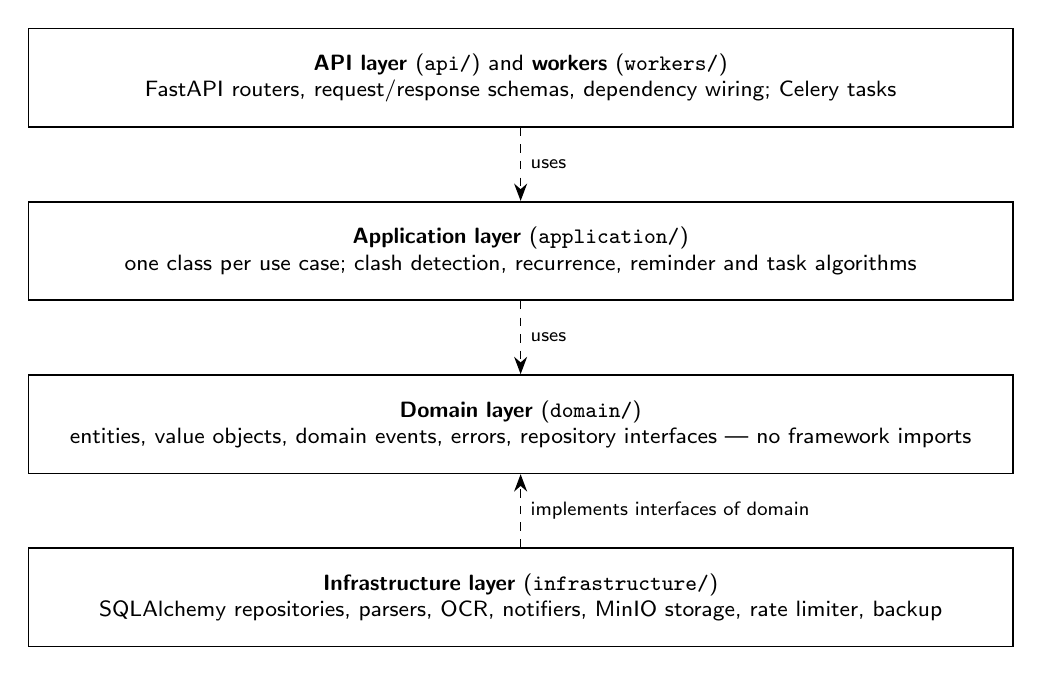
\begin{tikzpicture}[
  lay/.style={rectangle, draw, semithick, align=center, font=\footnotesize, minimum width=12.5cm, minimum height=1.25cm, text width=12cm},
  ar/.style={semithick, dashed, -{Stealth[length=2.2mm]}}]
  \node[lay] (api) at (0,0) {\textbf{API layer} (\texttt{api/}) and \textbf{workers} (\texttt{workers/})\\FastAPI routers, request/response schemas, dependency wiring; Celery tasks};
  \node[lay] (app) at (0,-2.2) {\textbf{Application layer} (\texttt{application/})\\one class per use case; clash detection, recurrence, reminder and task algorithms};
  \node[lay] (dom) at (0,-4.4) {\textbf{Domain layer} (\texttt{domain/})\\entities, value objects, domain events, errors, repository interfaces --- no framework imports};
  \node[lay] (inf) at (0,-6.6) {\textbf{Infrastructure layer} (\texttt{infrastructure/})\\SQLAlchemy repositories, parsers, OCR, notifiers, MinIO storage, rate limiter, backup};
  \draw[ar] (api) -- node[right, font=\scriptsize] {uses} (app);
  \draw[ar] (app) -- node[right, font=\scriptsize] {uses} (dom);
  \draw[ar] (inf) -- node[right, font=\scriptsize] {implements interfaces of domain} (dom);
\end{tikzpicture}
\caption{Layered architecture of the backend}
\label{fig:layers}
\end{figure}

Use cases receive their collaborators through their constructors (dependency injection). The same \texttt{ProcessCircularUseCase} therefore runs in a worker in production and in a test with a test database, and the same \texttt{ReminderDispatcher} runs with \texttt{SystemClock} in production and with \texttt{FrozenClock} in tests. As shown in the package diagram, four application files still import infrastructure classes directly; the domain layer has no outward imports at all.

\head{Design Principles Applied}
\needspace{7\baselineskip}
\begin{xltabular}{\textwidth}{|p{3.6cm}|Y|}
\caption{Design principles}\\
\hline
\textbf{Principle} & \textbf{How FacultyDesk applies it} \\ \hline
Single responsibility & Each use-case class serves one goal; \texttt{InitialsResolver} only resolves initials; \texttt{CircularExtractor} only extracts fields. \\ \hline
Open--closed & A new timetable format needs a new \texttt{TimetableParser} subclass and one line in the factory; a new channel (such as SMS) needs a new \texttt{Notifier}. \\ \hline
Liskov substitution & Any \texttt{Notifier} can be given to the dispatcher; tests substitute frozen-time and test-database objects. \\ \hline
Interface segregation & Eighteen small repository interfaces, one per aggregate, instead of one large data-access class. \\ \hline
Dependency inversion & Use cases depend on \texttt{UnitOfWork}, \texttt{Notifier} and \texttt{Clock} abstractions, not on SQLAlchemy or SMTP. \\ \hline
Information expert (GRASP) & \texttt{QuietHours} decides whether a time is quiet; \texttt{Circular} decides which status change is legal; \texttt{Task} validates its own importance and deadline. \\ \hline
\end{xltabular}

\head{Design Patterns}
The patterns follow the catalogues of Gamma \emph{et al.} [3] and Fowler [4]. Figures~\ref{fig:classpatterns} and \ref{fig:classpatternsb} show the classes involved.

{\small
\needspace{7\baselineskip}
\begin{xltabular}{\textwidth}{|p{2.6cm}|p{4.6cm}|Y|}
\caption{Design patterns used}\\
\hline
\textbf{Pattern} & \textbf{Classes} & \textbf{Problem it solves} \\ \hline
Repository & EventRepository, TaskRepository and 16 others & Hides SQL behind collection-like interfaces so domain code stays storage-free. \\ \hline
Unit of Work & UnitOfWork, SqlAlchemyUnitOfWork & Saves a circular, its meeting, attendees and reminders in one transaction. \\ \hline
Strategy & TimetableParser subclasses; Notifier subclasses & Swaps the parsing algorithm by file type and the delivery method by channel. \\ \hline
Factory & TimetableParserFactory & Chooses the parser from the file's first bytes, not from its name. \\ \hline
Composite & CompositeNotifier & Lets the dispatcher send through e-mail and push as if they were one notifier. \\ \hline
State & Circular, ScheduledNotification, TimetableUpload & Encodes legal life cycles as transition tables; illegal moves raise errors. \\ \hline
Domain events & EventScheduled, EventRescheduled, EventCancelled, TaskDeadlineChanged, TimetableConfirmed & Records what happened to an entity; reminder re-planning reacts to rescheduling and cancellation. \\ \hline
\end{xltabular}}

\begin{figure}[!htbp]
  \centering
  \resizebox{\textwidth}{!}{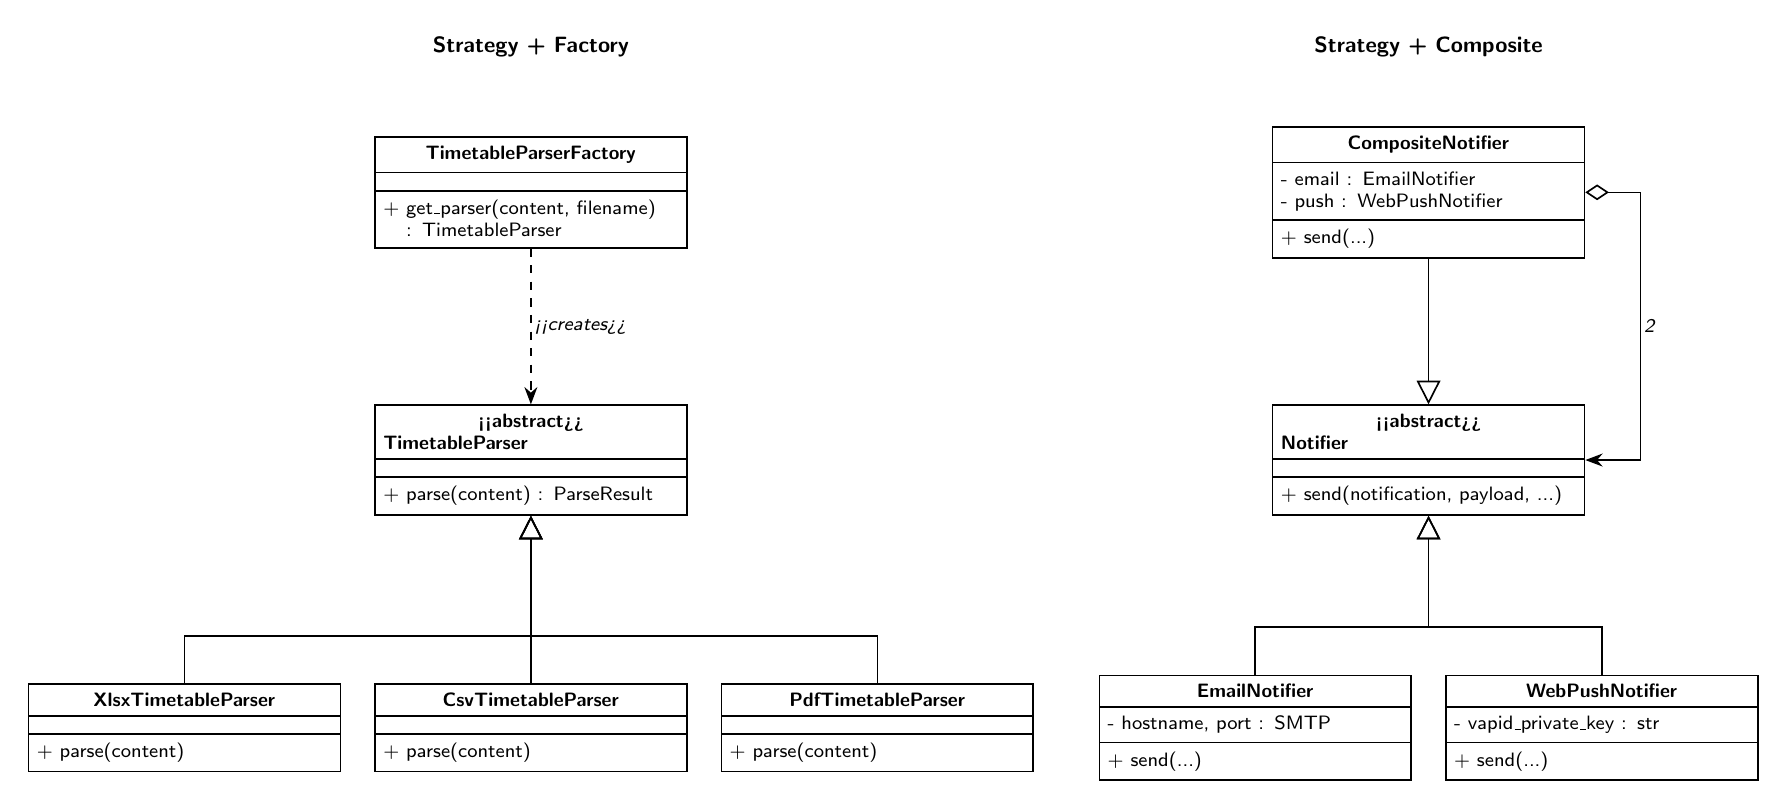
\begin{tikzpicture}[
    inh/.style={semithick, -{Triangle[open, length=3mm, width=3mm]}},
    dep/.style={semithick, dashed, -{Stealth[length=2.2mm]}},
    agg/.style={semithick, {Diamond[open, length=3mm, width=2mm]}-{Stealth[length=2.2mm]}},
    lbl/.style={font=\scriptsize\itshape, fill=white, inner sep=1pt}
  ]
  \umlclass{factory}{0,3.4}{TimetableParserFactory}{}{
    + get\_parser(content, filename)\\
    \phantom{+} : TimetableParser}
  \umlclass{parser}{0,0}{<{}<abstract>{}>\\TimetableParser}{}{
    + parse(content) : ParseResult}
  \umlclass{xlsx}{-4.4,-3.4}{XlsxTimetableParser}{}{+ parse(content)}
  \umlclass{csv}{0,-3.4}{CsvTimetableParser}{}{+ parse(content)}
  \umlclass{pdf}{4.4,-3.4}{PdfTimetableParser}{}{+ parse(content)}
  \draw[dep] (factory) -- node[lbl, right] {<{}<creates>{}>} (parser);
  \draw[inh] (xlsx.north) -- ++(0,0.6) -| (parser.south);
  \draw[inh] (csv.north) -- (parser.south);
  \draw[inh] (pdf.north) -- ++(0,0.6) -| (parser.south);
  \node[font=\footnotesize\bfseries, anchor=south] at (0,5.0) {Strategy + Factory};

  \umlclass{composite}{11.4,3.4}{CompositeNotifier}{
    - email : EmailNotifier\\
    - push : WebPushNotifier}{+ send(...)}
  \umlclass{notifier}{11.4,0}{<{}<abstract>{}>\\Notifier}{}{
    + send(notification, payload, ...)}
  \umlclass{email}{9.2,-3.4}{EmailNotifier}{
    - hostname, port : SMTP}{+ send(...)}
  \umlclass{push}{13.6,-3.4}{WebPushNotifier}{
    - vapid\_private\_key : str}{+ send(...)}
  \draw[inh] (composite.south) -- (notifier.north);
  \draw[agg] (composite.east) -- ++(0.7,0) |- node[lbl, pos=0.25, right] {2} (notifier.east);
  \draw[inh] (email.north) -- ++(0,0.6) -| (notifier.south);
  \draw[inh] (push.north) -- ++(0,0.6) -| (notifier.south);
  \node[font=\footnotesize\bfseries, anchor=south] at (11.4,5.0) {Strategy + Composite};
\end{tikzpicture}
}
  \caption{Class diagram of the Strategy, Factory and Composite patterns}
  \label{fig:classpatterns}
\end{figure}

\begin{figure}[!htbp]
  \centering
  \resizebox{\textwidth}{!}{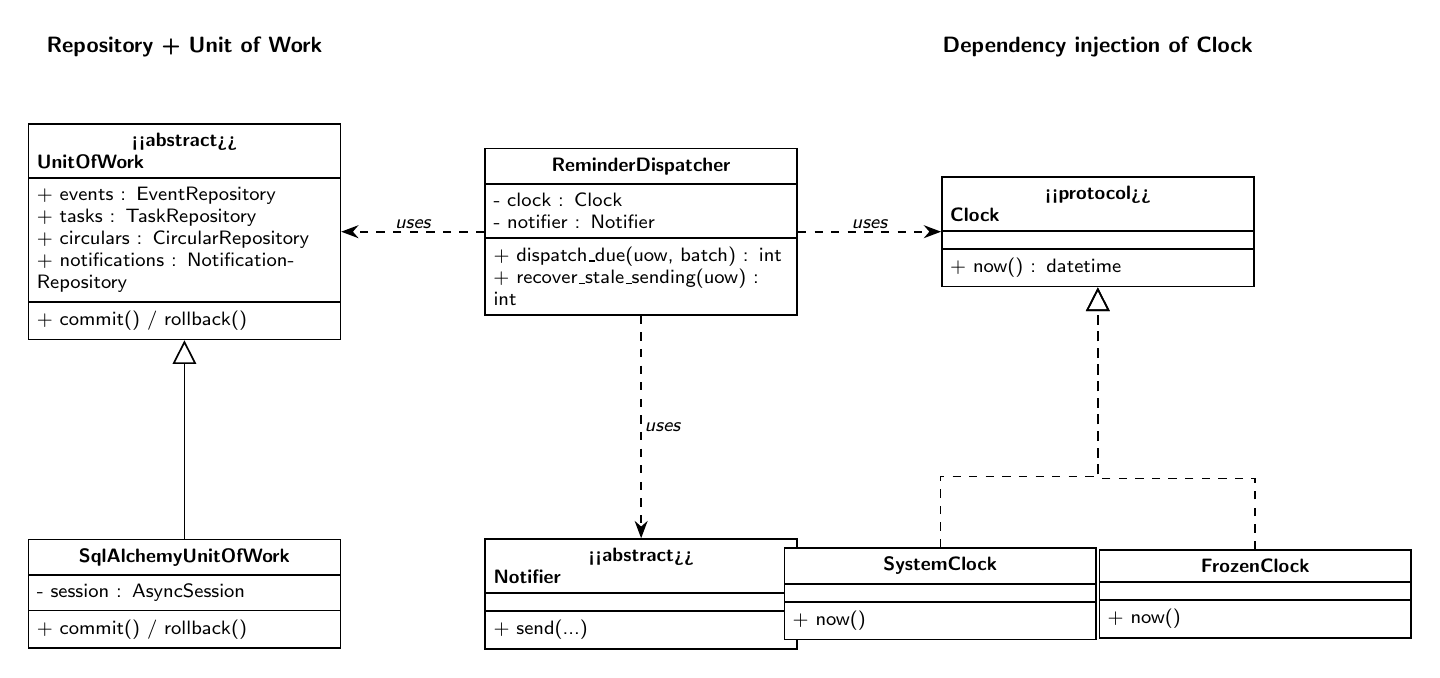
\begin{tikzpicture}[
    inh/.style={semithick, -{Triangle[open, length=3mm, width=3mm]}},
    real/.style={semithick, dashed, -{Triangle[open, length=3mm, width=3mm]}},
    dep/.style={semithick, dashed, -{Stealth[length=2.2mm]}},
    lbl/.style={font=\scriptsize\itshape, fill=white, inner sep=1pt}
  ]
  \umlclass{uow}{0,0}{<{}<abstract>{}>\\UnitOfWork}{
    + events : EventRepository\\
    + tasks : TaskRepository\\
    + circulars : CircularRepository\\
    + notifications : NotificationRepository}{
    + commit() / rollback()}
  \umlclass{sqlauow}{0,-4.6}{SqlAlchemyUnitOfWork}{
    - session : AsyncSession}{+ commit() / rollback()}
  \draw[inh] (sqlauow) -- (uow);
  \umlclass{disp}{5.8,0}{ReminderDispatcher}{
    - clock : Clock\\
    - notifier : Notifier}{
    + dispatch\_due(uow, batch) : int\\
    + recover\_stale\_sending(uow) : int}
  \umlclass{notif}{5.8,-4.6}{<{}<abstract>{}>\\Notifier}{}{+ send(...)}
  \umlclass{clock}{11.6,0}{<{}<protocol>{}>\\Clock}{}{+ now() : datetime}
  \umlclass{sysclock}{9.6,-4.6}{SystemClock}{}{+ now()}
  \umlclass{frozen}{13.6,-4.6}{FrozenClock}{}{+ now()}
  \draw[real] (sysclock.north) -- ++(0,0.9) -| (clock.south);
  \draw[real] (frozen.north) -- ++(0,0.9) -| (clock.south);
  \draw[dep] (disp) -- node[lbl, above] {uses} (uow);
  \draw[dep] (disp) -- node[lbl, above] {uses} (clock);
  \draw[dep] (disp) -- node[lbl, right] {uses} (notif);
  \node[font=\footnotesize\bfseries, anchor=south] at (0,2.1) {Repository + Unit of Work};
  \node[font=\footnotesize\bfseries, anchor=south] at (11.6,2.1) {Dependency injection of Clock};
\end{tikzpicture}
}
  \caption{Class diagram of the Repository and Unit of Work patterns and the injected Clock}
  \label{fig:classpatternsb}
\end{figure}

\subsection{Architecture Decisions}
\needspace{7\baselineskip}
\begin{xltabular}{\textwidth}{|p{3.4cm}|Y|}
\caption{Architecture decisions}\\
\hline
\textbf{Decision} & \textbf{Reason} \\ \hline
Background workers for slow work & OCR and timetable parsing take seconds; the API stores the file, replies \texttt{202 Accepted} and a Celery worker does the work, so every web request stays short. \\ \hline
UTC storage, local expansion & Every timestamp is stored in UTC. Weekly recurrence is expanded in local time (Asia/Kolkata) and then converted, so a 9:00 class stays at 9:00. \\ \hline
Injected clock & No code reads the system time directly; an injected \texttt{Clock} makes every time rule testable. \\ \hline
Exactly-once reminders & Key $k = \mathrm{SHA256}(\text{target}\,\|\,\text{user}\,\|\,\text{offset}\,\|\,\text{channel})$ with a unique database constraint; rows claimed with \texttt{FOR UPDATE SKIP LOCKED}. \\ \hline
Human in the loop & No OCR result reaches a calendar unless it passes the review gate and auto-confirmation is enabled; otherwise the HOD confirms it. \\ \hline
One authorisation policy & One \texttt{AuthorisationPolicy} class decides what Admin, HOD and Faculty may do, so permission rules live in one place. \\ \hline
\end{xltabular}

\newsection{Implementation (Algorithms Pseudo Code)}{sec:impl}

\subsection{Implementation Overview}
The backend has 76 Python source files and the frontend has eight main screens. Table~\ref{tab:files} maps each module to its main source files. The algorithms below are written from the code; each names the file it comes from. All times are in UTC unless marked local.

{\small
\needspace{7\baselineskip}
\begin{xltabular}{\textwidth}{|p{3.2cm}|Y|p{2.4cm}|}
\caption{Modules and source files}\label{tab:files}\\
\hline
\textbf{Module} & \textbf{Main source files (backend/app/)} & \textbf{Screen} \\ \hline
Identity and access & application/auth/*, application/security/policy.py, infrastructure/security/rate\_limiter.py & /login \\ \hline
Directory & application/directory/*, api/routers/directory.py & /directory \\ \hline
Timetable & application/timetable/*, infrastructure/parsers/* & /timetables \\ \hline
Circulars & application/circulars/use\_cases.py, infrastructure/ocr/* & /circulars \\ \hline
Calendar & application/calendar/* (clash\_detector, free\_slots, recurrence, ics\_service) & /calendar, /today \\ \hline
Reminders & application/reminders/* (planner, dispatcher, maths), infrastructure/notifiers/* & /settings \\ \hline
Tasks & application/tasks/*, workers/task\_alerts.py & /tasks \\ \hline
Operations & core/upload\_guard.py, infrastructure/storage/backup\_service.py & -- \\ \hline
\end{xltabular}}

\subsection{Algorithm 1: Three-Tier Initials Resolution}
A timetable cell such as \texttt{CN (KKS)} names the teacher by initials. The resolver tries an exact match, then an alias, and only then a fuzzy match based on the Levenshtein edit distance [7]. A fuzzy match is accepted only if it is clearly better than the second-best candidate, so the system never guesses between two similar teachers.
\begin{algorithm}[H]
\caption{Three-tier initials resolution (infrastructure/parsers/initials\_resolver.py)}
\begin{algorithmic}[1]
\Require token $t$, faculty profiles $F$; $\theta_{sim}=0.85$, $\theta_{margin}=0.10$
\State $t \gets \textsc{Upper}(\textsc{Trim}(t))$
\State $E \gets \{f \in F : f.\text{initials} = t\}$ \Comment{tier 1: exact initials}
\If{$|E| = 1$} \Return \textsc{Resolved}$(E_1)$ \ElsIf{$|E| > 1$} \Return \textsc{Ambiguous} \EndIf
\State $A \gets \{f \in F : t \in f.\text{aliases}\}$ \Comment{tier 2: exact alias}
\If{$|A| = 1$} \Return \textsc{Resolved}$(A_1)$ \ElsIf{$|A| > 1$} \Return \textsc{Ambiguous} \EndIf
\ForAll{$f \in F$} \Comment{tier 3: normalised similarity}
  \State $s_f \gets 1 - \textsc{Lev}(t, f.\text{initials}) / \max(|t|, |f.\text{initials}|)$
\EndFor
\State $s_1, s_2 \gets$ best and second-best scores
\If{$s_1 \ge \theta_{sim}$ \textbf{and} $s_1 - s_2 \ge \theta_{margin}$} \Return \textsc{Resolved}$(F_1)$ \EndIf
\State \Return \textsc{Unresolved} \Comment{shown to the HOD}
\end{algorithmic}
\end{algorithm}

\subsection{Algorithm 2: Sweep-Line Clash Detection}
Two events clash if their half-open intervals overlap: $\max(s_1, s_2) < \min(e_1, e_2)$. Events that only touch (one ends at 10:00, the next starts at 10:00) do not clash. Sorting by start time and keeping the currently open events in a min-heap finds all clashes in $O(n \log n + k)$ time for $k$ clashing pairs, instead of comparing every pair in $O(n^2)$.
\begin{algorithm}[H]
\caption{Sweep-line clash detection (application/calendar/clash\_detector.py)}
\begin{algorithmic}[1]
\Require intervals $I = \{[s_i, e_i)\}$
\State sort $I$ by $(s, e)$; $H \gets$ empty min-heap keyed by end time; $C \gets \emptyset$
\ForAll{$x \in I$ in sorted order}
  \While{$H \ne \emptyset$ \textbf{and} $\textsc{Min}(H).e \le x.s$} \State \textsc{Pop}$(H)$ \EndWhile
  \ForAll{$y \in H$} \State $C \gets C \cup \{(y, x)\}$ \EndFor
  \State \textsc{Push}$(H, x)$
\EndFor
\State \Return $C$
\end{algorithmic}
\end{algorithm}

\subsection{Algorithm 3: Weekly Class Generation}
Each confirmed timetable slot is expanded week by week inside the term and the current 21-day window. Holidays are skipped, and times are built in the term's local time zone before conversion to UTC.
\begin{algorithm}[H]
\caption{Class generation for one slot (application/calendar/recurrence.py)}
\begin{algorithmic}[1]
\Require slot (weekday, start, end), term $[d_0, d_1]$, holidays $D_h$, window $[w_0, w_1]$
\State $a \gets \max(d_0, w_0)$; $b \gets \min(d_1, w_1)$; \textbf{if} $a > b$ \textbf{return} $\emptyset$
\ForAll{date $d \in \textsc{WeeklyRule}(a, b, \text{weekday})$}
  \If{$d \notin D_h$}
    \State $s \gets \textsc{ToUTC}(d + \text{start})$; $e \gets \textsc{ToUTC}(d + \text{end})$ \Comment{local $\rightarrow$ UTC}
    \State emit occurrence $(d, s, e)$
  \EndIf
\EndFor
\end{algorithmic}
\end{algorithm}

\subsection{Algorithm 4: Reminder Planning with Quiet Hours}
For each attendee, lead time and channel, the fire time is the event start minus the lead time. If that falls inside the user's quiet window, the reminder moves to the end of the window, unless the event starts before the window ends (an early-morning class), in which case it is kept. A SHA-256 key makes planning repeatable without duplicates.
\begin{algorithm}[H]
\caption{Reminder planning (application/reminders/planner.py, maths.py)}
\begin{algorithmic}[1]
\Require event $E$; per-user rule (offsets $O$, channels $K$) or the default for $E.\text{kind}$
\ForAll{attendee user $u$, offset $o \in O$, channel $c \in K$}
  \State $f \gets E.s - o$
  \If{local time of $f$ lies in $u$'s quiet window $[q_s, q_e)$}
    \State $w \gets$ end of that window in UTC (next day if the window crosses midnight)
    \If{$E.s > w$} $f \gets w$ \EndIf
  \EndIf
  \State $k \gets \mathrm{SHA256}(E.\text{id} \,\|\, u \,\|\, o \,\|\, c)$
  \If{no notification with key $k$ exists} save a PENDING notification $(u, c, f, k)$ \EndIf
\EndFor
\end{algorithmic}
\end{algorithm}

\subsection{Algorithm 5: Reminder Dispatch}
Every 30 seconds the dispatcher claims a batch of due reminders under a row lock that other workers skip, and sends each one. Failed sends are designed to be retried after a random delay up to $\min(1800, 30 \cdot 2^{n})$ seconds (full-jitter back-off).
\begin{algorithm}[H]
\caption{Reminder dispatch (application/reminders/dispatcher.py)}
\begin{algorithmic}[1]
\State \textbf{transaction:} claim up to 100 rows with status PENDING and fire time $\le$ now \texttt{FOR UPDATE SKIP LOCKED}; mark them SENDING; attempts $+{=}\,1$
\ForAll{claimed notification $n$}
  \If{target task is already done} \textsc{Cancel}$(n)$; \textbf{continue} \EndIf
  \If{\textsc{Send}$(n)$ succeeds} \textsc{MarkSent}$(n)$
  \Else
    \State $\delta \gets \textsc{Uniform}(0, \min(1800, 30 \cdot 2^{\text{attempts}}))$
    \If{attempts $< 5$} reschedule $n$ at now $+ \delta$ \Else\ \textsc{MarkFailed}$(n)$ \EndIf
  \EndIf
\EndFor
\end{algorithmic}
\end{algorithm}

\subsection{Algorithm 6: Task Priority Score}
Each active task gets a score between 0 and 1 that balances importance and urgency; urgency decays exponentially with the hours left, with a time constant of 48 hours. Overdue tasks score between 1 and 2, so they always rank first, and completed tasks score $-1$.
\begin{algorithm}[H]
\caption{Task priority score (application/tasks/maths.py)}
\begin{algorithmic}[1]
\Require importance $I \in \{1..5\}$, deadline $D$, now $T$; $w_I = 0.4$, $w_U = 0.6$, $\tau = 48$ h
\If{task is completed} \Return $-1$ \EndIf
\State $h \gets (D - T)$ in hours
\If{$h \le 0$} \Return $1 + \min(|h|/24, 7)/7$ \EndIf
\State \Return $w_I \cdot (I-1)/4 + w_U \cdot e^{-h/\tau}$
\end{algorithmic}
\end{algorithm}

\subsection{Algorithm 7: Circular Review Gate}
The OCR confidence of a document is the length-weighted mean of its word confidences, $C = \sum \ell_i c_i / \sum \ell_i$, so long words count more than short ones. A circular is confirmed automatically only if every condition below holds.
\begin{algorithm}[H]
\caption{Circular review gate (infrastructure/ocr/extractor.py)}
\begin{algorithmic}[1]
\Require document confidence $C$, field confidences $C_{date}$, $C_{time}$, attendees $A$
\If{$C \ge 70$ \textbf{and} $C_{date} \ge 0.85$ \textbf{and} $C_{time} \ge 0.85$ \textbf{and} $|A| \ge 1$ \textbf{and} $\forall a \in A: C_a \ge 0.85$ \textbf{and not} duplicate}
  \If{department allows automatic confirmation} \Return CONFIRMED \EndIf
\EndIf
\State \Return NEEDS\_REVIEW (with the list of reasons)
\end{algorithmic}
\end{algorithm}

\newsection{Results}{sec:results}

All results in this section were produced on 13 November 2026 on a laptop (Apple Silicon, macOS, Python 3.12.14) against the running Docker Compose stack. The raw outputs are saved in the project under \texttt{report/latex/results/}.

\subsection{Automated Backend Tests}
The backend test suite was run with \texttt{pytest}: \textbf{83 tests passed and 0 failed} in 11.1 seconds. Of these, 68 are unit tests of the business rules and algorithms, and 15 are integration tests that run against real PostgreSQL 16 and Redis 7.

\needspace{7\baselineskip}
\begin{xltabular}{\textwidth}{|p{5.2cm}|>{\centering\arraybackslash}p{1.3cm}|Y|}
\caption{Backend test results by file}\\
\hline
\textbf{Test file} & \textbf{Tests} & \textbf{What it checks} \\ \hline
unit/test\_domain\_invariants & 10 & Entity validation and state-machine transitions \\ \hline
unit/test\_hardening & 10 & File-type sniffing, size, pixel and page limits \\ \hline
unit/test\_task\_maths & 9 & Priority score ranges, alert times, completion rate \\ \hline
unit/test\_ocr\_maths & 8 & Length-weighted confidence, time grammar, deskew \\ \hline
unit/test\_parsers & 6 & Excel merged cells, CSV, PDF tables, cell tokens \\ \hline
unit/test\_initials\_matching & 4 & Exact, alias, fuzzy and ambiguous initials \\ \hline
unit/test\_reminder\_maths & 4 & Fire time, idempotency key, back-off, quiet hours \\ \hline
7 other unit files & 17 & Clash detection, free slots, recurrence, ICS, clock, policy, bulk import \\ \hline
8 integration files & 15 & Log-in flow, timetable, circular, calendar, task and reminder pipelines, rate limiter, repositories \\ \hline
\textbf{Total} & \textbf{83} & \textbf{All passed} \\ \hline
\end{xltabular}

\subsection{End-to-End Browser Tests}
Four user journeys were run in a real Chromium browser with Playwright against the running frontend and API: \textbf{4 passed} in 12.9 seconds.

\needspace{7\baselineskip}
\begin{xltabular}{\textwidth}{|>{\centering\arraybackslash}p{1.2cm}|Y|>{\centering\arraybackslash}p{1.4cm}|>{\centering\arraybackslash}p{1.4cm}|}
\caption{End-to-end test results}\\
\hline
\textbf{No.} & \textbf{Journey verified in the browser} & \textbf{Result} & \textbf{Time} \\ \hline
1 & HOD uploads \texttt{standard\_timetable.xlsx} and confirms; faculty KKS sees the classes on the calendar & Pass & 3.7 s \\ \hline
2 & Faculty uploads a circular; HOD reviews and confirms; attendees see the meeting & Pass & 5.0 s \\ \hline
3 & A scheduled meeting produces a notification record marked SENT & Pass & 0.6 s \\ \hline
4 & HOD assigns a template task; faculty completes it; pending alerts are resolved & Pass & 2.2 s \\ \hline
\end{xltabular}

\subsection{Algorithm Outputs on Worked Examples}
The values below were computed by calling the project's own functions with the time fixed at 04:30 UTC on 13 November 2026 (script \texttt{results/worked\_examples.py}).

\head{Task Priority Score}
\begin{table}[H]
\centering
\begin{tabular}{|p{4.8cm}|>{\centering\arraybackslash}p{2.2cm}|>{\centering\arraybackslash}p{3.2cm}|>{\centering\arraybackslash}p{2.4cm}|}
\hline
\textbf{Task} & \textbf{Importance} & \textbf{Hours to deadline} & \textbf{Priority $P$} \\ \hline
IA marks upload & 5 & 6 & 0.9295 \\ \hline
CO--PO mapping & 4 & 48 & 0.5207 \\ \hline
Lab manual update & 2 & 240 & 0.1040 \\ \hline
Course file submission & 3 & $-36$ (overdue) & 1.2143 \\ \hline
\end{tabular}
\caption{Priority scores of four sample tasks}
\end{table}
The overdue task ranks first, then the urgent high-importance task. For example, IA marks upload scores $0.4 \times 4/4 + 0.6 \times e^{-6/48} = 0.4 + 0.5295 = 0.9295$.

\head{Initials Similarity}
\begin{table}[H]
\centering
\begin{tabular}{|p{2.6cm}|p{2.6cm}|>{\centering\arraybackslash}p{2.4cm}|p{5.2cm}|}
\hline
\textbf{Token} & \textbf{Candidate} & \textbf{Similarity} & \textbf{Decision} \\ \hline
KKS & KKS & 1.000 & Match (exact) \\ \hline
PARKAVI & PARKAVY & 0.857 & Fuzzy match if margin $\ge 0.10$ \\ \hline
KKS & KSS & 0.667 & Rejected (below 0.85) \\ \hline
RNS & KKS & 0.333 & Rejected \\ \hline
\end{tabular}
\caption{Normalised Levenshtein similarity examples}
\end{table}

\head{Other Worked Examples}
\begin{itemize}
  \item \textbf{Quiet hours:} a 10:00 IST class on 14 November with a 12-hour reminder would fire at 22:00 IST, inside a 22:00--07:00 quiet window. The planner moved it to 07:00 IST (01:30 UTC), still before the class.
  \item \textbf{Task alerts:} a task due in 5 days produced alerts exactly 72 hours, 24 hours and 2 hours before the deadline.
  \item \textbf{OCR confidence:} the words ``Meeting on 18/11/2026 at 2:30 PM'' with confidences 96, 91, 72, 88, 65 and 90 give a length-weighted confidence of $2190/27 = 81.11$, above the gate of 70.
\end{itemize}

\subsection{Clash Detection Performance}
Random 50, 60 or 120-minute events were placed on a 15-minute grid over 30 days (fixed random seed 20261113). The sweep-line detector and the brute-force pairwise check returned identical clash sets at every size.

\begin{table}[H]
\centering
\begin{tabular}{|>{\centering\arraybackslash}p{2.2cm}|>{\centering\arraybackslash}p{2.4cm}|>{\centering\arraybackslash}p{2.6cm}|>{\centering\arraybackslash}p{2.6cm}|>{\centering\arraybackslash}p{2.2cm}|}
\hline
\textbf{Events $n$} & \textbf{Clash pairs} & \textbf{Sweep line (ms)} & \textbf{Pairwise (ms)} & \textbf{Same result} \\ \hline
500 & 444 & 0.14 & 4.53 & Yes \\ \hline
1,000 & 1,667 & 0.31 & 25.78 & Yes \\ \hline
2,000 & 6,697 & 0.91 & 74.34 & Yes \\ \hline
4,000 & 26,822 & 2.47 & 299.06 & Yes \\ \hline
\end{tabular}
\caption{Sweep-line versus brute-force clash detection (one run per size)}
\end{table}

\begin{figure}[!htbp]
\centering
\begin{tikzpicture}
  \begin{scope}[x=0.0028cm, y=0.022cm]
    \draw[semithick, -{Stealth[length=2mm]}] (0,0) -- (4300,0) node[below left, font=\scriptsize] {events $n$};
    \draw[semithick, -{Stealth[length=2mm]}] (0,0) -- (0,330) node[above, font=\scriptsize] {time (ms)};
    \foreach \x in {1000,2000,3000,4000} \draw (\x,0) -- (\x,-5) node[below, font=\tiny] {\x};
    \foreach \y in {100,200,300} \draw (0,\y) -- (-60,\y) node[left, font=\tiny] {\y};
    \draw[semithick] (500,4.53) -- (1000,25.78) -- (2000,74.34) -- (4000,299.06);
    \foreach \p in {(500,4.53),(1000,25.78),(2000,74.34),(4000,299.06)} \fill \p circle (1.4pt);
    \draw[semithick, dashed] (500,0.14) -- (1000,0.31) -- (2000,0.91) -- (4000,2.47);
    \foreach \p in {(500,0.14),(1000,0.31),(2000,0.91),(4000,2.47)} \draw[fill=white] \p circle (1.4pt);
    \node[font=\scriptsize, anchor=west] at (3000,240) {pairwise $O(n^2)$};
    \node[font=\scriptsize, anchor=west] at (3000,25) {sweep line $O(n \log n + k)$};
  \end{scope}
\end{tikzpicture}
\caption{Clash detection time against the number of events}
\end{figure}

\subsection{Database Benchmark (Recorded Earlier)}
During the hardening stage on 28 October 2026, a benchmark script loaded 120 faculty, 5,000 tasks and two terms. A one-week calendar query took 0.60 ms at the 95th percentile, and claiming 1,000 due notifications took 1.2 ms. This benchmark was not rerun for this report.

\subsection{Application Screens}
The screens below were captured by an automated Playwright script from the running application, logged in with the seeded test accounts.

\begin{figure}[!htbp]
  \centering
  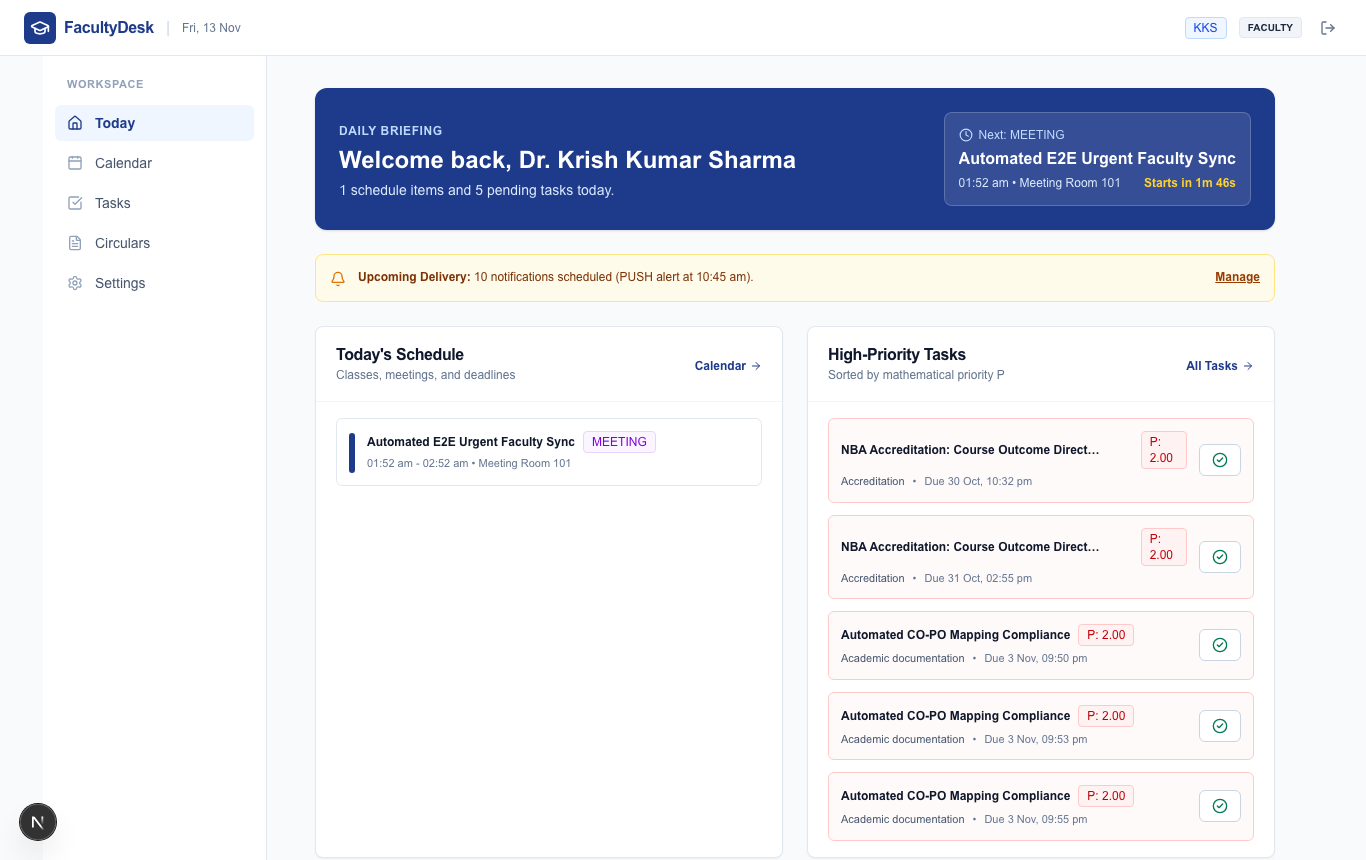
\includegraphics[width=0.92\textwidth]{figures/screens/faculty-today.png}
  \caption{Faculty ``Today'' screen: next meeting countdown, today's schedule and high-priority tasks}
\end{figure}
\begin{figure}[!htbp]
  \centering
  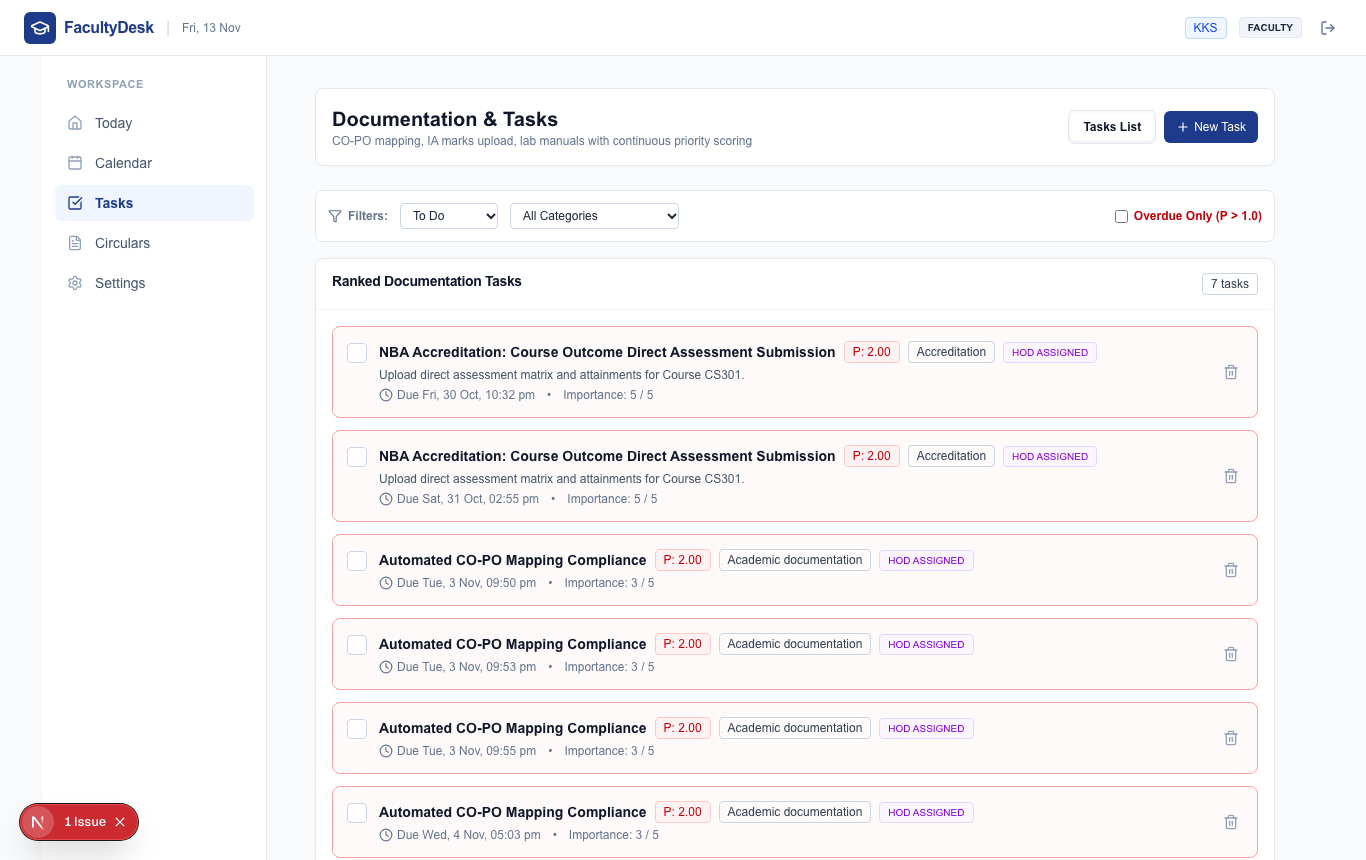
\includegraphics[width=0.92\textwidth]{figures/screens/faculty-tasks.png}
  \caption{Documentation tasks ranked by priority score $P$ (overdue tasks have $P > 1$)}
\end{figure}
\begin{figure}[!htbp]
  \centering
  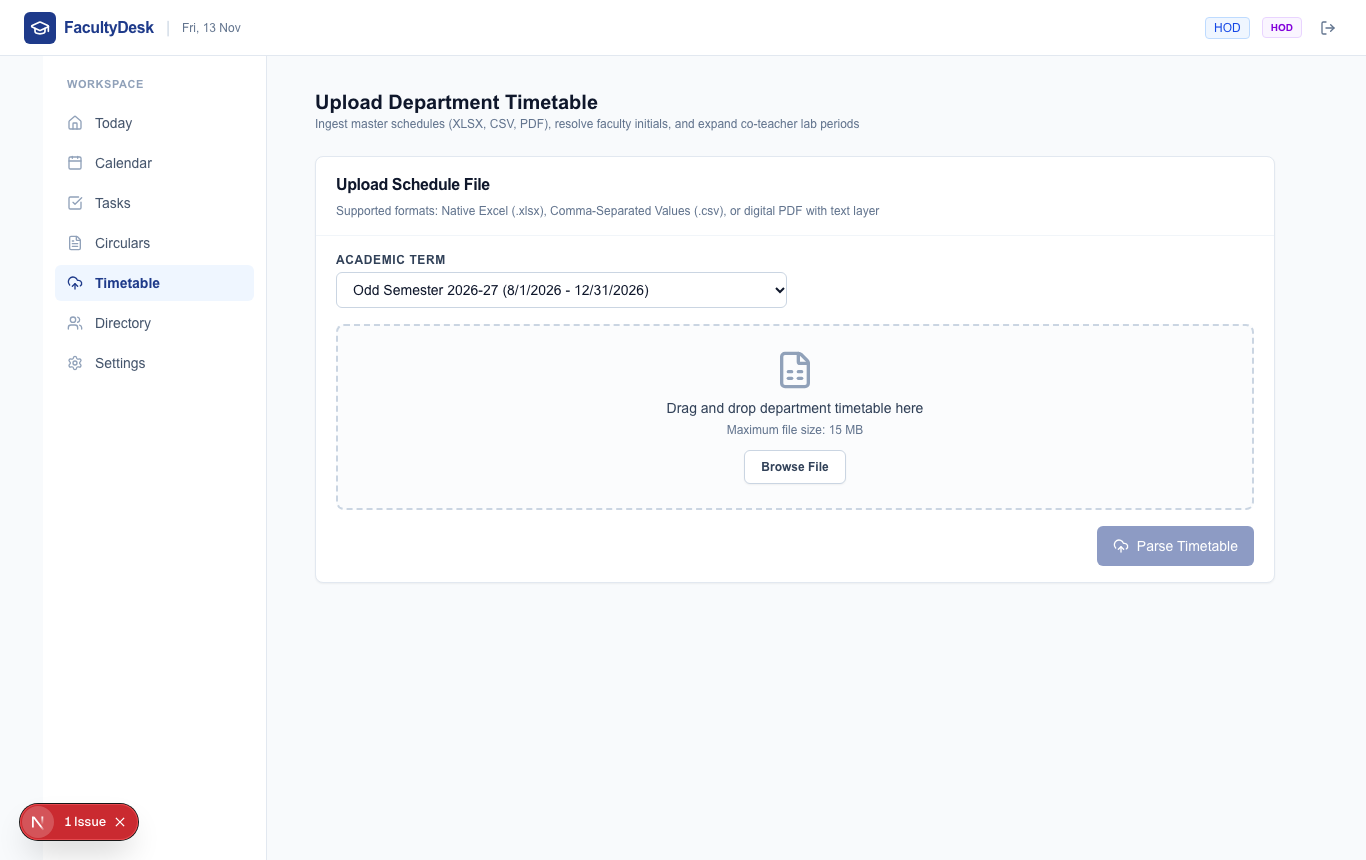
\includegraphics[width=0.92\textwidth]{figures/screens/hod-timetables.png}
  \caption{HOD timetable upload screen}
\end{figure}
\begin{figure}[!htbp]
  \centering
  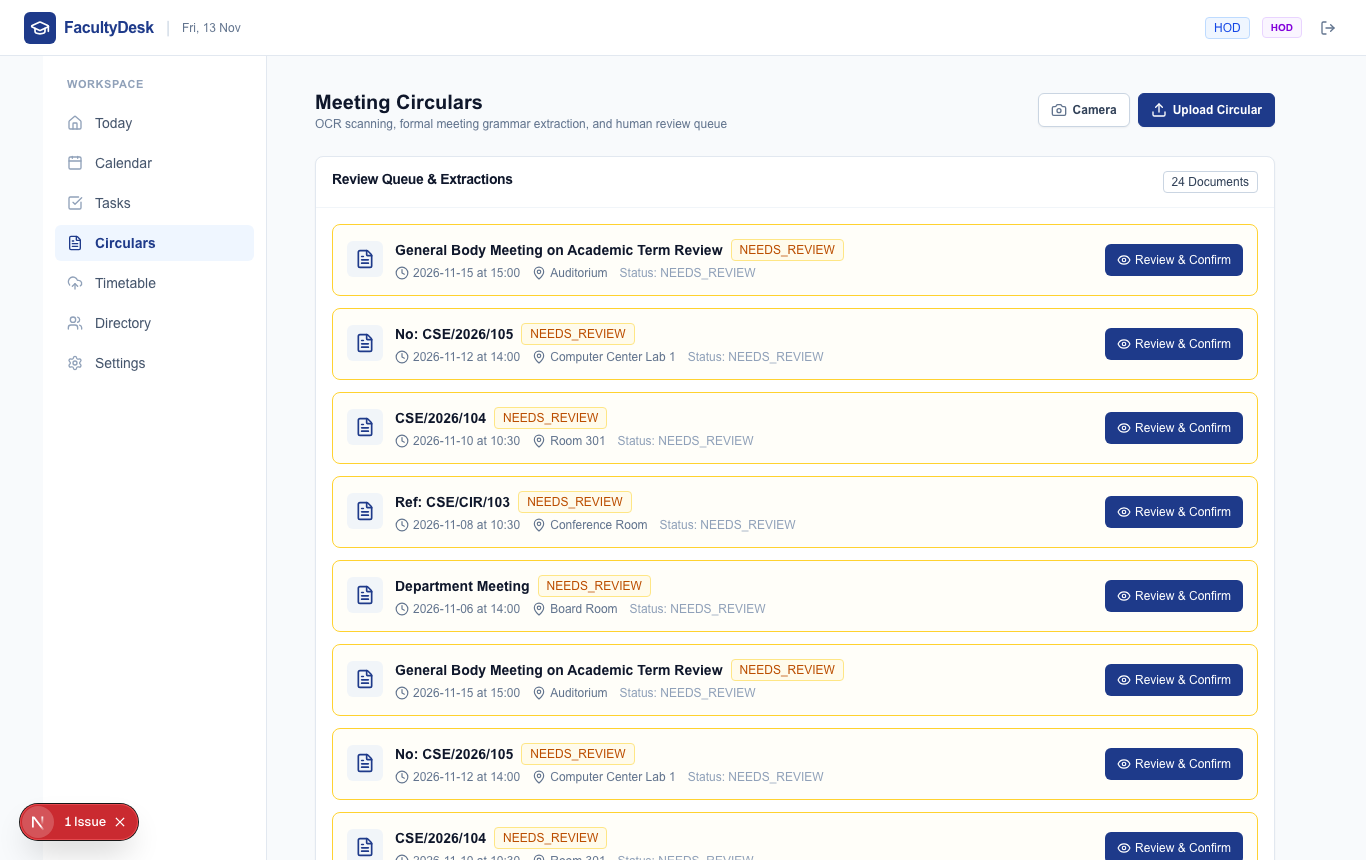
\includegraphics[width=0.92\textwidth]{figures/screens/hod-circulars.png}
  \caption{HOD circular review queue with OCR-extracted date, time and venue}
\end{figure}
\begin{figure}[!htbp]
  \centering
  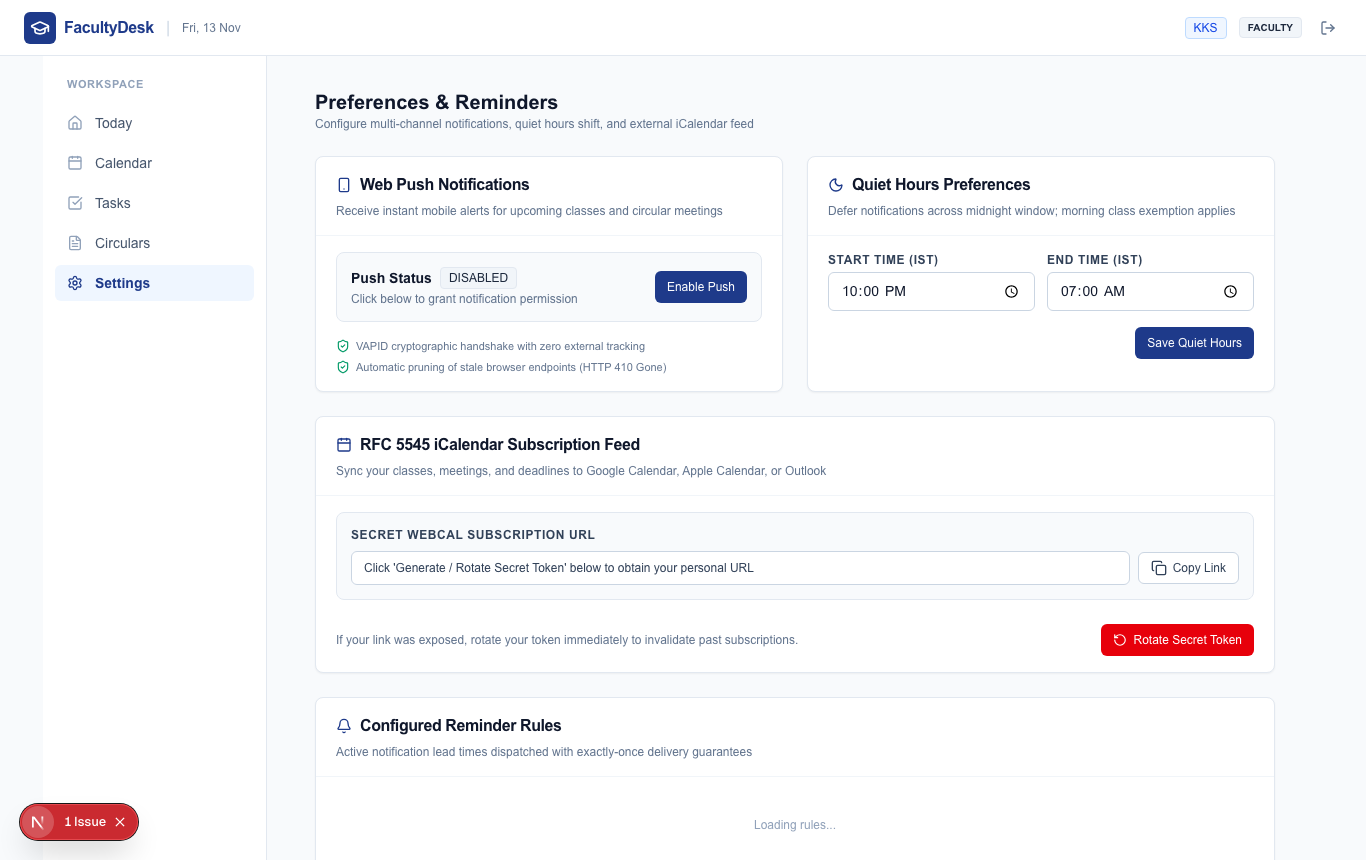
\includegraphics[width=0.92\textwidth]{figures/screens/faculty-settings.png}
  \caption{Reminder settings: web push, quiet hours and private ICS feed}
\end{figure}

\newsection{Discussion of Results}{sec:discussion}

\subsection{What the Results Show}
The 83 backend tests and the 4 browser journeys confirm that the main business flows work end to end on the running system: a timetable becomes classes on a teacher's calendar, a circular becomes a confirmed meeting, a reminder is recorded as sent, and an assigned task can be completed with its alerts resolved. The object-oriented design is what made this testable: because the domain classes contain no framework code, 68 unit tests check the business rules in 3.3 seconds without a database.

\subsection{Clash Detection}
The sweep-line detector agreed with the brute-force check on every random instance, and its advantage grew with size: 32 times faster at 500 events and 121 times faster at 4,000 events. This matches the expected $O(n \log n + k)$ against $O(n^2)$ behaviour. One faculty member has only a few hundred events per term, so both methods are fast enough for a single person; the gain matters when the clash check and free-slot finder run across a whole department. The timings come from one run per size on one laptop and should be read as indicative.

\subsection{Initials Matching}
The worked examples show a deliberate trade-off. Two three-letter initials that differ by one letter have a similarity of 0.667, below the threshold of 0.85, so fuzzy matching helps only with longer tokens such as names or aliases with a typo. For short initials the system relies on exact and alias matches and reports anything else to the HOD. A missed match can be fixed by adding an alias; a wrong match would put classes on the wrong teacher's calendar, so the design prefers the first.

\subsection{Limitations Found During Testing}
\needspace{7\baselineskip}
\begin{xltabular}{\textwidth}{|p{3.4cm}|Y|Y|}
\caption{Limitations and planned fixes}\\
\hline
\textbf{Limitation} & \textbf{Observation} & \textbf{Planned fix} \\ \hline
Reminder retry path & When a send fails, the dispatcher calls \texttt{retry()} while the reminder is still SENDING, which the state table does not allow. The failed reminder and the rest of its batch wait for stale recovery (5 minutes) instead of the designed back-off. Reminders are still sent at most once. & Move the reminder to FAILED before \texttt{retry()}; add a test with a notifier that fails. \\ \hline
Re-confirming a timetable & Confirming the same timetable again creates duplicate class events, because earlier generated events are not replaced. & On confirmation, replace the previous upload's future class events, keyed by slot and date. \\ \hline
Layering & Four application files import infrastructure classes directly. & Move OCR, parser and storage behind domain interfaces. \\ \hline
No field pilot & OCR accuracy on real department circulars, time saved and user satisfaction were not measured. & Run a one-semester pilot in one department. \\ \hline
Scanned timetables & Timetable PDFs without a text layer are rejected rather than read with OCR. & Add OCR for scanned timetable PDFs. \\ \hline
\end{xltabular}

\subsection{Comparison with the 2026 Literature}
The timetabling papers surveyed in Section~\ref{sec:literature} focus on \emph{generating} timetables by optimisation or rules. FacultyDesk takes the timetable as given and focuses on \emph{distributing} it to individuals, combining it with meetings and tasks, and reminding people. The document-AI papers report that modern vision--language models can extract fields from scanned documents and that a multi-stage pipeline with preprocessing improves accuracy. FacultyDesk follows the multi-stage approach with classical Tesseract OCR, which runs on a department server without a GPU; replacing the extractor with a small vision--language model is a possible extension at a higher hardware cost.

\newsection{Conclusion}{sec:conclusion}

FacultyDesk shows that a department's existing documents, a timetable spreadsheet and photos of paper circulars, can be turned into a personal, clash-aware calendar with reminders for every faculty member, without anyone retyping information. The system covers eight modules: identity and access, directory and academic calendar, timetable ingestion, circular scanning, calendar, reminders, tasks with escalation, and operations.

Object-oriented analysis and design shaped the whole project. Noun analysis of the problem statement produced twenty domain classes that hold their own rules, three of which enforce their life cycles as state machines. The UML models (use case, class, sequence, collaboration, statechart, activity, package, component and deployment diagrams) describe the system from the user's view down to the deployed containers, and every name in them matches the code. A four-layer architecture kept the business rules free of web, database and queue code, and the Repository, Unit of Work, Strategy, Factory, Composite and State patterns each solved a concrete problem: storage independence, atomic multi-object updates, new file formats and channels without changing existing code, and safe status changes.

On 13 November 2026 all 83 backend tests and all 4 end-to-end journeys passed on the running system, and the sweep-line clash detector matched brute force exactly while running up to 121 times faster on 4,000 events.

\subsection{Future Work}
\begin{itemize}
  \item Fix the reminder retry path and the duplicate classes on re-confirmation, with regression tests.
  \item Run a pilot in one department to measure OCR accuracy on real circulars, reminder delivery and time saved for the HOD.
  \item Read scanned timetable PDFs with OCR, and evaluate a small vision--language model for circular extraction.
  \item Complete the layering by moving OCR, parsing and storage behind domain interfaces.
  \item Add SMS or WhatsApp as a further notification channel through a new \texttt{Notifier} strategy.
\end{itemize}

\newsection{References}{sec:references}

\begin{enumerate}[label={[\arabic*]}, leftmargin=*, itemsep=6pt]
  \item Grady Booch, James Rumbaugh, Ivar Jacobson, \textit{The Unified Modeling Language User Guide}, 2nd Edition, Addison-Wesley, 2005.
  \item Craig Larman, \textit{Applying UML and Patterns: An Introduction to Object-Oriented Analysis and Design and Iterative Development}, 3rd Edition, Prentice Hall, 2004.
  \item Erich Gamma, Richard Helm, Ralph Johnson, John Vlissides, \textit{Design Patterns: Elements of Reusable Object-Oriented Software}, Addison-Wesley, 1994.
  \item Martin Fowler, \textit{Patterns of Enterprise Application Architecture}, Addison-Wesley, 2002.
  \item Robert C. Martin, \textit{Clean Architecture: A Craftsman's Guide to Software Structure and Design}, Prentice Hall, 2017.
  \item Ray Smith, ``An Overview of the Tesseract OCR Engine,'' \textit{Proc. 9th International Conference on Document Analysis and Recognition (ICDAR)}, 2007, pp. 629--633.
  \item V. I. Levenshtein, ``Binary codes capable of correcting deletions, insertions, and reversals,'' \textit{Soviet Physics Doklady}, vol. 10, no. 8, pp. 707--710, 1966.
  \item B. Desruisseaux (Ed.), ``Internet Calendaring and Scheduling Core Object Specification (iCalendar),'' IETF RFC 5545, 2009.
  \item J. Shen, P. Yuan, A. Ghosh, Y. Mai, D. Dahlmeier, ``OCR or Not? Rethinking Document Information Extraction in the MLLMs Era with Real-World Large-Scale Datasets,'' arXiv:2603.02789, March 2026.
  \item Y. Han, Y. Zhang, Y. Wang, Y. Jin, K. Z. Ke, J. Zhao, ``A Multistage Extraction Pipeline for Long Scanned Financial Documents: An Empirical Study in Industrial KYC Workflows,'' arXiv:2604.26462, April 2026.
  \item Y. Fehlis \textit{et al.}, ``Operationalizing Document AI: A Microservice Architecture for OCR and LLM Pipelines in Production,'' arXiv:2605.18818, May 2026.
  \item M. Elhüseyni, ``Course Timetabling under Conflict and Lecturer Preferences using Bi-objective Optimization Model,'' arXiv:2607.03901, July 2026.
  \item H. Sharafuddin, ``Automated University Timetabling: An AI Approach for Efficient Schedule Management,'' \textit{International Journal of Emerging Technologies in Learning (iJET)}, vol. 21, no. 2, pp. 91--99, 2026, doi: 10.3991/ijet.v21i02.59329.
\end{enumerate}

\newsection{Literature Survey Proofs}{sec:literature}

Five papers published in 2026 that relate to FacultyDesk were surveyed: two on university timetabling and three on extracting information from scanned documents. Each entry below was checked on the paper's official page (the journal page or the arXiv page) on 13 November 2026. The title, authors, date and identifier are copied from that page, and a screenshot of the page is included as proof. The summaries are our own, written from the abstracts.

\newcommand{\paperentry}[7]{%
\needspace{7\baselineskip}
\subsection{#1}
\begin{xltabular}{\textwidth}{|p{3.2cm}|Y|}
\hline
\textbf{Authors} & #2 \\ \hline
\textbf{Published} & #3 \\ \hline
\textbf{Identifier} & #4 \\ \hline
\textbf{Summary} & #5 \\ \hline
\textbf{Relevance to FacultyDesk} & #6 \\ \hline
\end{xltabular}
\begin{figure}[H]
\centering
\fbox{\includegraphics[width=0.92\textwidth, trim=0 330 0 0, clip]{figures/papers/#7.png}}
\caption{Proof: official page of ``#1''}
\end{figure}}

\paperentry{Automated University Timetabling: An AI Approach for Efficient Schedule Management}
{Hassan Sharafuddin (Arab Open University, Kuwait)}
{29 April 2026, \textit{International Journal of Emerging Technologies in Learning (iJET)}, vol. 21, no. 2, pp. 91--99}
{DOI: \href{https://doi.org/10.3991/ijet.v21i02.59329}{10.3991/ijet.v21i02.59329}}
{Describes Arab Open University's move from manual timetabling to a rule-based Python scheduling system serving about 62,000 students and over 1,000 staff across nine branches. The author reports timetable creation falling from four to six weeks to under two hours, 85\% fewer conflicts, and room utilisation rising from 65\% to 78\%, and argues that transparent rules suit institutions better than black-box optimisers.}
{Supports our choice of transparent, explainable rules (initials tiers, review gate, priority formula). The paper builds timetables; FacultyDesk distributes them to each teacher.}
{paper-ijet-59329}

\paperentry{Course Timetabling under Conflict and Lecturer Preferences using Bi-objective Optimization Model}
{Murat Elhüseyni}
{Submitted 4 July 2026, arXiv (Optimization and Control)}
{arXiv: \href{https://arxiv.org/abs/2607.03901}{2607.03901}}
{Formulates a real course timetabling problem with lecturer rest periods and theory-before-practical precedence as a bi-objective mixed-integer linear program. On a real dataset it reduces course conflicts by 13.33\% and improves lecturer schedule compactness by 26\% compared with the actual timetable.}
{Its notion of a conflict matches our half-open interval test for clash detection. It generates timetables, whereas FacultyDesk reads and distributes them.}
{paper-arxiv-2607.03901}

\paperentry{OCR or Not? Rethinking Document Information Extraction in the MLLMs Era with Real-World Large-Scale Datasets}
{Jiyuan Shen, Peiyue Yuan, Atin Ghosh, Yifan Mai, Daniel Dahlmeier}
{Submitted 3 March 2026, arXiv (Computation and Language)}
{arXiv: \href{https://arxiv.org/abs/2603.02789}{2603.02789}}
{Benchmarks multimodal large language models on business-document information extraction and finds that image-only input can perform comparably to pipelines that add OCR text, with careful schemas and instructions improving results.}
{A possible future replacement for our Tesseract-plus-rules extractor, at the cost of GPU hardware.}
{paper-arxiv-2603.02789}

\paperentry{A Multistage Extraction Pipeline for Long Scanned Financial Documents: An Empirical Study in Industrial KYC Workflows}
{Yuxuan Han, Yuanxing Zhang, Yushuo Wang, Yichao Jin, Kenneth Zhu Ke, Jingyuan Zhao}
{Submitted 29 April 2026, arXiv (Computer Vision)}
{arXiv: \href{https://arxiv.org/abs/2604.26462}{2604.26462}}
{Proposes a multistage pipeline (image preprocessing, multilingual OCR, page retrieval and compact vision--language extraction) for long scanned KYC documents. On 120 production documents (about 3,000 pages) it beats direct PDF-to-model baselines by up to 31.9 percentage points; the best setup reaches 87.27\% field accuracy.}
{Supports our design of preprocessing images before OCR and separating text extraction from field extraction.}
{paper-arxiv-2604.26462}

\paperentry{Operationalizing Document AI: A Microservice Architecture for OCR and LLM Pipelines in Production}
{Yao Fehlis, Benjamin Bengfort, Zhangzhang Si, Vahid Eyorokon, Prema Roman, Patrick Deziel, Devon Slonaker, Steve Veldman, Ben Johnson, Joyce Rigelo, Michael Wharton, Steve Kramer}
{Submitted 12 May 2026, arXiv (Artificial Intelligence)}
{arXiv: \href{https://arxiv.org/abs/2605.18818}{2605.18818}}
{Presents a microservice architecture for production document AI with classification, OCR and language-model field extraction, separating CPU orchestration from GPU inference and using asynchronous I/O. Profiling shows that OCR, not language-model parsing, dominates end-to-end latency.}
{Matches our decision to run OCR asynchronously in Celery workers so that web requests return immediately with \texttt{202 Accepted}.}
{paper-arxiv-2605.18818}

\subsection*{Gap Addressed by FacultyDesk}
The timetabling work optimises how a timetable is built, and the document-AI work improves how fields are read from scans. None of the surveyed papers addresses what happens after both: delivering one combined, clash-checked schedule to each faculty member with reliable reminders and documentation tracking. That is the part FacultyDesk covers.


\end{document}
